\documentclass[11pt]{report}

% ==================== Lingua e caratteri ====================
\usepackage[utf8]{inputenc}
\usepackage[T1]{fontenc}
\usepackage{lmodern}
\usepackage[italian]{babel}
\DeclareUnicodeCharacter{03BC}{\textmu}   % carattere μ (micro)
\DeclareUnicodeCharacter{00B5}{\textmu}   % carattere µ (micro)

% ==================== Titoli dei capitoli ====================
\usepackage{titlesec}
\titleformat{\chapter}
  {\normalfont\LARGE\bfseries}{\thechapter}{1em}{}
\titlespacing*{\chapter}{0pt}{3.5ex plus 1ex minus .2ex}{2.3ex plus .2ex}

% ==================== Impaginazione e pacchetti ====================
\usepackage{tabularx}
\usepackage[margin=1.2in]{geometry}
\usepackage[toc,page]{appendix}
\usepackage{graphicx}
\usepackage{caption}
\usepackage{subcaption}
\usepackage{float}
\usepackage{tikz}
\usepackage{forest}
\usetikzlibrary{trees, shapes.geometric, arrows.meta, positioning}
\usepackage{verbatim}
\usepackage{listings}
\usepackage{amsmath}
\usepackage{amsfonts}
\usepackage{xcolor}
\usepackage{booktabs}     % \toprule, \midrule, \bottomrule
\usepackage{siunitx}      % \SI, \num, unità di misura
\sisetup{output-decimal-marker={,}, group-separator={.}, group-minimum-digits=4, per-mode=symbol}
\usepackage{url}

% ==================== Cartelle delle immagini ====================
\graphicspath{{images/}{../1_DATA_ANALYSIS/figures/}{../2_CLASSIFICATION/figures/}%
              {../3_CLUSTERING/figures/}{../4_FORECASTING/figures/}}

% ==================== Comandi del progetto ====================
% Unità di misura delle concentrazioni
\newcommand{\ugm}{\si{\micro\gram\per\cubic\metre}}
\newcommand{\mgm}{\si{\milli\gram\per\cubic\metre}}
% Promemoria in rosso (da eliminare prima della consegna)
\newcommand{\todo}[1]{\textcolor{red}{\textbf{[DA FARE:} #1\textbf{]}}}
% Figura con riquadro rosso se l'immagine non esiste ancora
\newcommand{\figura}[3]{%
  \begin{figure}[H]
    \centering
    \IfFileExists{../1_DATA_ANALYSIS/figures/#1}{\includegraphics[width=0.9\textwidth]{#1}}{%
      \fbox{\parbox[c][4cm][c]{0.8\textwidth}{\centering\textcolor{red}{Figura mancante: \texttt{\detokenize{#1}}}}}}
    \caption{#2}
    \label{#3}
  \end{figure}}

% ==================== Stili per il codice ====================
\lstset{
    basicstyle=\ttfamily\normalsize,
    breaklines=true,
    moredelim=[is][\color{red}\itshape]{|R|}{|R|}
}
\definecolor{custom_green}{rgb}{0,0.6,0}
\definecolor{codegray}{rgb}{0.5,0.5,0.5}
\definecolor{codepurple}{rgb}{0.58,0,0.82}
\definecolor{backcolour}{rgb}{0.95,0.95,0.92}
\definecolor{custom_blue}{rgb}{0.05, 0.05, 0.97}
\definecolor{custom_brown}{rgb}{0.69, 0.38, 0.10}
\definecolor{custom_purple}{rgb}{0.58, 0.00, 0.82}
\definecolor{custom_orange}{rgb}{0.94, 0.59, 0.09}

\lstdefinelanguage{Python}{
    keywords={from, import, def, return, as, in, len, if, elif, else, for, while},
    breakatwhitespace=false,
    breaklines=true,
    morecomment=[l]{\#},
    morestring=[b]",
    commentstyle=\color{red},
    keywordstyle=\color{custom_purple},
    stringstyle=\color{custom_green},
    basicstyle=\ttfamily\footnotesize,
    captionpos=b,
    showstringspaces=false,
    showtabs=false,
    numbers=left,
    numbersep=5pt,
    numberstyle=\tiny\color{black},
    rulecolor=\color{black},
    tabsize=5,
    title=\lstname,
}

% ============================================================
\begin{document}
\captionsetup[figure]{margin=1.5cm,font=small,labelfont={bf},name={Figura},labelsep=colon,textfont={it}}
\captionsetup[table]{margin=1.5cm,font=small,labelfont={bf},name={Tabella},labelsep=colon,textfont={it}}

% -------------------- Frontespizio --------------------
\begin{titlepage}
  \begin{center}
    \LARGE {\scshape{Università Politecnica delle Marche}}\\[0.5cm]
    \LARGE {\scshape{Ingegneria Informatica e dell'Automazione}}\\[0.7cm]
    \linespread{1}
    \huge {\bfseries Tecniche di Data Science per l'Analisi della Qualità dell'aria in Campania}\\[1cm]
    \linespread{1}
    
\includegraphics[width=5cm]{images/logoUnivpm.jpg}\\[0.5cm]
    \linespread{1.2}
    \Large Corso di\\
    \Large {\scshape{DATA SCIENCE}} \\[0.3cm]
    \Large {Anno accademico 2026-2027 \\[0.8cm]}
    {\Large Studenti:}
    \hfill {\Large Professore:}\\
    {\Large TOYEM TEZEM RYAN PARFAIT}
    \hfill
    {\Large DOMENICO URSINO}\\
    \raggedright{\Large SIMONE MURAZZO}\\
    {\Large ANDREA SCALZI}
    \hfill {\Large Dottorando:}\\
    \raggedright{{\Large MAICOL LANNI}}
    \hfill {\Large BURATTI CHRISTOPHER}\\

    \paragraph{}
    \centering{
      
\includegraphics[width=2cm]{images/dii_new.png}\\[0.3cm]
      \large Dipartimento di Ingegneria dell'Informazione\\[0.3cm]
    }
  \end{center}
\end{titlepage}

\pagenumbering{arabic}
\tableofcontents
\newpage
\pagestyle{plain}

% -------------------- Capitoli --------------------
% ============================================================
%  CAPITOLO 1 - INTRODUZIONE E DATASET
%  Metriche ottenute nel notebook 1_DATA_ANALYSIS/codice/00_preprocessing.ipynb
% ============================================================
\chapter{Introduzione e dataset}
\label{cap:dataset}

% ------------------------------------------------------------
\section{Contesto e obiettivi del progetto}
\label{sec:obiettivi}

L'inquinamento atmosferico è uno dei principali rischi ambientali per la salute
umana. Le particelle sospese e i gas inquinanti, come il biossido di azoto
\(NO_{2}\) e l'ozono (\(O_{3}\)), sono associati a malattie respiratorie e
cardiovascolari, e la loro concentrazione nell'aria è per questo regolata da
limiti di legge a livello europeo. L'Italia è uno dei Paesi in cui questi
limiti vengono superati con maggiore frequenza: nel 2020 la Corte di giustizia
dell'Unione europea l'ha condannata per il superamento sistematico e continuato
dei valori limite del PM10 in diverse zone del territorio \cite{cgue}. Il
monitoraggio della qualità dell'aria è affidato alle Agenzie regionali per la
protezione ambientale (ARPA), che gestiscono reti di stazioni di misura
distribuite sul territorio.

In questo progetto analizziamo le misure orarie della rete di monitoraggio
della Regione Campania, gestita da ARPA Campania (ARPAC), con l'obiettivo di
estrarre conoscenza da dati reali e recenti attraverso le tecniche viste nel
corso. Il lavoro si articola in quattro parti:
\begin{itemize}
  \item \textbf{Analisi descrittiva:} esplorare le distribuzioni degli
        inquinanti, il loro andamento nel tempo, le differenze tra stazioni e le relazioni tra inquinanti;
  \item \textbf{Classificazione:} DA FARE;
  \item \textbf{Clustering:} DA FARE;
  \item \textbf{Forecasting:} DA FARE.
\end{itemize}

Questo primo capitolo presenta il dataset, la sua struttura e le operazioni di
pre-processing che hanno permesso di ottenere i dati puliti utilizzati in tutti
i capitoli successivi.

\begin{figure}[!h]
    \centering
    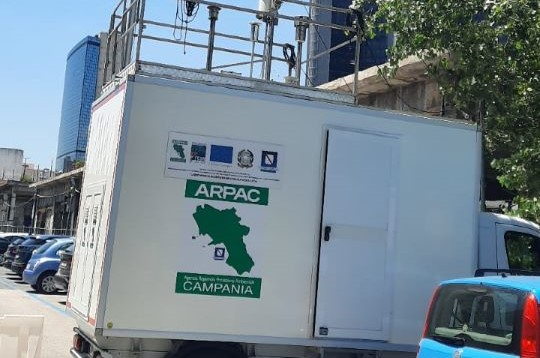
\includegraphics[width=0.6\textwidth]{images/ARPAC STAZIONE.jpg}
    \caption{Esempio di stazione di monitoraggio.}
    \label{fig:arpac_stazione}
\end{figure}

% ------------------------------------------------------------
\section{Il dataset}
\label{sec:arpac}

I dati provengono dal portale Open Data di ARPA Campania \cite{arpac}, che
pubblica mensilmente le misure orarie di tutte le stazioni della rete regionale
di monitoraggio della qualità dell'aria. Abbiamo scelto questa fonte perché
offre dati reali, recenti e pubblicati da un ente istituzionale, con una
frequenza di misura (oraria) e una durata (oltre tre anni) adatte sia
all'analisi delle serie temporali sia alle tecniche di classificazione e di
clustering.

Il portale mette a disposizione due versioni dei dati: i dati \emph{grezzi}
(\emph{near real time}), pubblicati quasi in tempo reale, e i dati
\emph{validati}, sottoposti ai controlli di qualità dell'agenzia.
Abbiamo scelto i dati validati, più affidabili, tenendo conto di
qualche lacune nella valutazione della continuità dei dati
(Sezione~\ref{sec:continuita}).

I 44 file mensili, da marzo 2023 a ottobre 2026, sono stati scaricati il
29/10/2026 e concatenati in un unico file. La Tabella~\ref{tab:arpac} ne
riassume le caratteristiche.

\begin{table}[H]
  \centering
  \caption{Caratteristiche del dataset utilizzato.}
  \label{tab:arpac}
  \begin{tabular}{ll}
    \toprule
    Fonte              & Portale Open Data ARPA Campania \cite{arpac}                             \\
    Dataset            & \emph{Dati RQA Orari Validati}                                           \\
    Licenza            & CC BY 4.0                                                                \\
    Periodo            & 20/03/2023 -- 26/10/2026                                                 \\
    File               & 44 file mensili CSV, concatenati in un unico file (\SI{395}{\mega\byte}) \\
    Data del download  & 29/10/2026                                                               \\
    Righe              & \num{4905168}                                                            \\
    Codici di stazione & 57                                                                       \\
    Inquinanti         & 7                                                                        \\
    \bottomrule
  \end{tabular}
\end{table}

% ------------------------------------------------------------
\section{Struttura dei dati}
\label{sec:struttura}

I dati sono organizzati in formato \emph{lungo}: ogni riga corrisponde alla
misura di un inquinante, in una stazione, in una determinata ora. La
Tabella~\ref{tab:colonne} descrive le sette colonne del file.

\begin{table}[H]
  \centering
  \caption{Colonne del dataset originale.}
  \label{tab:colonne}
  \begin{tabularx}{\textwidth}{l l >{\raggedright\arraybackslash}X l}
    \toprule
    \textbf{Colonna}     & \textbf{Tipo} & \textbf{Descrizione}                   & \textbf{Esempio}           \\
    \midrule
    \texttt{\_id}        & intero        & numero di riga interno al file mensile & 1                          \\
    \texttt{Stazione}    & testo         & codice europeo (EEA) della stazione    & IT2211A                    \\
    \texttt{Descrizione} & testo         & nome della stazione                    & Acerra Zona Industriale    \\
    \texttt{Inquinante}  & testo         & inquinante misurato                    & PM10                       \\
    \texttt{Data\_ora}   & testo         & data, ora e fuso orario                & 01-09-2023 00:00:00 +01:00 \\
    \texttt{Valore}      & testo         & concentrazione misurata                & 27.1                       \\
    \texttt{Um}          & testo         & unità di misura                        & \ugm                       \\
    \bottomrule
  \end{tabularx}
\end{table}

Il codice della stazione segue la nomenclatura dell'Agenzia europea
dell'ambiente (EEA): le stazioni fisse della rete hanno codici della forma
\texttt{IT}, seguito da quattro cifre e dalla lettera \texttt{A}. Il nome della
stazione indica in genere il comune e il luogo di installazione (una scuola, un
parco, una zona industriale).

\subsection{Gli inquinanti}

Il dataset contiene le misure di sette inquinanti:
\begin{itemize}
  \item \textbf{PM10 e PM2,5}: particelle sospese con diametro inferiore
        rispettivamente a \SI{10}{\micro\metre} e a \SI{2,5}{\micro\metre}.
        \textbf{Derivano dal traffico} (gas di scarico, ma anche usura di freni,
        pneumatici e asfalto), dal riscaldamento domestico, dall'industria e
        da fonti naturali come la sabbia sahariana. Le PM2,5, più fini,
        penetrano più in profondità nell'apparato respiratorio;
  \item \textbf{NO\textsubscript{2}} (biossido di azoto): gas prodotto dai
        processi di combustione, in ambito urbano soprattutto dal traffico
        veicolare;
  \item \textbf{O\textsubscript{3}} (ozono): inquinante \emph{secondario}, non
        emesso direttamente ma formato in atmosfera per effetto della radiazione
        solare a partire da altri inquinanti; raggiunge per questo i valori più
        alti in estate;
  \item \textbf{CO} (monossido di carbonio): gas prodotto dalla combustione
        incompleta, in particolare dei motori dei veicoli;
  \item \textbf{SO\textsubscript{2}} (biossido di zolfo): gas legato alla
        combustione di combustibili contenenti zolfo, in ambito industriale e
        portuale;
  \item \textbf{C\textsubscript{6}H\textsubscript{6}} (benzene): composto
        organico cancerogeno, emesso principalmente dai carburanti e dal
        traffico.
\end{itemize}

\subsection{I valori limite}

La Direttiva 2008/50/CE \cite{direttiva}, recepita in Italia dal D.Lgs.\
155/2010, fissa per ogni inquinante dei \emph{valori limite}: una
concentrazione da non superare, calcolata come media su un determinato
\emph{periodo di mediazione} (un'ora, un giorno, otto ore o un anno). Per
alcuni limiti è consentito un numero massimo di superamenti per anno civile: ad
esempio, la media giornaliera del PM10 può superare
\SI{50}{\micro\gram\per\cubic\metre} al massimo 35 volte all'anno. Per l'ozono
la norma fissa invece un \emph{valore obiettivo}, cioè un livello da
raggiungere, meno vincolante di un valore limite. La
Tabella~\ref{tab:inquinanti} riporta, per ogni inquinante, l'unità di misura,
il numero di misure presenti nel dataset e i principali limiti di legge. Questi
valori costituiscono un riferimento per interpretare le concentrazioni misurate
e definiscono la variabile da prevedere nel capitolo di classificazione. La
nuova Direttiva (UE) 2024/2881 prevede limiti più stringenti a partire dal 2030
\cite{direttiva2024}.

\begin{table}[H]
  \centering
  \caption{Inquinanti presenti nel dataset e principali valori limite (Direttiva 2008/50/CE).}
  \label{tab:inquinanti}
  \small
  \begin{tabularx}{\textwidth}{l l r >{\raggedright\arraybackslash}X r r}
    \toprule
    \textbf{Inquinante}                  & \textbf{Unità} & \textbf{Misure} & \textbf{Periodo di mediazione} & \textbf{Limite}        & \textbf{Superamenti/anno} \\
    \midrule
    NO\textsubscript{2}                  & \ugm           & \num{995793}    & 1 ora                          & 200                    & 18                        \\
                                         &                &                 & anno civile                    & 40                     & --                        \\
    PM10                                 & \ugm           & \num{894611}    & 24 ore                         & 50                     & 35                        \\
                                         &                &                 & anno civile                    & 40                     & --                        \\
    PM2,5                                & \ugm           & \num{890014}    & anno civile                    & 25                     & --                        \\
    C\textsubscript{6}H\textsubscript{6} & \ugm           & \num{627446}    & anno civile                    & 5                      & --                        \\
    O\textsubscript{3}                   & \ugm           & \num{562616}    & massima media mobile su 8 ore  & 120\textsuperscript{*} & 25\textsuperscript{**}    \\
    CO                                   & \mgm           & \num{558442}    & massima media mobile su 8 ore  & 10                     & --                        \\
    SO\textsubscript{2}                  & \ugm           & \num{376246}    & 1 ora                          & 350                    & 24                        \\
                                         &                &                 & 24 ore                         & 125                    & 3                         \\
    \bottomrule
    \multicolumn{6}{l}{\footnotesize \textsuperscript{*} Valore obiettivo. \textsuperscript{**} Media su tre anni.}
  \end{tabularx}
\end{table}

% ------------------------------------------------------------
\section{Pre-processing}
\label{sec:preprocessing}

L'obiettivo del pre-processing è fornire ai capitoli successivi dati puliti e
affidabili, documentando ogni scelta effettuata. Le operazioni sono state
svolte in Python con la libreria pandas, in un notebook Jupyter dedicato.

\subsection{Colonne eliminate}
La colonna \texttt{\_id} è stata eliminata: non identifica le misure, ma è un
numero di riga interno a ciascun file mensile, che riparte da 1 ogni mese. Nel
file concatenato assume infatti solo \num{140415} valori distinti su
\num{4905168} righe, esattamente il numero di righe del file più grande, quello
di luglio 2026.

La colonna \texttt{Um} è costante per ogni inquinante: tutte le concentrazioni
sono espresse in \ugm, \textbf{tranne quelle del CO, espresse in \mgm (un milligrammo
equivale a mille microgrammi)}. La colonna è stata mantenuta per completezza.
Questa differenza va considerata quando si confrontano gli inquinanti tra loro:
i valori del CO risultano numericamente molto più piccoli degli altri.

\subsection{Conversione delle date}
Il controllo della colonna \texttt{Data\_ora} ha rivelato la presenza di due
formati diversi (Tabella~\ref{tab:formati_date}), il secondo formato riguarda solo le
misure dal 7 al 10 ottobre 2025, probabilmente a causa di un cambiamento
temporaneo nel sistema di pubblicazione dell'agenzia.

\begin{table}[H]
  \centering
  \caption{Formati della colonna \texttt{Data\_ora}.}
  \label{tab:formati_date}
  \begin{tabular}{l l r}
    \toprule
    \textbf{Formato}                    & \textbf{Esempio}           & \textbf{Righe} \\
    \midrule
    \texttt{gg-mm-aaaa hh:mm:ss +01:00} & 26-10-2026 23:00:00 +01:00 & \num{4881186}  \\
    \texttt{aaaa-mm-gg hh:mm:ss+01}     & 2025-10-07 01:00:00+01     & \num{23982}    \\
    \bottomrule
  \end{tabular}
\end{table}

Lasciare che pandas riconosca automaticamente il formato avrebbe portato a
convertire correttamente solo una parte delle date. Abbiamo quindi letto i due
formati in modo esplicito, indicando a pandas la struttura di ciascuno, e unito
i risultati, tutte le date sono state convertite in datetime.

Tutte le misure riportano lo stesso fuso orario (UTC+1), le date sono state quindi
espresse in ora fissa UTC+1, senza passaggio all'ora legale dunque abbiamo deciso che l'indicazione
del fuso doveva essere rimossa. Il periodo coperto va \textbf{dal 20/03/2023 alle 00:00 al
26/10/2026 alle 23:00}.

\paragraph{}
\textbf{NOTA :} La documentazione di ARPAC non specifica se l'orario indichi l'inizio o la fine
dell'intervallo di misura. Poiché ogni file mensile inizia alle 00:00 del primo
giorno del mese, abbiamo assunto che l'orario indichi l'inizio dell'intervallo,
senza applicare correzioni. Segnaliamo tuttavia che il 31/03/2024, giorno del
passaggio all'ora legale, alcune stazioni presentano solo 23 ore di misure: ciò
suggerisce che gli orari possano seguire in realtà l'ora locale italiana,
nonostante l'indicazione UTC+1.

\subsection{Valori mancanti codificati}
Il dataset non contiene celle vuote, ma questo non significa che sia completo,
per due motivi.

In primo luogo, le ore in cui una stazione non ha misurato un
inquinante non compaiono affatto nel file, l'assenza di una misura corrisponde
all'assenza di una riga. 

In secondo luogo, una volta convertiti in numeri, i
valori della colonna \texttt{Valore} hanno rivelato misure non valide
codificate con valori negativi:
\begin{itemize}
  \item \num{202303} valori pari a $-9999$ (circa il 4\% delle righe), codice
        convenzionale di valore mancante;
  \item 224 altri valori negativi, fisicamente impossibili per una
        concentrazione: in parte piccoli valori vicini allo zero, dovuti al
        rumore degli strumenti, in parte valori chiaramente errati (fino a
        \SI{-104,1}{\micro\gram\per\cubic\metre} per l'O\textsubscript{3}).
\end{itemize}
Lasciati nel dataset, questi valori avrebbero falsato qualsiasi media,\textbf{ un solo
$-9999$ in una giornata basterebbe a rendere fortemente negativa la media
giornaliera}. I \num{202527} valori negativi sono stati quindi sostituiti con
\texttt{NaN}, il valore mancante di pandas, che viene ignorato automaticamente
nel calcolo delle medie. Le righe sono state invece conservate, per non
interrompere la struttura delle serie temporali.

\subsection{Esclusione delle stazioni}
Dei 57 codici di stazione presenti, 21 non sono adatti alle analisi del
progetto (Tabella~\ref{tab:stazioni_escluse}).

\begin{table}[H]
  \centering
  \caption{Stazioni escluse dall'analisi.}
  \label{tab:stazioni_escluse}
  \begin{tabularx}{\textwidth}{>{\raggedright\arraybackslash}X >{\raggedright\arraybackslash}X}
    \toprule
    \textbf{Stazioni}                  & \textbf{Motivo}                                                          \\
    \midrule
    Laboratori mobili (LM01, LM03, MMA61, MMB62), impianti STIR, EDI01, EDI02
                                       & stazioni non fisse, presenti solo dal 7 al 18 ottobre 2025               \\
    IT2220A, IT2222A, IT2224A, IT2225A, IT2342A
                                       & installate a marzo 2026: circa 7 mesi di dati, senza un inverno completo \\
    IT2269A (Salerno Parco Mercatello) & dismessa ad agosto 2023, meno di 5 mesi di dati                          \\
    \bottomrule
  \end{tabularx}
\end{table}

Le stazioni installate nel 2026 meritano una precisione. Le loro misure non
sono errate e, nel periodo marzo-ottobre 2026, sono confrontabili con quelle
delle altre stazioni. Tuttavia, poiché gli inquinanti hanno un forte andamento
stagionale (il particolato e l'NO\textsubscript{2} raggiungono i valori massimi
in inverno, l'ozono in estate), stazioni prive di dati invernali avrebbero
medie non confrontabili con quelle delle stazioni attive per più anni. Abbiamo
escluso anche la stazione IT2269A, dismessa dopo pochi mesi, e mantenuto invece
la stazione IT2272A (Pozzuoli), attiva da giugno 2024: la scelta di includerla
o meno è lasciata ai singoli capitoli, in base al periodo analizzato.

L'esclusione ha eliminato \num{134842} righe; restano \textbf{36 stazioni}.

\subsection{Valori anomali}
I valori massimi di alcuni inquinanti sono risultati del tutto irrealistici:
fino a \num{1437008} \ugm per il PM10, mentre anche gli episodi di inquinamento
più intensi raramente superano poche centinaia di \ugm. Non abbiamo però
applicato una soglia automatica, perché alcuni valori estremi corrispondono a
fenomeni reali. Per ogni valore sospetto abbiamo invece osservato il contesto,
cioè le misure delle ore precedenti e successive nella stessa stazione:
\begin{itemize}
  \item un valore \emph{isolato}, circondato da valori normali o mancanti, è stato
        considerato un errore di misura;
  \item un picco con una salita e una discesa graduali, distribuite su più ore, è stato
        considerato un episodio reale di inquinamento.
\end{itemize}

I quattro valori della Tabella~\ref{tab:anomali} sono stati sostituiti con
\texttt{NaN}. In tutti i casi il valore anomalo compare isolato, tra ore senza
misure o con valori normali, ad esempio il valore di \num{1437008} \ugm della
stazione IT1504A è l'unica misura di una mattinata in cui lo strumento registra
solo $-9999$, mentre il PM2,5 della stazione IT0934A passa da circa
\SI{20}{\micro\gram\per\cubic\metre} a \num{17792,5} e poi a \num{101090} \ugm,
per tornare a valori normali nel pomeriggio.

\begin{table}[H]
  \centering
  \caption{Valori anomali sostituiti con \texttt{NaN}.}
  \label{tab:anomali}
  \begin{tabular}{l l l r}
    \toprule
    \textbf{Stazione} & \textbf{Inquinante} & \textbf{Data e ora} & \textbf{Valore (\ugm)} \\
    \midrule
    IT1504A           & PM10                & 01/09/2023 09:00    & \num{1437008}          \\
    IT1493A           & NO\textsubscript{2} & 22/11/2024 23:00    & \num{4992.6}           \\
    IT0934A           & PM2,5               & 13/06/2025 10:00    & \num{17792.5}          \\
    IT0934A           & PM2,5               & 13/06/2025 12:00    & \num{101090}           \\
    \bottomrule
  \end{tabular}
\end{table}

Al contrario, il picco di PM10 registrato a Napoli nella notte di Capodanno
(stazione IT0898A) è stato conservato, la concentrazione sale nel corso della
serata, raggiunge \SI{2721,9}{\micro\gram\per\cubic\metre} all'01:00 del
01/01/2025 e torna gradualmente ai valori abituali nel corso della mattinata.
Si tratta dell'effetto dei fuochi d'artificio. Anche i valori elevati del PM10 alla stazione
IT2226A intorno a mezzogiorno del 01/01/2026 sono stati conservati.

\paragraph{}
\textbf{NOTA :} Segnaliamo infine la stazione IT1486A, che tra agosto e settembre 2024 registra
per alcune giornate intere un valore di PM10 costante e molto elevato (tra
\num{1596} e \num{2453} \ugm). \textbf{Questi valori non sono stati modificati, ma
vanno considerati con cautela nelle analisi}.

\subsection{Il particolato su base giornaliera}
Cercando eventuali strumenti bloccati, abbiamo contato le giornate in cui una
stazione registra lo stesso valore per tutte le ore disponibili (almeno 18). Il
risultato varia molto da un inquinante all'altro: \num{5965} giornate per il
PM10 e \num{6164} per il PM2,5, contro 2 per l'NO\textsubscript{2} e 2 per
l'O\textsubscript{3} (e alcune centinaia per CO, SO\textsubscript{2} e benzene,
i cui valori sono spesso bassi e misurati con una precisione limitata). Se si
trattasse di guasti, colpirebbero tutti gli inquinanti in modo simile. \textbf{La
spiegazione più probabile è invece il metodo di misura, sicuramente in molte stazioni il
particolato viene misurato su base giornaliera, raccogliendo le particelle su
un filtro per 24 ore, e il valore giornaliero viene poi ripetuto per tutte le
ore della giornata}.

Queste giornate costanti sono quindi misure valide e sono state conservate. Ne
segue però che, per queste stazioni, il PM10 e il PM2,5 non hanno un vero
profilo orario: \textbf{il particolato verrà analizzato a scala giornaliera}.

\subsection{Dataset finale}
Il dataset pulito è stato salvato in formato Parquet, più compatto e veloce da
leggere di un file CSV, che conserva inoltre i tipi delle colonne (date e
numeri). Le sue caratteristiche sono:
\begin{itemize}
  \item file \texttt{data/processed/aria\_campania\_orario.parquet}, in formato lungo e
        a frequenza oraria;
        % verificare il numero di righe con len(df) nel notebook
  \item \num{4770326} righe, 36 stazioni, 7 inquinanti;
  \item colonne \texttt{Stazione}, \texttt{Descrizione}, \texttt{Inquinante},
        \texttt{Data\_ora}, \texttt{Valore}, \texttt{Um};
  \item periodo dal 20/03/2023 al 26/10/2026.
\end{itemize}
Per identificare le stazioni va usato il codice (\texttt{Stazione}) e non il
nome, la colonna \texttt{Descrizione} riporta infatti nomi diversi per la
stessa stazione a seconda del mese (ad esempio ``Casoria Scuola Palizzi'' e
``Casoria Scuola Palizzi (CAM)'').

% ------------------------------------------------------------
\section{Qualità e continuità dei dati}
\label{sec:continuita}

La Figura~\ref{fig:completezza} mostra, per ogni stazione e ogni mese, la quota
di giorni in cui è disponibile almeno una misura di PM10. La figura è stata
prodotta prima dell'esclusione delle stazioni e include quindi anche le
stazioni escluse, visibili come righe quasi interamente rosse.

\begin{figure}[!h]
    \centering
    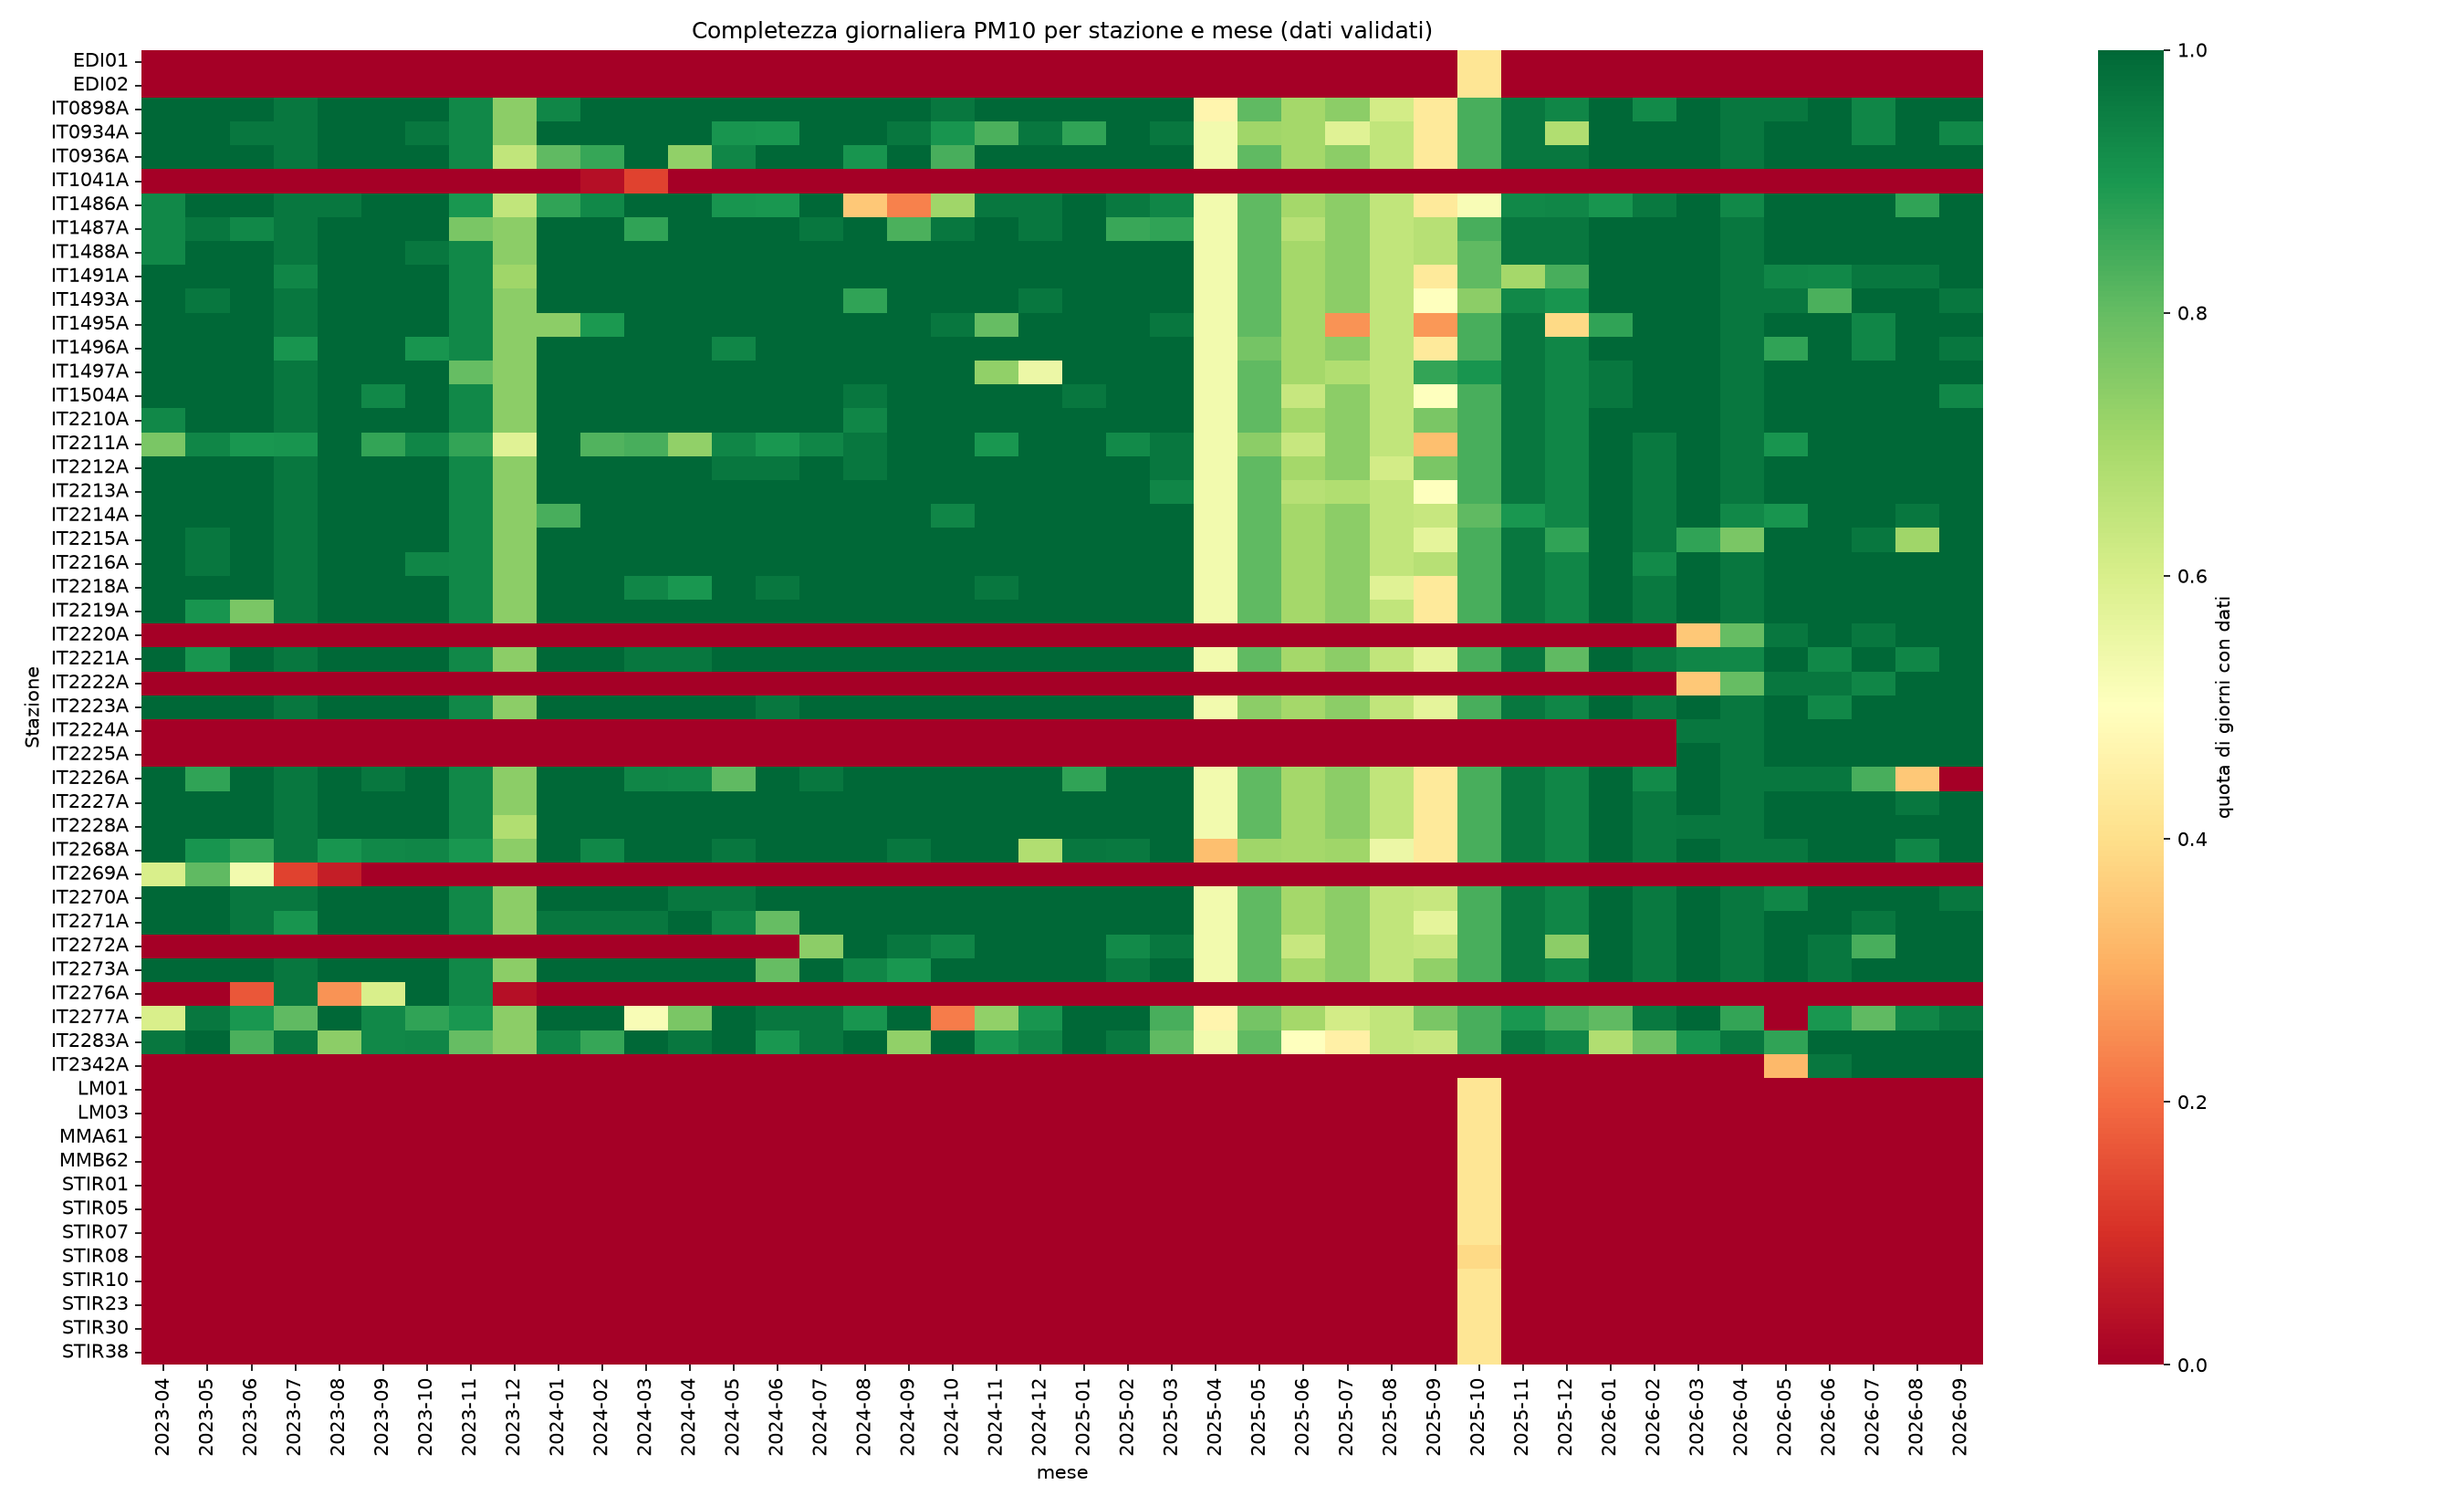
\includegraphics[width=1.0\textwidth]{completezza_pm10.png}
    \caption{Completezza giornaliera del PM10 per stazione e mese.}
    \label{fig:completezza}
\end{figure}

Per la maggior parte delle stazioni la copertura è molto buona, 31 stazioni
hanno dati di PM10 per l'86-94\% dei giorni. Le lacune più evidenti (dicembre
2023, aprile 2025 e il periodo maggio-ottobre 2025) colpiscono tutte le
stazioni contemporaneamente, non sono quindi dovute a guasti dei singoli
strumenti, ma alla pubblicazione o alla validazione dei dati da parte
dell'agenzia. Per questo motivo non possono essere colmate con le misure delle
stazioni vicine.

\textbf{IMPORTANTE :} Non tutte le stazioni misurano tutti gli inquinanti. La
Tabella~\ref{tab:copertura} riporta, per ogni inquinante, il numero di stazioni
con dati disponibili per almeno l'80\% dei giorni: il NO\textsubscript{2} e i
particolati PM sono misurati in quasi tutte le stazioni, mentre l'ozono e
soprattutto il biossido di zolfo solo in una parte della rete.

\begin{table}[H]
  \centering
  \caption{Stazioni con almeno l'80\% dei giorni con dati (aprile 2023 -- settembre 2026).}
  \label{tab:copertura}
  \begin{tabular}{l c c c c c c c}
    \toprule
             & NO\textsubscript{2} & PM10 & PM2,5 & C\textsubscript{6}H\textsubscript{6} & CO & O\textsubscript{3} & SO\textsubscript{2} \\
    \midrule
    Stazioni & 35                  & 32   & 32    & 23                                   & 20 & 19                 & 13                  \\
    \bottomrule
  \end{tabular}
\end{table}

Per l'analisi delle serie temporali, la continuità del periodo aprile 2023 --
marzo 2025 è buona, mancano solo 11 giorni su 731 (1,5\%) in cui nessuna
stazione ha misurato il PM10, con al massimo 3 giorni consecutivi (21--23
dicembre 2023). Si tratta di lacune brevi, che possono essere colmate per
interpolazione.

% ============================================================
%  CAPITOLO 2 - ANALISI DESCRITTIVA
% ============================================================
\chapter{Analisi descrittiva}
\label{cap:descrittiva}

% ------------------------------------------------------------
\section{Introduzione}
\label{sec:intro_descrittiva}

Questo capitolo esplora i dati puliti ottenuti con il pre-processing
(Capitolo~\ref{cap:dataset}), con l'obiettivo di descrivere le distribuzioni
degli inquinanti, il loro andamento nel tempo, le differenze tra le stazioni e le
relazioni tra inquinanti.

\subsection{Librerie utilizzate}
L'analisi è stata svolta in Python, in un notebook Jupyter dedicato, con le
seguenti librerie:
\begin{itemize}
  \item \textbf{pandas}: lettura del dataset in formato Parquet, filtri,
        raggruppamenti e calcolo delle medie giornaliere, mensili e orarie;
  \item \textbf{NumPy}: operazioni numeriche e gestione dei valori mancanti;
  \item \textbf{Matplotlib} e \textbf{Seaborn}: realizzazione dei grafici
        (boxplot, serie temporali, grafici a barre e mappe di calore);
  \item \textbf{SciPy}: utilizzata da pandas per il calcolo della correlazione
        di Spearman.
\end{itemize}

\subsection{Scala temporale}
La maggior parte delle analisi utilizza le \emph{medie giornaliere} di ciascun
inquinante in ciascuna stazione. Questa è la scala dei valori limite giornalieri ed
è l'unica significativa per il particolato, il cui valore in molte stazioni è
giornaliero e ripetuto su tutte le ore (Sezione~\ref{sec:preprocessing}). Seguendo
il criterio adottato dalla normativa europea, una media giornaliera è considerata
valida solo se calcolata su almeno 18 ore di misure (75\% della giornata). Solo il
profilo orario (Sezione~\ref{sec:temporale}) utilizza i dati orari, e solo per i gas.

Nei grafici che mostrano l'andamento complessivo della regione si utilizza la
\emph{media di rete}, cioè la media delle medie giornaliere di tutte le stazioni
disponibili in un determinato giorno. Poiché il numero di stazioni attive varia
leggermente nel tempo (guasti, attivazione della stazione IT2272A a giugno 2024),
la media di rete non è calcolata ogni giorno esattamente sulle stesse stazioni; ciò
non altera tuttavia la lettura degli andamenti generali.

% ------------------------------------------------------------
\section{Statistiche descrittive per inquinante}
\label{sec:statistiche}

\begin{table}[H]
  \centering
  \caption{Statistiche descrittive delle medie giornaliere per inquinante (\ugm, CO in \mgm).}
  \label{tab:describe}
  \small
  \begin{tabular}{l r r r r r r r r}
    \toprule
    \textbf{Inquinante} & \textbf{N} & \textbf{Media} & \textbf{Dev.\ std.} & \textbf{Min} & \textbf{25\%} & \textbf{Mediana} & \textbf{75\%} & \textbf{Max} \\
    \midrule
    PM10 & \num{35057} & \num{26.1} & \num{30.2} & \num{0.0} & \num{14.8} & \num{21.8} & \num{31.4} & \num{2453.0} \\
    PM2,5 & \num{35186} & \num{13.9} & \num{12.0} & \num{0.0} & \num{7.5} & \num{11.4} & \num{16.8} & \num{345.0} \\
    NO\textsubscript{2} & \num{38913} & \num{23.0} & \num{14.8} & \num{0.0} & \num{12.1} & \num{20.3} & \num{31.0} & \num{212.9} \\
    O\textsubscript{3} & \num{21635} & \num{56.1} & \num{23.0} & \num{0.0} & \num{39.7} & \num{56.5} & \num{71.6} & \num{529.0} \\
    CO & \num{21678} & \num{0.5} & \num{0.3} & \num{0.0} & \num{0.3} & \num{0.4} & \num{0.6} & \num{18.4} \\
    SO\textsubscript{2} & \num{14392} & \num{2.8} & \num{3.5} & \num{0.0} & \num{1.0} & \num{2.2} & \num{3.7} & \num{289.5} \\
    C\textsubscript{6}H\textsubscript{6} & \num{24309} & \num{1.0} & \num{1.0} & \num{0.0} & \num{0.4} & \num{0.7} & \num{1.2} & \num{22.2} \\
    \bottomrule
  \end{tabular}
\end{table}

Le colonne della Tabella~\ref{tab:describe} hanno il seguente significato:
\begin{itemize}
  \item \textbf{N}: numero di medie giornaliere valide (coppie stazione-giorno);
  \item \textbf{Media}: media aritmetica delle medie giornaliere;
  \item \textbf{Dev.\ std.}: deviazione standard, che misura quanto i valori si
        discostano in media dalla media: più è alta, più le concentrazioni sono variabili;
  \item \textbf{Min} e \textbf{Max}: valore minimo e massimo osservati;
  \item \textbf{25\%}: primo quartile, cioè il valore al di sotto del quale si
        trova il 25\% delle giornate;
  \item \textbf{Mediana}: valore che divide le giornate in due metà uguali
        (il 50\% delle giornate ha un valore inferiore, il 50\% superiore); a
        differenza della media, non è influenzata dai valori estremi;
  \item \textbf{75\%}: terzo quartile, cioè il valore al di sotto del quale si
        trova il 75\% delle giornate.
\end{itemize}
Quando la media è nettamente superiore alla mediana, la distribuzione è
asimmetrica a destra: la maggior parte delle giornate presenta valori bassi, ma
alcune giornate con valori molto elevati alzano la media.

Il numero di medie giornaliere varia molto tra gli inquinanti, poiché non tutte le
stazioni li misurano tutti: da \num{38913} per l'NO\textsubscript{2}, misurato in
quasi tutta la rete, a \num{14392} per l'SO\textsubscript{2}. Per tutti gli
inquinanti la media è superiore alla mediana, segno di distribuzioni asimmetriche a
destra. Il caso più evidente è il PM10: la media (\SI{26,1}{\micro\gram\per\cubic\metre})
supera la mediana (\SI{21,8}{\micro\gram\per\cubic\metre}) e la deviazione standard
(\num{30,2}) è superiore alla media stessa, per effetto di pochi valori estremi,
come le giornate anomale della stazione IT1486A, che determinano il massimo di
\num{2453} \ugm. Al contrario, l'intervallo tra primo e terzo quartile, da 14,8 a
\SI{31,4}{\micro\gram\per\cubic\metre}, descrive bene le giornate abituali.

Alcuni valori massimi appaiono poco plausibili anche come medie giornaliere, \textbf{in
particolare \SI{529}{\micro\gram\per\cubic\metre} per l'ozono e
\SI{289,5}{\micro\gram\per\cubic\metre} per l'SO\textsubscript{2}}. Questi valori, non individuati durante il pre-processing,
riguardano un numero molto limitato di giornate e non modificano mediane e quartili,
ma vanno tenuti presenti nei capitoli successivi.

% ------------------------------------------------------------
\section{Distribuzione dei valori}
\label{sec:distribuzioni}

\figura{distribuzione_inquinanti.png}{Distribuzione delle medie giornaliere per inquinante (CO escluso, perché misurato in \mgm; valori estremi non rappresentati).}{fig:distribuzioni}

La Figura~\ref{fig:distribuzioni} confronta le distribuzioni delle medie
giornaliere tramite boxplot: la linea interna a ciascun rettangolo indica la
mediana, \textbf{il rettangolo contiene il 50\% centrale delle giornate (dal primo al terzo
quartile)} e i segmenti si estendono fino ai valori più lontani non considerati
estremi. Per leggibilità, i valori estremi non sono rappresentati; il CO è escluso
perché misurato in un'unità diversa (\mgm).

L'ozono presenta le concentrazioni più elevate (mediana di circa
\SI{56}{\micro\gram\per\cubic\metre}, con metà delle giornate tra 40 e
\SI{72}{\micro\gram\per\cubic\metre}) e la dispersione maggiore, coerente con la
sua forte stagionalità (Sezione~\ref{sec:temporale}). L'NO\textsubscript{2} e il
PM10 hanno livelli simili, con mediane intorno a 20--\SI{22}{\micro\gram\per\cubic\metre};
il segmento superiore del PM10 supera il limite giornaliero di
\SI{50}{\micro\gram\per\cubic\metre}, ma oltre il terzo quartile (circa
\SI{31}{\micro\gram\per\cubic\metre}), i superamenti riguardano quindi una minoranza
di giornate. Questa informazione è rilevante per la classificazione, perché le due
classi (superamento e non superamento) risulteranno sbilanciate. Il PM2,5 vale circa
la metà del PM10 (mediana di circa \SI{11}{\micro\gram\per\cubic\metre}), mentre
l'SO\textsubscript{2} e il benzene restano su valori molto bassi, lontani dai
rispettivi limiti.

% ------------------------------------------------------------
\section{Andamento temporale}
\label{sec:temporale}

\subsection{Andamento complessivo 2023--2026}

\figura{andamento_temporale.png}{Media giornaliera di rete di PM10, NO\textsubscript{2} e O\textsubscript{3} (in grigio) e media mobile centrata a 7 giorni.}{fig:andamento}

La Figura~\ref{fig:andamento} mostra la media giornaliera di rete di PM10,
NO\textsubscript{2} e O\textsubscript{3}. Per rendere leggibile l'andamento di
lungo periodo, ai valori giornalieri (in grigio) è sovrapposta la media mobile
centrata a 7 giorni, in cui ogni giorno è sostituito dalla media dei sette giorni
che lo circondano, questa attenua le fluttuazioni giornaliere e il ciclo
settimanale, \textbf{mettendo in evidenza le variazioni stagionali. I giorni mancanti non
sono interpolati, così che le lacune dei dati restino visibili}.

L'ozono (Troposfera: l'ozono "inquinante") presenta una stagionalità molto marcata e regolare, raggiunge
70--\SI{80}{\micro\gram\per\cubic\metre} in estate e scende intorno a
\SI{30}{\micro\gram\per\cubic\metre} in inverno, per effetto della radiazione
solare che ne favorisce la formazione. L'NO\textsubscript{2} segue l'andamento
opposto, con valori massimi in inverno (35--\SI{40}{\micro\gram\per\cubic\metre})
e minimi in estate.

Il PM10 mostra una stagionalità meno evidente, i valori abituali restano tra 15 e
\SI{35}{\micro\gram\per\cubic\metre}, ma emergono alcuni episodi intensi, tra cui
l'evento dell'inizio di aprile 2024 e le notti di Capodanno del 2025 e del 2026
(Sezione~\ref{sec:eventi}). La media di rete supera il limite giornaliero di
\SI{50}{\micro\gram\per\cubic\metre} solo durante questi episodi, mentre singole
stazioni possono superarlo anche quando la media di rete resta inferiore.

Il grafico rende visibili anche le lacune della rete descritte nella
Sezione~\ref{sec:continuita}, in particolare il periodo frammentato tra aprile e
ottobre 2025. Il periodo aprile 2023 -- marzo 2025 si conferma il più continuo.

\subsection{Stagionalità}

\figura{stagionalita_mensile.png}{Concentrazione media di PM10, PM2,5, NO\textsubscript{2} e O\textsubscript{3} per mese dell'anno.}{fig:stagionalita}

La Figura~\ref{fig:stagionalita} riporta la concentrazione media di ciascun
inquinante per mese dell'anno, raggruppando gli stessi mesi di anni diversi.
L'ozono raggiunge i valori massimi in luglio e agosto (circa
\SI{68}{\micro\gram\per\cubic\metre}) e i minimi in dicembre (circa
\SI{37}{\micro\gram\per\cubic\metre}), quasi dimezzandosi. L'NO\textsubscript{2}
segue l'andamento opposto, con il massimo in dicembre (circa
\SI{29}{\micro\gram\per\cubic\metre}) e i minimi in maggio e agosto (circa
\SI{19}{\micro\gram\per\cubic\metre}), in inverno la maggiore stabilità
dell'atmosfera, con frequenti inversioni termiche, ostacola la dispersione degli
inquinanti, mentre in estate parte dell'NO\textsubscript{2} è consumata nella
formazione dell'ozono.

Il PM2,5 è nettamente più elevato in inverno (circa
\SI{24}{\micro\gram\per\cubic\metre} in dicembre, contro
\SI{9}{\micro\gram\per\cubic\metre} in maggio), \textbf{in coerenza con il contributo della
combustione e del riscaldamento domestico}. Il PM10 presenta invece due massimi: uno
invernale, analogo a quello del PM2,5, e uno estivo, in luglio e agosto, assente nel
PM2,5. Il rapporto PM2,5/PM10 scende infatti da circa 0,7 in dicembre a circa 0,5
nei mesi estivi, in estate prevalgono le particelle più grossolane, tra
\SI{2,5}{} e \SI{10}{\micro\metre}, riconducibili \textbf{ad esempio alle polveri sahariane,
alla risospensione del suolo secco e al sale marino}.

Va osservato che i mesi non sono rappresentati in modo uniforme: i dati iniziano a
marzo 2023, terminano a ottobre 2026 e presentano ampie lacune tra aprile e ottobre
2025. Alcuni mesi, come dicembre, sono quindi rappresentati da un numero limitato di
anni, e un singolo episodio intenso può influenzarne sensibilmente la media.

\subsection{Ciclo settimanale}

\figura{ciclo_settimanale.png}{Scarto percentuale della concentrazione media di ciascun giorno della settimana rispetto alla media settimanale.}{fig:settimanale}

La Figura~\ref{fig:settimanale} riporta, per ogni inquinante, lo scarto percentuale
della concentrazione media di ciascun giorno della settimana rispetto alla media
settimanale; questa rappresentazione permette di confrontare inquinanti con livelli
e unità di misura diversi. Gli inquinanti legati al traffico mostrano un netto calo
nel fine settimana, la domenica l'NO\textsubscript{2} è inferiore alla media di
circa il 15\%, il benzene di circa il 13\% e il CO di circa il 6\%, mentre nei
giorni feriali restano al di sopra della media, con i valori più alti tra giovedì e
venerdì. Anche il PM10 diminuisce la domenica (circa $-10$\%), a \textbf{conferma del
contributo del traffico al particolato (emissioni dei veicoli, usura di freni e
pneumatici, risospensione delle polveri stradali)}.

L'ozono segue l'andamento opposto, con valori inferiori alla media nei giorni
feriali e superiori nel fine settimana (circa $+3{,}5$\% la domenica). con meno
traffico.

\textbf{In ambito urbano viene consumato meno ozono dalle emissioni dei veicoli
(``effetto weekend'')}.

\subsection{Ciclo giornaliero}

\figura{ciclo_giornaliero.png}{Profilo orario medio di NO\textsubscript{2}, O\textsubscript{3}, CO e benzene, espresso come scarto percentuale dalla media giornaliera.}{fig:giornaliero}

La Figura~\ref{fig:giornaliero} mostra il profilo orario medio dei gas, espresso
come scarto percentuale dalla media giornaliera. Il particolato è escluso da questa
analisi, poiché in molte stazioni il suo valore è giornaliero e ripetuto su tutte
le ore.

L'NO\textsubscript{2}, il CO e il benzene presentano due massimi, in corrispondenza
delle ore di punta del traffico, il primo al mattino, intorno alle 7--8 (circa
$+29$\% per l'NO\textsubscript{2}), il secondo, più intenso, in serata, tra le 19 e
le 21 (circa $+36$\% per l'NO\textsubscript{2} e $+39$\% per il benzene).

L'ozono segue un andamento opposto: è minimo all'alba (circa $-31$\%) e raggiunge
il massimo nel primo pomeriggio (circa $+42$\% intorno alle 14), quando la
radiazione solare è più intensa; in serata diminuisce rapidamente, consumato dalle
emissioni del traffico.

Poiché la documentazione ARPAC non chiarisce se l'orario indichi l'inizio o la fine
dell'intervallo di misura, né se tenga conto dell'ora legale, gli orari dei massimi
e dei minimi vanno letti con un'incertezza di circa un'ora.

% ------------------------------------------------------------
\section{Confronto tra stazioni}
\label{sec:spaziale}

\figura{media_per_stazione.png}{Media delle concentrazioni giornaliere di PM10 per stazione (stazioni con almeno 365 giorni di dati).}{fig:stazioni}

La Figura~\ref{fig:stazioni} confronta la media delle concentrazioni giornaliere di
PM10 delle stazioni con almeno un anno di dati. La linea tratteggiata indica il
valore limite annuale di \SI{40}{\micro\gram\per\cubic\metre}, riportato come
riferimento.

Le differenze tra le stazioni sono marcate, le medie vanno da circa
\SI{17}{\micro\gram\per\cubic\metre} a circa \SI{40}{\micro\gram\per\cubic\metre}.
Le stazioni più inquinate \textbf{si concentrano nell'area densamente urbanizzata e
industriale a nord-est di Napoli, verso la provincia di Caserta} (Acerra Zona
Industriale) che raggiunge il valore di riferimento di
\SI{40}{\micro\gram\per\cubic\metre} : San Vitaliano, Acerra Scuola Caporale,
Casoria, Aversa e Pomigliano d'Arco. 

Le meno inquinate sono le stazioni dell'interno
e delle aree rurali (Polla, Ottati Alburni, Avellino Scuola Alighieri) e quelle
situate in parchi o in collina (Portici Parco Reggia, Napoli Osservatorio
Astronomico).

La presenza di una zona industriale non comporta necessariamente
valori elevati: le stazioni di Solofra e Benevento Zona Industriale si collocano
nella parte bassa della classifica.

\paragraph{}
\textbf{IMPORTANTE:} La media della stazione IT1486A (Caserta CE51) è influenzata da alcune giornate
dell'agosto--settembre 2024 con valori di PM10 costanti e anomali (tra \num{1596} e
\num{2453} \ugm, Sezione~\ref{sec:preprocessing}), conservati nel dataset: senza di
esse, la sua media scenderebbe a circa \SI{18,9}{\micro\gram\per\cubic\metre}. La
media della stazione IT2272A (Pozzuoli) si riferisce invece a un periodo più breve,
a partire da giugno 2024.

% ------------------------------------------------------------
\section{Eventi particolari}
\label{sec:eventi}

\subsection{La notte di Capodanno}

\figura{capodanno_2025.png}{PM10 orario alla stazione IT0898A (Napoli) nella notte di Capodanno 2025. La linea tratteggiata indica il limite giornaliero, riportato come riferimento.}{fig:capodanno}

La Figura~\ref{fig:capodanno} mostra il PM10 orario alla stazione IT0898A (Napoli,
Museo Nazionale) nella notte tra il 31 dicembre 2024 e il 1° gennaio 2025. Già dalle
18:00 del 31 dicembre il PM10 si attesta tra 200 e
\SI{300}{\micro\gram\per\cubic\metre}; sale poi a
\SI{1992}{\micro\gram\per\cubic\metre} alle 00:00 e a
\SI{2721,9}{\micro\gram\per\cubic\metre} alle 01:00, per tornare gradualmente ai
valori abituali, occorrono oltre nove ore perché scenda sotto
\SI{50}{\micro\gram\per\cubic\metre} (\SI{35,8}{\micro\gram\per\cubic\metre} alle
10:00). \textbf{L'andamento, con una salita e una discesa graduali, è quello tipico di un
episodio reale di inquinamento, dovuto ai fuochi d'artificio.} Un episodio analogo,
meno intenso, si osserva a Capodanno 2026 alla stazione IT2226A (Pomigliano d'Arco),
con un massimo di \SI{793,9}{\micro\gram\per\cubic\metre} alle 02:00.

\subsection{L'episodio del 31 marzo -- 1 aprile 2024}

Tra il 31 marzo e il 1 aprile 2024 diverse stazioni, anche lontane tra loro,
registrano valori giornalieri elevati di PM10 (da 136 a
\SI{260}{\micro\gram\per\cubic\metre}), che producono il picco più alto della media
di rete nell'intero periodo (Figura~\ref{fig:andamento}). La contemporaneità tra
stazioni distanti suggerisce un evento su scala regionale, come un'intrusione di
polveri sahariane, frequente in primavera nell'Italia meridionale; \textbf{questa ipotesi
richiederebbe una verifica con fonti esterne.}

% ------------------------------------------------------------
\section{Correlazioni tra inquinanti}
\label{sec:correlazioni}

\figura{correlazione_pearson.png}{Matrice di correlazione di Pearson tra le medie giornaliere degli inquinanti.}{fig:pearson}

\figura{correlazione_spearman.png}{Matrice di correlazione di Spearman tra le medie giornaliere degli inquinanti.}{fig:spearman}

Le Figure~\ref{fig:pearson} e~\ref{fig:spearman} riportano le correlazioni tra le
medie giornaliere degli inquinanti, calcolate per ogni coppia di stazione e giorno;
per ogni coppia di inquinanti sono utilizzate solo le giornate in cui entrambi sono
misurati. La correlazione di Pearson misura la relazione lineare tra due variabili,
mentre quella di Spearman è calcolata sui ranghi dei valori (la giornata con il
valore più basso ha rango 1, la successiva rango 2, e così via) e misura una
relazione monotona, è quindi meno sensibile ai valori estremi. Entrambe variano tra
$-1$ (relazione inversa perfetta) e $+1$ (relazione diretta perfetta).

Le due misure concordano per la maggior parte delle coppie. Gli inquinanti legati
al traffico (NO\textsubscript{2}, CO e benzene) sono correlati positivamente tra
loro (circa 0,5), mentre l'ozono è correlato negativamente con tutti gli altri
inquinanti, in particolare con l'NO\textsubscript{2} ($-0{,}54$ secondo Pearson,
$-0{,}58$ secondo Spearman), in coerenza con l'andamento opposto osservato su scala
stagionale, settimanale e giornaliera. L'SO\textsubscript{2} risulta quasi
indipendente dagli altri inquinanti (correlazioni comprese tra 0,1 e 0,3), a
conferma di sorgenti specifiche, industriali e portuali.

La differenza più marcata riguarda la coppia PM10--PM2,5: la correlazione di Pearson
è pari a 0,48, quella di Spearman a 0,84. Poiché il PM2,5 è una frazione del PM10, la
seconda descrive meglio il legame tra le due variabili, la correlazione di Pearson è
abbassata da pochi valori estremi di PM10 senza corrispondente aumento del PM2,5,
come le giornate anomale della stazione IT1486A conservate nel dataset. Per la
coppia benzene--PM2,5 avviene il contrario, la correlazione di Pearson (0,62) è
superiore a quella di Spearman (0,44), perché poche giornate in cui entrambi gli
inquinanti sono molto elevati ne accentuano la relazione lineare. Data l'asimmetria
delle distribuzioni e la presenza di valori estremi, la correlazione di Spearman è
la misura più affidabile per questi dati.

% ------------------------------------------------------------
\section{Conclusioni}
\label{sec:conclusioni_descrittiva}

L'analisi descrittiva ha evidenziato i seguenti risultati principali:
\begin{itemize}
  \item gli inquinanti presentano una forte \textbf{stagionalità}: l'ozono è
        massimo in estate, mentre NO\textsubscript{2} e PM2,5 sono massimi in
        inverno; il PM10 presenta anche un secondo massimo estivo, dovuto alle
        particelle più grossolane;
  \item il \textbf{traffico} è una sorgente importante: gli inquinanti a esso
        legati diminuiscono nel fine settimana e presentano due massimi giornalieri
        in corrispondenza delle ore di punta;
  \item l'\textbf{ozono} si comporta in modo opposto all'NO\textsubscript{2} su
        tutte le scale temporali, come confermato dalla correlazione negativa;
  \item le \textbf{differenze tra stazioni} sono marcate: le medie di PM10 vanno
        da circa 17 a circa \SI{40}{\micro\gram\per\cubic\metre}, con i valori più
        alti nell'area a nord-est di Napoli;
  \item alcuni \textbf{episodi} (Capodanno, evento di inizio aprile 2024)
        producono valori molto superiori alla norma.
\end{itemize}

Questi risultati ci aiutano a comprendere le caratteristiche dei dati e a guidare le scelte metodologiche per 
i capitoli successivi, in particolare per la classificazione, il clustering e il forecasting.

%Questi risultati orientano i capitoli successivi. Per la \textbf{classificazione},
%i superamenti del limite giornaliero di PM10 riguardano una minoranza delle giornate:
%le classi saranno quindi sbilanciate, e la stagionalità e il giorno della settimana
%costituiscono informazioni utili per la previsione. Per il \textbf{clustering}, le
%differenze di livello e di composizione tra le stazioni suggeriscono l'esistenza di
%gruppi distinti. Per il \textbf{forecasting}, la marcata stagionalità annuale e
%settimanale dovrà essere considerata nella scelta del modello, sul periodo continuo
%aprile 2023 -- marzo 2025. Infine, la presenza di valori estremi, come le giornate
%anomale della stazione IT1486A, suggerisce di preferire metodi robusti o di
%valutarne l'effetto sui risultati.

% ==================== CAPITOLO 3 - CLASSIFICAZIONE ====================
\chapter{CLASSIFICAZIONE}

% ==================== CAPITOLO 4 - CLUSTERING ====================
\chapter{CLUSTERING}

% ==================== CAPITOLO 5 - FORECASTING ====================
\chapter{FORECASTING}
\label{cap:forecasting}

% ------------------------------------------------------------
\section{Introduzione}
\label{sec:fc_intro}

Questo capitolo descrive la previsione (\emph{forecasting}) delle concentrazioni
giornaliere degli inquinanti con quattro metodi: \textbf{ARIMA}, \textbf{SARIMAX},
\textbf{Prophet} e \textbf{XGBoost}. Per ciascun metodo si illustrano il
funzionamento, l'impostazione e la valutazione dei modelli e i risultati ottenuti.

Il PM10 è il caso di studio dettagliato
(Sezioni~\ref{sec:fc_problema}--\ref{sec:fc_picchi}): è il principale problema di
qualità dell'aria della regione, e su di esso si spiegano i metodi. La stessa
procedura è poi applicata agli altri sei inquinanti, PM2,5, NO\textsubscript{2},
O\textsubscript{3}, SO\textsubscript{2}, CO e benzene
(Sezione~\ref{sec:fc_altri}). La Sezione~\ref{sec:fc_7giorni} estende l'analisi a
una previsione fino a sette giorni e riporta la previsione per la settimana
successiva all'ultimo dato del dataset.

\subsection{Librerie utilizzate}
Tutto il codice è contenuto in un unico script Python,
\texttt{air\_quality\_forecast.py} (cartella \texttt{4\_FORECASTING/codice}), che
utilizza le seguenti librerie:
\begin{itemize}
  \item \textbf{pandas} e \textbf{NumPy}: lettura e pulizia dei dati, calcolo
        delle medie giornaliere e costruzione delle feature;
  \item \textbf{statsmodels}: stima dei modelli ARIMA e SARIMAX e calcolo di
        ACF e PACF;
  \item \textbf{Prophet}: stima del modello omonimo;
  \item \textbf{XGBoost}: stima dei modelli \emph{gradient boosting};
  \item \textbf{holidays}: calendario delle festività italiane;
  \item \textbf{Matplotlib}: realizzazione dei grafici.
\end{itemize}
Le tabelle numeriche complete, per inquinante e stazione, sono raccolte nel file
\texttt{forecast\_results.md}, prodotto dallo stesso script.

% ------------------------------------------------------------
\section{Il problema di forecasting}
\label{sec:fc_problema}

La Tabella~\ref{tab:fc_problema} riassume l'impostazione del problema per il PM10.

\begin{table}[H]
  \centering
  \caption{Impostazione del problema di forecasting per il PM10.}
  \label{tab:fc_problema}
  \small
  \begin{tabularx}{\textwidth}{@{}>{\raggedright\arraybackslash}p{2.4cm} >{\raggedright\arraybackslash}p{4.2cm} >{\raggedright\arraybackslash}X@{}}
    \toprule
    \textbf{Scelta} & \textbf{Valore} & \textbf{Motivazione} \\
    \midrule
    Target & Media giornaliera di PM10 (\ugm) & È il principale problema di qualità dell'aria nella regione, e il limite di legge (\SI{50}{\micro\gram\per\cubic\metre} giornalieri, al massimo 35 giorni l'anno) è definito sulle medie giornaliere \\
    \addlinespace
    Orizzonte & 1 giorno; da 1 a 7 giorni nella Sezione~\ref{sec:fc_7giorni} & ``Quanto sarà il PM10 domani?'' è la domanda operativa più comune (allerte, misure sul traffico) \\
    \addlinespace
    Stazioni & Acerra ZI, San Vitaliano, Napoli Ferrovia, Avellino Alighieri & Due delle stazioni più inquinate della regione, una stazione urbana da traffico e una stazione pulita come confronto \\
    \addlinespace
    Training & 20/03/2023 -- 31/12/2025 & Tutto il periodo che precede il test \\
    \addlinespace
    Test & 01/01/2026 -- 26/10/2026 & Circa 10 mesi che i modelli non vedono durante il training \\
    \bottomrule
  \end{tabularx}
\end{table}

Per gli altri inquinanti l'orizzonte, i periodi e i modelli sono gli stessi.
Cambiano il target (per l'O\textsubscript{3} si usa il massimo giornaliero della
media mobile su 8 ore), la soglia dei superamenti e, dove una stazione non misura
l'inquinante, le stazioni di valutazione (Sezione~\ref{sec:fc_altri_impostazione}).

\begin{figure}[H]
  \centering
  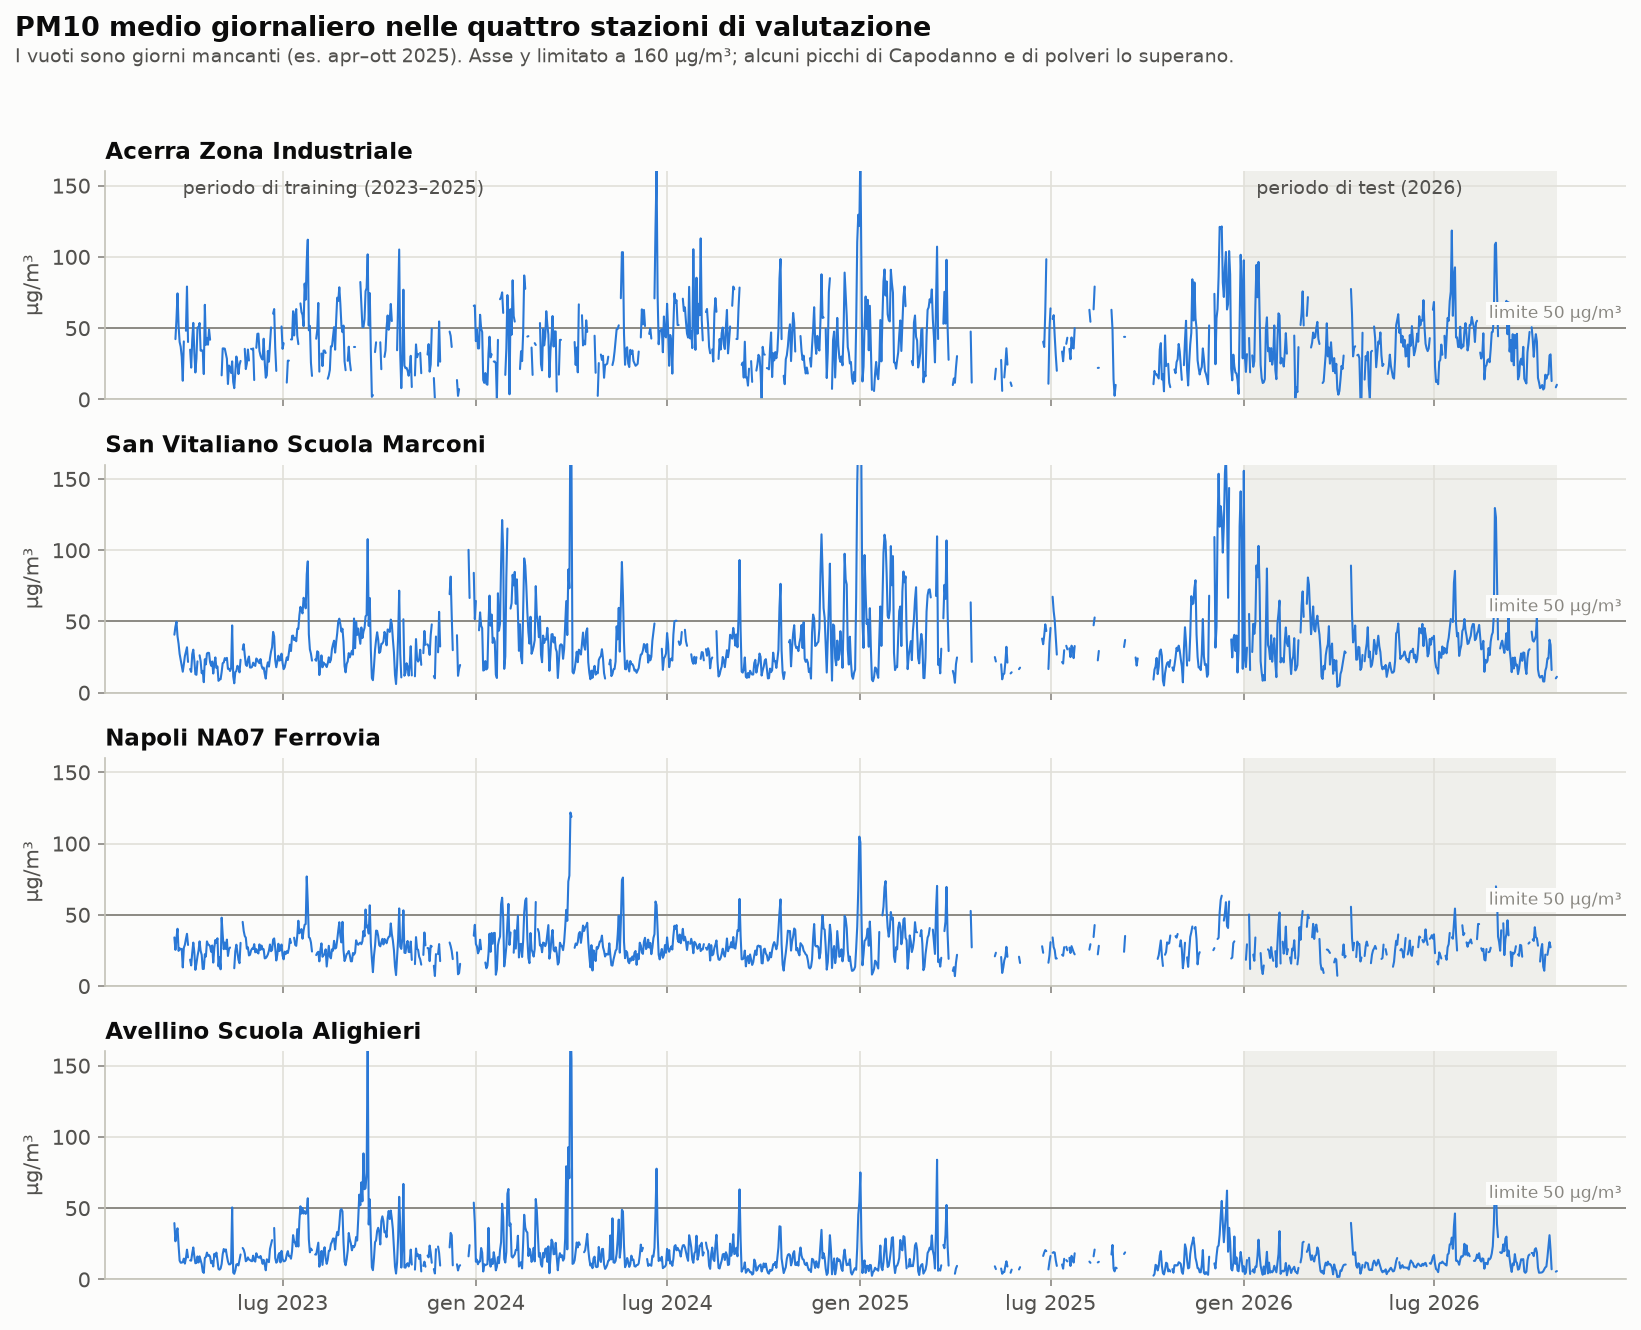
\includegraphics[width=0.9\textwidth]{01_data_train_test.png}
  \caption{PM10 giornaliero nelle quattro stazioni; il periodo di test 2026 è ombreggiato.}
  \label{fig:fc_serie}
\end{figure}

La Figura~\ref{fig:fc_serie} mostra le quattro serie. Sono evidenti le lacune già
descritte nella Sezione~\ref{sec:continuita}, in particolare tra aprile e ottobre
2025, oltre a singoli giorni mancanti. Le stazioni inquinate (Acerra e San
Vitaliano) superano spesso il limite di \SI{50}{\micro\gram\per\cubic\metre},
Avellino quasi mai.

% ------------------------------------------------------------
\section{Preparazione dei dati}
\label{sec:fc_preparazione}

La preparazione dei dati segue quattro passi.
\begin{enumerate}
  \item \textbf{Pulizia dei dati orari}, con le stesse regole del pre-processing
        (Sezione~\ref{sec:preprocessing}): si rimuovono il codice di valore
        mancante $-9999$, i valori negativi, i valori fisicamente impossibili, i
        sensori ``bloccati'' (lo stesso valore estremo per almeno 6 ore) e le serie
        stazione $\times$ inquinante $\times$ anno interamente nulle.
  \item \textbf{Media giornaliera}: un giorno è valido solo se almeno 18 delle sue
        24 ore sono valide, secondo la regola del 75\% del D.Lgs.\ 155/2010. I
        giorni con meno ore valide restano \emph{mancanti} e non vengono riempiti.
  \item \textbf{Massimo giornaliero della media mobile su 8 ore per
        l'O\textsubscript{3} (MDA8)}: per ogni ora si calcola la media delle 8 ore
        precedenti, valida se almeno 6 ore su 8 sono valide; il massimo del giorno è
        valido se almeno 18 delle 24 medie sono valide. È l'indicatore su cui è
        definito il valore obiettivo dell'O\textsubscript{3}
        (\SI{120}{\micro\gram\per\cubic\metre}).
  \item \textbf{Trasformazione logaritmica}: tutti i modelli lavorano su
        $\log(1+y)$ e la previsione viene riconvertita con $e^{x}-1$. Le
        concentrazioni sono fortemente asimmetriche a destra
        (Sezione~\ref{sec:statistiche}), mentre su scala logaritmica la
        distribuzione è approssimativamente simmetrica, come assumono ARIMA e
        Prophet; inoltre la previsione non può mai essere negativa. La
        trasformazione ha anche un costo, discusso nella
        Sezione~\ref{sec:fc_picchi}.
\end{enumerate}

Ogni modello gestisce i giorni mancanti in modo diverso
(Tabella~\ref{tab:fc_mancanti}).

\begin{table}[H]
  \centering
  \caption{Gestione dei giorni mancanti nei diversi modelli.}
  \label{tab:fc_mancanti}
  \small
  \begin{tabularx}{\textwidth}{@{}l X@{}}
    \toprule
    \textbf{Modello} & \textbf{Gestione dei giorni mancanti} \\
    \midrule
    ARIMA / SARIMAX & Nativa, tramite il filtro di Kalman: un giorno mancante è semplicemente ``non osservato'' e il modello continua a prevedere attraverso la lacuna \\
    \addlinespace
    Prophet & I giorni mancanti vengono scartati, poiché Prophet non richiede una serie regolare \\
    \addlinespace
    XGBoost & Le feature ritardate diventano mancanti; XGBoost apprende, a ogni divisione dell'albero, una direzione predefinita per i valori mancanti \\
    \bottomrule
  \end{tabularx}
\end{table}

% ------------------------------------------------------------
\section{Valutazione dei modelli}
\label{sec:fc_valutazione}

\subsection{Previsione a un passo con parametri fissi}
Ogni modello viene \textbf{stimato una sola volta} sul periodo di training. Per
ogni giorno di test $t$, il modello prevede $t$ utilizzando tutte le osservazioni
fino al giorno $t-1$. I parametri \textbf{non vengono ristimati} durante il test:
il modello si limita a incorporare le nuove osservazioni man mano che arrivano.

Questo schema simula un contesto operativo, in cui ogni sera si prevede il giorno
successivo, ed è equo: nessun modello vede mai il giorno che sta prevedendo.

\subsection{Campione comune}
Le metriche sono calcolate solo sui giorni-stazione in cui l'osservazione è valida
e tutti i modelli hanno prodotto una previsione, così che nessun modello sia
avvantaggiato dall'essere valutato su giorni ``più facili''. Per il PM10 si tratta
di \num{1038} giorni-stazione, di cui 105 sopra
\SI{50}{\micro\gram\per\cubic\metre}.

\subsection{Metriche}
Le metriche utilizzate sono riportate nella Tabella~\ref{tab:fc_metriche}.

\begin{table}[H]
  \centering
  \caption{Metriche di valutazione.}
  \label{tab:fc_metriche}
  \small
  \begin{tabularx}{\textwidth}{@{}>{\raggedright\arraybackslash}p{3cm} >{\raggedright\arraybackslash}X >{\raggedright\arraybackslash}X@{}}
    \toprule
    \textbf{Metrica} & \textbf{Cosa misura} & \textbf{Come leggerla} \\
    \midrule
    MAE (\emph{mean absolute error}) & Ampiezza media dell'errore, nell'unità dell'inquinante & Metrica principale: in media la previsione sbaglia di $X$ \ugm \\
    \addlinespace
    RMSE (\emph{root mean squared error}) & Come il MAE, ma gli errori grandi pesano di più & Un RMSE alto rispetto al MAE indica errori grandi occasionali \\
    \addlinespace
    Bias & Media di (previsto $-$ osservato) & Negativo: il modello prevede in media valori troppo bassi \\
    \addlinespace
    Skill vs persistenza & $1 - \mathrm{MAE}_{\text{modello}} / \mathrm{MAE}_{\text{persistenza}}$ & Quanto il modello è migliore di ``domani = oggi'': 0\% indica nessun miglioramento, un valore negativo un peggioramento. Non dipende dall'unità di misura ed è quindi l'unica metrica confrontabile tra inquinanti \\
    \addlinespace
    Precision (superamenti) & Tra i giorni previsti sopra la soglia, quota di quelli realmente sopra & Alta: pochi falsi allarmi \\
    \addlinespace
    Recall (superamenti) & Tra i giorni realmente sopra la soglia, quota di quelli previsti sopra & Alta: pochi episodi mancati \\
    \addlinespace
    F1 & Media armonica di precision e recall & Un unico numero che le riassume \\
    \bottomrule
  \end{tabularx}
\end{table}

Quando un modello non prevede mai un superamento, la precision non è calcolabile e
nelle tabelle compare ``--''. Non si utilizza il MAPE (errore percentuale medio),
perché gli errori percentuali esplodono nei giorni puliti, con valori vicini a
zero: la metrica sarebbe dominata proprio dai giorni meno importanti.

% ------------------------------------------------------------
\section{Baseline}
\label{sec:fc_baseline}

Un modello è utile solo se fa meglio di una previsione banale. Si utilizzano due
\emph{baseline}:
\begin{itemize}
  \item \textbf{persistenza}: domani = oggi (l'ultimo valore osservato). Per la
        qualità dell'aria è sorprendentemente difficile da battere, perché gli
        episodi di inquinamento durano diversi giorni;
  \item \textbf{seasonal naive} ($t-7$): domani = lo stesso giorno della settimana
        precedente. Verifica se il solo ciclo settimanale ha valore predittivo. Per
        il PM10 è molto peggiore della persistenza (MAE \num{13.9} contro
        \num{8.6}): \textbf{il ciclo settimanale è debole rispetto alla persistenza
        da un giorno all'altro}, in coerenza con quanto osservato nella
        Sezione~\ref{sec:temporale}.
\end{itemize}

% ------------------------------------------------------------
\section{ARIMA}
\label{sec:fc_arima}

\subsection{Il modello}
Un modello ARIMA($p$, $d$, $q$) spiega il valore di oggi con tre componenti:
\begin{itemize}
  \item \textbf{AR($p$), autoregressiva}: il valore di oggi dipende dai $p$ giorni
        precedenti,
        \[ y_t = c + \phi_1 y_{t-1} + \dots + \phi_p y_{t-p} + \varepsilon_t; \]
  \item \textbf{I($d$), integrata}: la serie viene differenziata $d$ volte
        ($y_t - y_{t-1}$) per rimuovere i trend; con $d=0$ la serie oscilla
        attorno a una media stabile;
  \item \textbf{MA($q$), media mobile}: il valore di oggi dipende anche dagli
        ultimi $q$ errori di previsione ($\theta_1\varepsilon_{t-1} + \dots +
        \theta_q\varepsilon_{t-q}$), il che permette al modello di correggersi
        quando ha sbagliato di recente.
\end{itemize}

\subsection{ACF e PACF}

\begin{figure}[H]
  \centering
  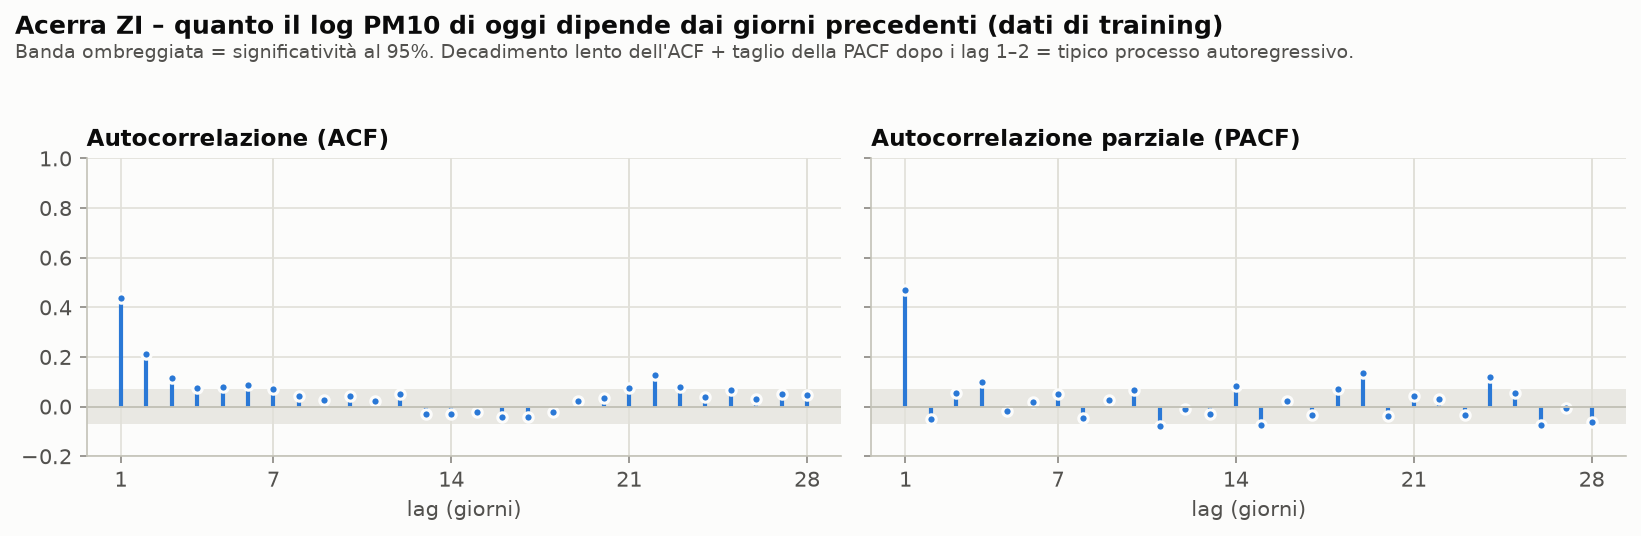
\includegraphics[width=0.9\textwidth]{02_acf_pacf_acerra.png}
  \caption{Autocorrelazione (sinistra) e autocorrelazione parziale (destra) del logaritmo del PM10 ad Acerra, dati di training.}
  \label{fig:fc_acf}
\end{figure}

La Figura~\ref{fig:fc_acf} riporta le funzioni di autocorrelazione del logaritmo
del PM10 ad Acerra.
\begin{itemize}
  \item L'\textbf{ACF} (correlazione tra oggi e $k$ giorni prima) vale \num{0.44}
        al ritardo 1 e \num{0.21} al ritardo 2, poi decade lentamente verso zero:
        ieri conta molto, l'altro ieri un po', e la memoria si esaurisce in circa
        una settimana.
  \item La \textbf{PACF} (correlazione al ritardo $k$ dopo aver rimosso l'effetto
        dei ritardi più brevi) presenta un unico picco forte al ritardo 1
        (\num{0.47}) e valori quasi nulli in seguito. È la firma di un
        \textbf{processo di tipo AR(1)}: la maggior parte dell'informazione del
        passato è contenuta nel valore di ieri.
  \item I picchi ai ritardi 7, 14 e 21 sono piccoli: il ciclo settimanale esiste ma
        è debole, coerentemente con lo scarso risultato della seasonal naive.
\end{itemize}

\subsection{Scelta dell'ordine}
Invece di leggere gli ordini dai grafici, lo script prova ogni combinazione
$p \in \{0,\dots,3\}$, $d \in \{0,1\}$, $q \in \{0,\dots,3\}$ (32 modelli per
stazione) e sceglie quella con l'\textbf{AIC} (\emph{Akaike Information
Criterion}) più basso, che premia la bontà di adattamento e penalizza la
complessità. Gli ordini selezionati per il PM10 sono riportati nella
Tabella~\ref{tab:fc_ordini_arima}.

\begin{table}[H]
  \centering
  \caption{Ordini ARIMA selezionati per il PM10.}
  \label{tab:fc_ordini_arima}
  \small
  \begin{tabular}{l l}
    \toprule
    \textbf{Stazione} & \textbf{ARIMA selezionato} \\
    \midrule
    Acerra ZI & ARIMA(1, 0, 3) \\
    San Vitaliano & ARIMA(2, 0, 2) \\
    Napoli Ferrovia & ARIMA(1, 0, 1) \\
    Avellino & ARIMA(1, 1, 3) \\
    \bottomrule
  \end{tabular}
\end{table}

Il valore $d=0$ in tre stazioni su quattro conferma che, in questo periodo, il PM10
non presenta un trend che richieda una differenziazione, ma oscilla attorno a un
livello stabile.

\subsection{Limiti}
ARIMA conosce solo il passato recente della serie stessa: non ha alcuna nozione di
stagione, giorno della settimana, festività o meteo. In inverno ``impara'' che
l'inquinamento è alto solo dopo aver osservato alcuni giorni con valori alti.

% ------------------------------------------------------------
\section{SARIMAX}
\label{sec:fc_sarimax}

SARIMAX (\emph{Seasonal ARIMA with eXogenous variables}) aggiunge due elementi al
modello ARIMA.

\subsection{Componente stagionale}
La componente stagionale ($P$, $D$, $Q$, $s$) applica la stessa logica
(autoregressione, differenziazione, media mobile) al ritardo $s$ invece che al
ritardo 1. Con $s=7$ il valore di oggi può dipendere anche dallo stesso giorno della
settimana precedente. Lo script confronta 12 combinazioni (4 ordini non stagionali
$\times$ 3 stagionali) e sceglie quella con l'AIC più basso. Per il PM10, in tre
stazioni è stato selezionato il modello
\textbf{SARIMAX(1,0,1)$\times$(1,0,1,7)}, con un termine AR e uno MA al ritardo 1
e un termine AR e uno MA al ritardo 7. Ad Avellino è stato scelto
\textbf{SARIMAX(2,1,2)$\times$(1,0,1,7)}, con una differenziazione, coerente con
l'ARIMA(1,1,3) della stessa stazione.

\subsection{Regressori esogeni}
I regressori esogeni sono variabili esterne note in anticipo, che entrano
nell'equazione come in una regressione lineare:
\begin{itemize}
  \item \textbf{termini di Fourier per il ciclo annuale},
        $\sin(2\pi k t / 365{,}25)$ e $\cos(2\pi k t / 365{,}25)$ per $k=1,2$:
        quattro onde regolari che permettono al modello di rappresentare
        l'andamento inverno/estate;
  \item \textbf{indicatore di festività}: festività nazionali italiane e 31
        dicembre (fuochi d'artificio, Sezione~\ref{sec:eventi}).
\end{itemize}

Si utilizzano i termini di Fourier invece di una stagione $s=365$ perché un ARIMA
stagionale annuale richiederebbe centinaia di stati ritardati: sarebbe
estremamente lento e instabile e, con circa \num{2.8} anni di training, vedrebbe
meno di tre cicli. I termini di Fourier descrivono la forma annuale con soli 4
parametri.

\subsection{Risultato}
Per il PM10 SARIMAX migliora ARIMA solo marginalmente (MAE \num{7.97} contro
\num{8.02}). A un giorno di distanza il valore di ieri contiene già l'informazione
stagionale (``è inverno, quindi ieri era alto, quindi oggi sarà alto''). Ci si
aspetterebbe che la componente stagionale diventi più utile a orizzonti più lunghi,
dove il passato recente è meno informativo; la Sezione~\ref{sec:fc_errore_h} mostra
che anche a sette giorni il vantaggio su ARIMA resta piccolo.

% ------------------------------------------------------------
\section{Prophet}
\label{sec:fc_prophet}

\subsection{Il modello}
Prophet, sviluppato da Meta, non è un modello autoregressivo, ma un modello di
\emph{curve fitting} che scompone la serie in componenti additive:
\[ y(t) = \text{trend}(t) + \text{annuale}(t) + \text{settimanale}(t) + \text{festività}(t) + \varepsilon_t \]
dove:
\begin{itemize}
  \item il \textbf{trend} è una spezzata lineare che può cambiare pendenza in punti
        individuati automaticamente;
  \item le componenti \textbf{annuale} e \textbf{settimanale} sono curve
        periodiche regolari (serie di Fourier);
  \item le \textbf{festività} hanno ciascuna un effetto separato (qui, secondo il
        calendario italiano).
\end{itemize}
Poiché si modella il logaritmo della concentrazione, gli effetti additivi
diventano \textbf{moltiplicativi} sulla concentrazione: $+0{,}2$ su scala
logaritmica corrisponde a circa il 22\% in più.

\begin{figure}[H]
  \centering
  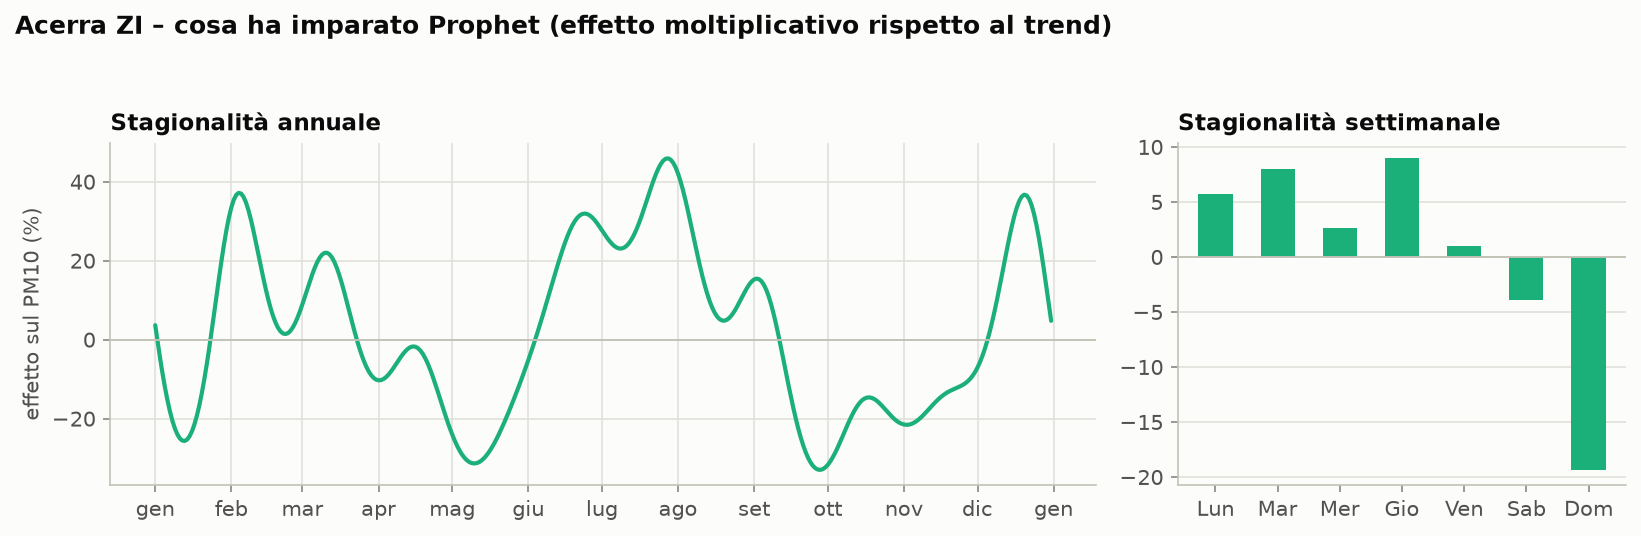
\includegraphics[width=0.9\textwidth]{03_prophet_components_acerra.png}
  \caption{Componenti stimate da Prophet ad Acerra, espresse come effetto percentuale sul PM10 rispetto al trend.}
  \label{fig:fc_prophet_comp}
\end{figure}

La Figura~\ref{fig:fc_prophet_comp} mostra le componenti apprese ad Acerra.
\begin{itemize}
  \item \textbf{Settimanale}: la domenica è circa il 19\% più bassa e il sabato
        circa il 4\% più basso, mentre i giorni feriali sono dall'1 al 9\% più
        alti. È il segnale del traffico già osservato nella
        Sezione~\ref{sec:temporale}.
  \item \textbf{Annuale}: la curva è \textbf{molto ondulata}, con massimi a
        febbraio, tra fine luglio e agosto ($+45$\%) e a metà dicembre, e minimi a
        maggio e ottobre (circa $-30$\%). In parte l'andamento è reale
        (riscaldamento invernale, polveri estive), ma in buona parte è
        \textbf{overfitting}: con meno di tre anni di dati, la curva annuale
        flessibile di Prophet memorizza episodi specifici, come le polveri e gli
        incendi dell'estate 2024, come se si ripetessero ogni anno.
  \item \textbf{Festività}: Prophet ha appreso un forte effetto di Capodanno dai
        fuochi d'artificio presenti nei dati di training
        (Sezione~\ref{sec:eventi}); per questo prevede circa
        \SI{150}{\micro\gram\per\cubic\metre} a San Vitaliano il 1° gennaio 2026
        (Figura~\ref{fig:fc_test}).
\end{itemize}

\subsection{Limiti di Prophet}
La previsione di Prophet per una certa data \textbf{dipende solo dal calendario},
non da ciò che è accaduto il giorno prima. Se inizia un episodio di inquinamento,
Prophet non può accorgersene e continua a prevedere la media stagionale. Per questo,
sul PM10, Prophet è \textbf{peggiore della persistenza del 21\%}: perde tutta la
dinamica da un giorno all'altro, che contiene la maggior parte della
prevedibilità. Per gli altri inquinanti il risultato è ancora peggiore
(Sezione~\ref{sec:fc_altri_skill}).

\subsection{Prophet con valori ritardati}
Prophet permette di aggiungere \textbf{regressori} esterni. Aggiungendo l'ultimo
valore osservato e la media degli ultimi 7 giorni, entrambi noti la sera del giorno
$t-1$, diventa un modello quasi autoregressivo (nel seguito \emph{Prophet + lag}).
Con questi regressori Prophet diventa competitivo sul PM10 (MAE \num{8.01} e il
miglior RMSE, \num{13.04}), comportandosi di fatto come una regressione lineare sui
valori recenti con una stagionalità regolare.

Prophet descrive quindi bene stagionalità e festività, ma da solo non è uno
strumento adatto alla previsione a breve termine di una serie dominata dalla
persistenza.

% ------------------------------------------------------------
\section{XGBoost}
\label{sec:fc_xgboost}

\subsection{Il modello}
XGBoost non è un modello per serie temporali, ma un modello di \emph{gradient
boosting} su alberi decisionali per la regressione. Per utilizzarlo nel
forecasting, il problema viene trasformato in una tabella con \textbf{una riga per
giorno-stazione}, che contiene il target (il logaritmo della concentrazione del
giorno) e \textbf{feature costruite solo con le informazioni disponibili la sera
precedente}.

Il boosting costruisce gli alberi in sequenza: ogni nuovo albero corregge gli
errori della somma dei precedenti. Gli alberi possono rappresentare \textbf{effetti
non lineari e interazioni} (ad esempio ``ieri il valore era alto, siamo in inverno
e la media regionale sta salendo''), che ARIMA non può cogliere.

\subsection{Feature utilizzate}
Le feature sono riportate nella Tabella~\ref{tab:fc_feature}.

\begin{table}[H]
  \centering
  \caption{Feature utilizzate dal modello XGBoost.}
  \label{tab:fc_feature}
  \small
  \begin{tabularx}{\textwidth}{@{}>{\raggedright\arraybackslash}p{4cm} >{\raggedright\arraybackslash}X@{}}
    \toprule
    \textbf{Gruppo} & \textbf{Feature} \\
    \midrule
    Valori recenti del target nella stazione & Valori di 1, 2, 3, 7 e 14 giorni prima; ultimo valore osservato (riportato in avanti sui giorni mancanti); medie a 7 e 30 giorni \\
    \addlinespace
    Altri inquinanti del giorno precedente & PM10, PM2,5, NO\textsubscript{2} e O\textsubscript{3} della stessa stazione, escluso il target \\
    \addlinespace
    Segnale regionale & Media del target su tutte le stazioni 1 e 2 giorni prima, per cogliere episodi a scala regionale come le polveri sahariane \\
    \addlinespace
    Calendario & Giorno della settimana, giorno dell'anno (seno e coseno), mese, indicatore di festività \\
    \addlinespace
    Stazione & Codice della stazione (categorico), così che un unico modello possa apprendere livelli specifici per stazione \\
    \bottomrule
  \end{tabularx}
\end{table}

\subsection{Un modello globale per inquinante}
Invece di un modello per stazione, per ogni inquinante XGBoost viene addestrato
\textbf{una sola volta su tutte le stazioni fisse che lo misurano}. Per il PM10 si
tratta di 35 stazioni, cioè circa \num{26500} righe di training invece di circa
800. Il modello può così apprendere comportamenti generali (ad esempio come evolve
il PM10 dopo un giorno con valori alti) dall'intera rete, e poi specializzarsi per
stazione.

\subsection{Controllo dell'overfitting}
Gli ultimi 90 giorni del periodo di training vengono tenuti da parte per
determinare il numero di alberi (\emph{early stopping}). Per il PM10 il training si
è fermato a 108 alberi; il modello finale viene poi ristimato sull'intero periodo
di training con questo numero di alberi.

\subsection{Importanza delle feature}

\begin{figure}[H]
  \centering
  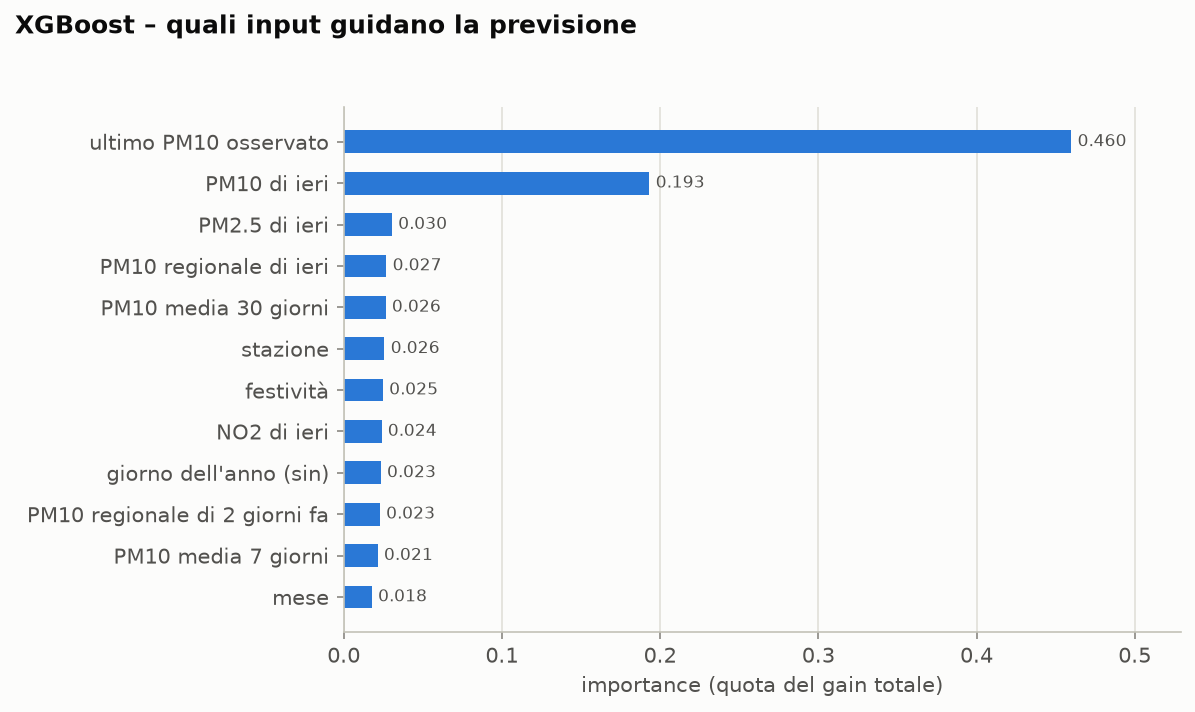
\includegraphics[width=0.9\textwidth]{10_xgboost_feature_importance.png}
  \caption{Quota del \emph{gain} totale (riduzione dell'errore) apportata da ciascuna feature nel modello XGBoost per il PM10.}
  \label{fig:fc_xgb_imp}
\end{figure}

Come mostra la Figura~\ref{fig:fc_xgb_imp}, circa il \textbf{65\%} del potere
predittivo proviene da due feature: l'\textbf{ultimo PM10 osservato} e il
\textbf{PM10 del giorno precedente} (esistono entrambe perché il valore di ieri a
volte manca, e in quel caso l'informazione è portata dall'ultimo valore osservato).
Le altre feature contribuiscono per il 2--3\% ciascuna: PM2,5 del giorno
precedente, PM10 regionale, livello a 30 giorni, stazione, festività,
NO\textsubscript{2} del giorno precedente e posizione stagionale.

Il risultato conferma quanto indicato dall'ACF: \textbf{con i soli dati storici di
qualità dell'aria, la previsione è essenzialmente ``il valore di ieri, corretto''}.
La Sezione~\ref{sec:fc_altri_importanza} mostra che ciò vale per tutti gli
inquinanti.

% ------------------------------------------------------------
\section{Risultati per il PM10}
\label{sec:fc_risultati}

\subsection{Risultati complessivi}
La Tabella~\ref{tab:fc_risultati_pm10} riporta le metriche sulle quattro stazioni
aggregate (\num{1038} giorni di test).

\begin{table}[H]
  \centering
  \caption{Risultati della previsione a un giorno per il PM10 (4 stazioni, \num{1038} giorni-stazione). MAE, RMSE e bias in \ugm; precision, recall e F1 riferite ai giorni con PM10 $> 50$ \ugm.}
  \label{tab:fc_risultati_pm10}
  \small
  \begin{tabular}{l r r r r r r r}
    \toprule
    \textbf{Modello} & \textbf{MAE} & \textbf{RMSE} & \textbf{Bias} & \textbf{Prec.} & \textbf{Recall} & \textbf{F1} & \textbf{Skill} \\
    \midrule
    XGBoost & \textbf{7,91} & 13,25 & $-2{,}22$ & \textbf{0,72} & 0,22 & 0,34 & $\mathbf{+7{,}7}$\% \\
    SARIMAX & 7,97 & 13,61 & $-1{,}47$ & 0,71 & 0,29 & 0,41 & $+7{,}0$\% \\
    Prophet + lag & 8,01 & \textbf{13,04} & $-2{,}14$ & 0,62 & 0,25 & 0,35 & $+6{,}5$\% \\
    ARIMA & 8,02 & 13,73 & $-1{,}70$ & 0,65 & 0,23 & 0,34 & $+6{,}4$\% \\
    Persistenza & 8,57 & 15,01 & $+0{,}04$ & 0,55 & \textbf{0,55} & \textbf{0,55} & 0\% \\
    Prophet & 10,37 & 15,43 & $-1{,}92$ & 0,25 & 0,06 & 0,09 & $-21{,}1$\% \\
    Seasonal naive ($t-7$) & 13,93 & 20,98 & $+0{,}41$ & 0,24 & 0,25 & 0,24 & $-62{,}6$\% \\
    \bottomrule
  \end{tabular}
\end{table}

I quattro modelli principali ottengono un MAE quasi identico, circa
\SI{8}{\micro\gram\per\cubic\metre}, e battono la persistenza solo del 6--8\%. La
persistenza ha il MAE peggiore tra questi modelli, ma l'\textbf{F1 migliore} sui
superamenti (\num{0.55} contro \num{0.34}--\num{0.41}); il motivo è spiegato nella
Sezione~\ref{sec:fc_picchi}.

\subsection{Previsioni sul periodo di test}

\begin{figure}[H]
  \centering
  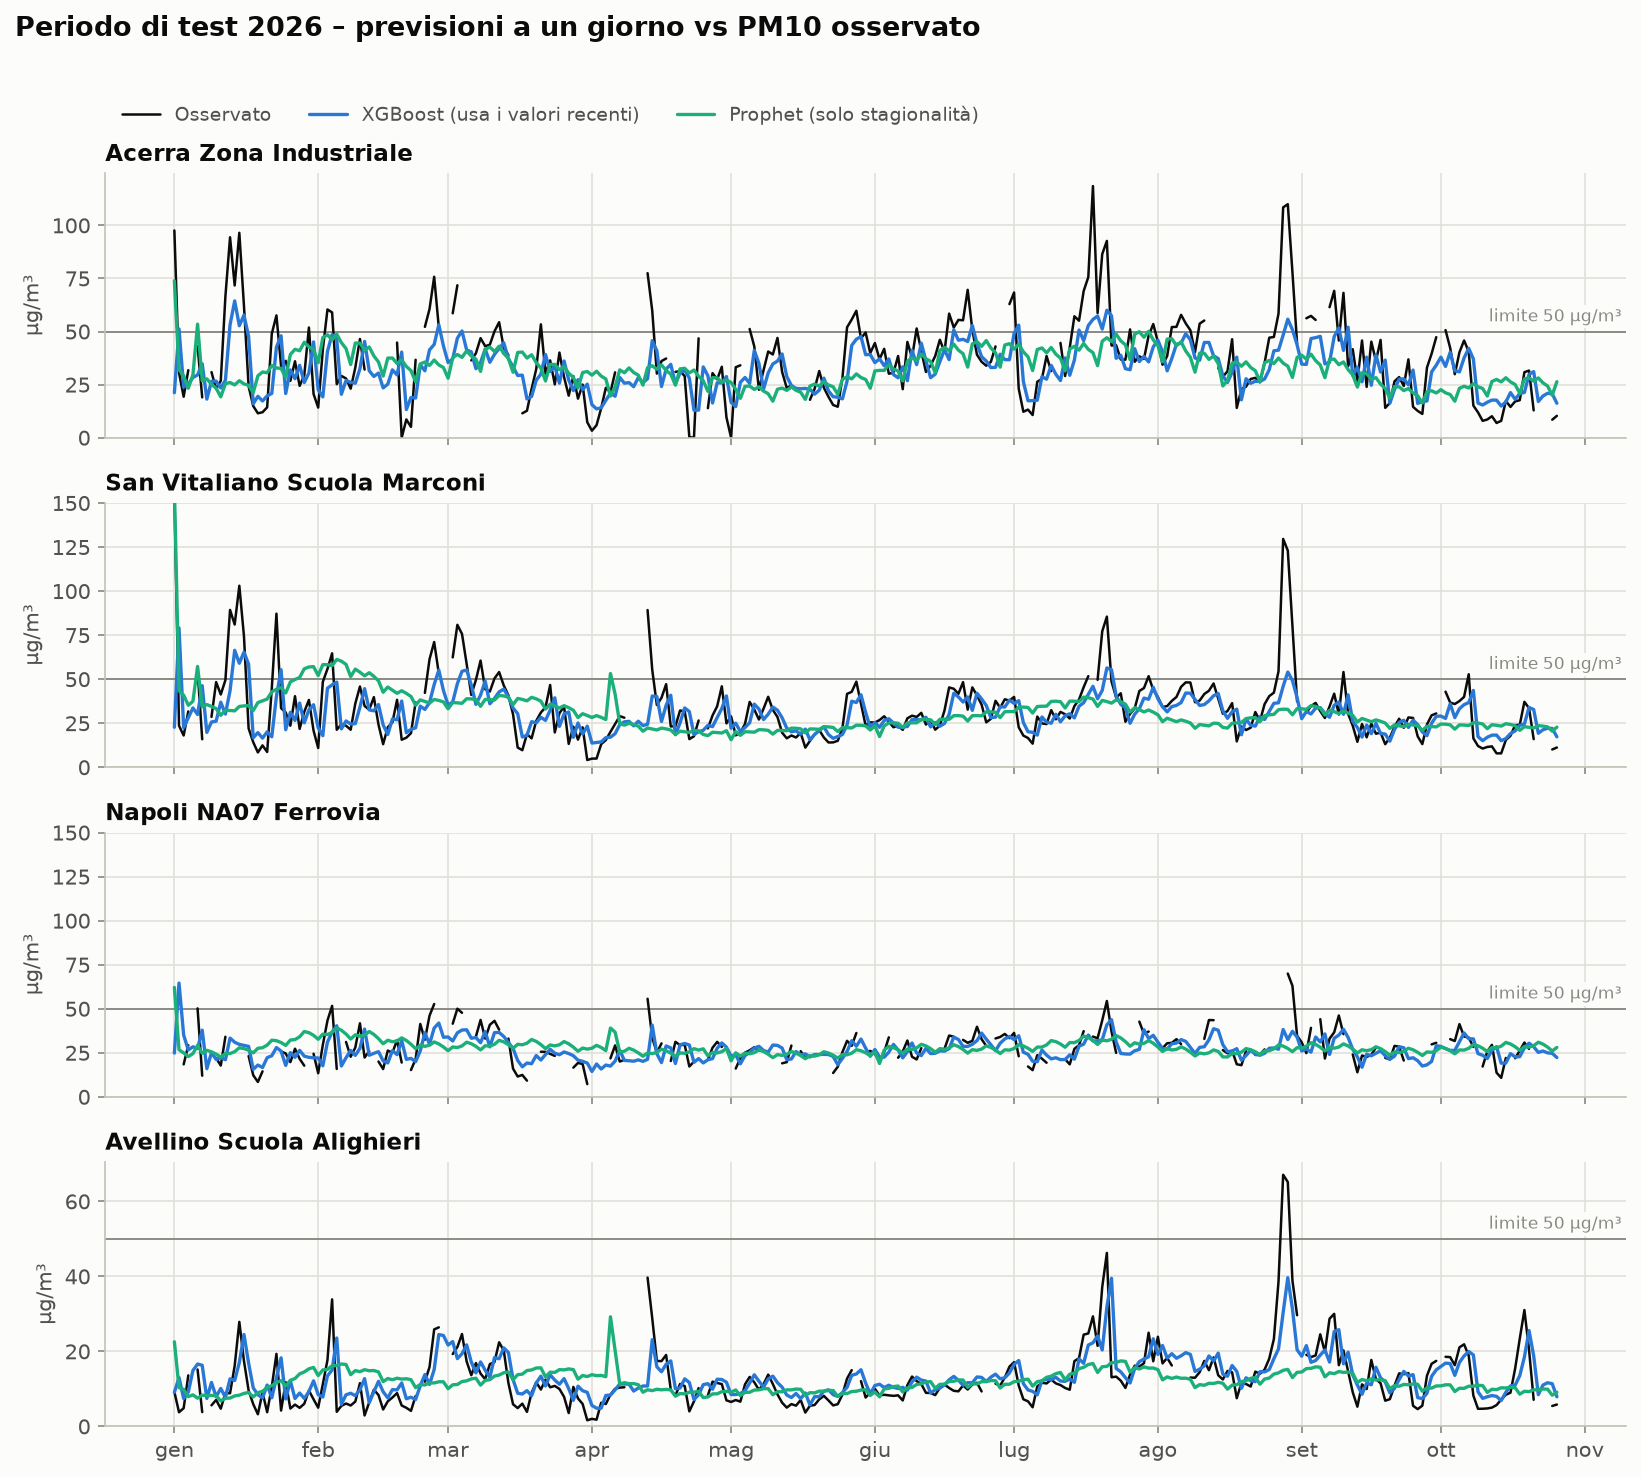
\includegraphics[width=0.9\textwidth]{04_forecast_test_period.png}
  \caption{PM10 osservato (nero), previsione XGBoost (blu) e Prophet standard (verde) sul periodo di test 2026.}
  \label{fig:fc_test}
\end{figure}

Dalla Figura~\ref{fig:fc_test} emerge che:
\begin{itemize}
  \item \textbf{XGBoost segue le variazioni da un giorno all'altro}, perché è
        guidato dal valore del giorno precedente, e riproduce bene il livello
        generale in tutte le stazioni;
  \item \textbf{Prophet produce una curva stagionale regolare}: coglie il livello
        generale, ma non reagisce agli episodi (ad esempio ad Acerra e San
        Vitaliano a fine agosto) e presenta l'anomalo picco di Capodanno il 1°
        gennaio;
  \item \textbf{i picchi più alti sono sottostimati da entrambi i modelli} (fine
        luglio e fine agosto ad Acerra e San Vitaliano, fine agosto ad Avellino),
        come discusso nella Sezione~\ref{sec:fc_picchi}.
\end{itemize}

\subsection{Dettaglio: Acerra, gennaio--marzo 2026}

\begin{figure}[H]
  \centering
  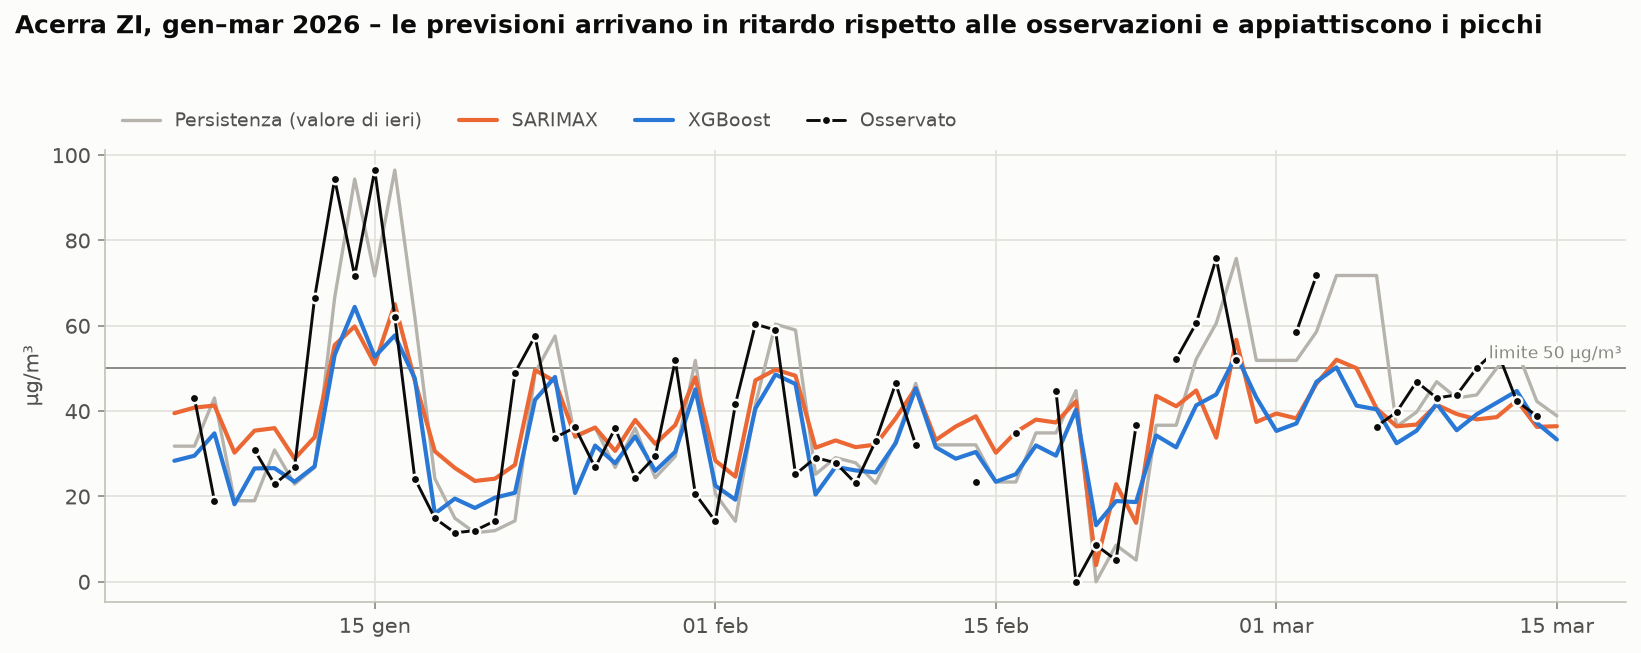
\includegraphics[width=0.9\textwidth]{05_zoom_acerra.png}
  \caption{PM10 ad Acerra, gennaio--marzo 2026: valori osservati (punti neri) e previsioni di persistenza (grigio), SARIMAX (arancione) e XGBoost (blu).}
  \label{fig:fc_zoom}
\end{figure}

La Figura~\ref{fig:fc_zoom} mostra il comportamento tipico di una previsione a un
giorno basata sui valori passati:
\begin{itemize}
  \item \textbf{le previsioni sono in ritardo di un giorno}: quando il PM10 passa da
        25 a \SI{95}{\micro\gram\per\cubic\metre} (metà gennaio), i modelli salgono
        solo il giorno \emph{successivo}, perché non hanno modo di sapere che il
        salto sta per arrivare;
  \item \textbf{i modelli riavvicinano la previsione della persistenza alla
        media}: dopo un giorno con valori alti la persistenza ripete il valore
        alto, mentre SARIMAX e XGBoost prevedono un valore intermedio. Questo
        riduce l'errore medio, perché molti giorni con valori alti sono seguiti da
        giorni con valori più bassi, ma fa sì che i modelli prevedano raramente
        valori sopra \SI{50}{\micro\gram\per\cubic\metre}.
\end{itemize}

\subsection{Risultati per stazione}

\begin{figure}[H]
  \centering
  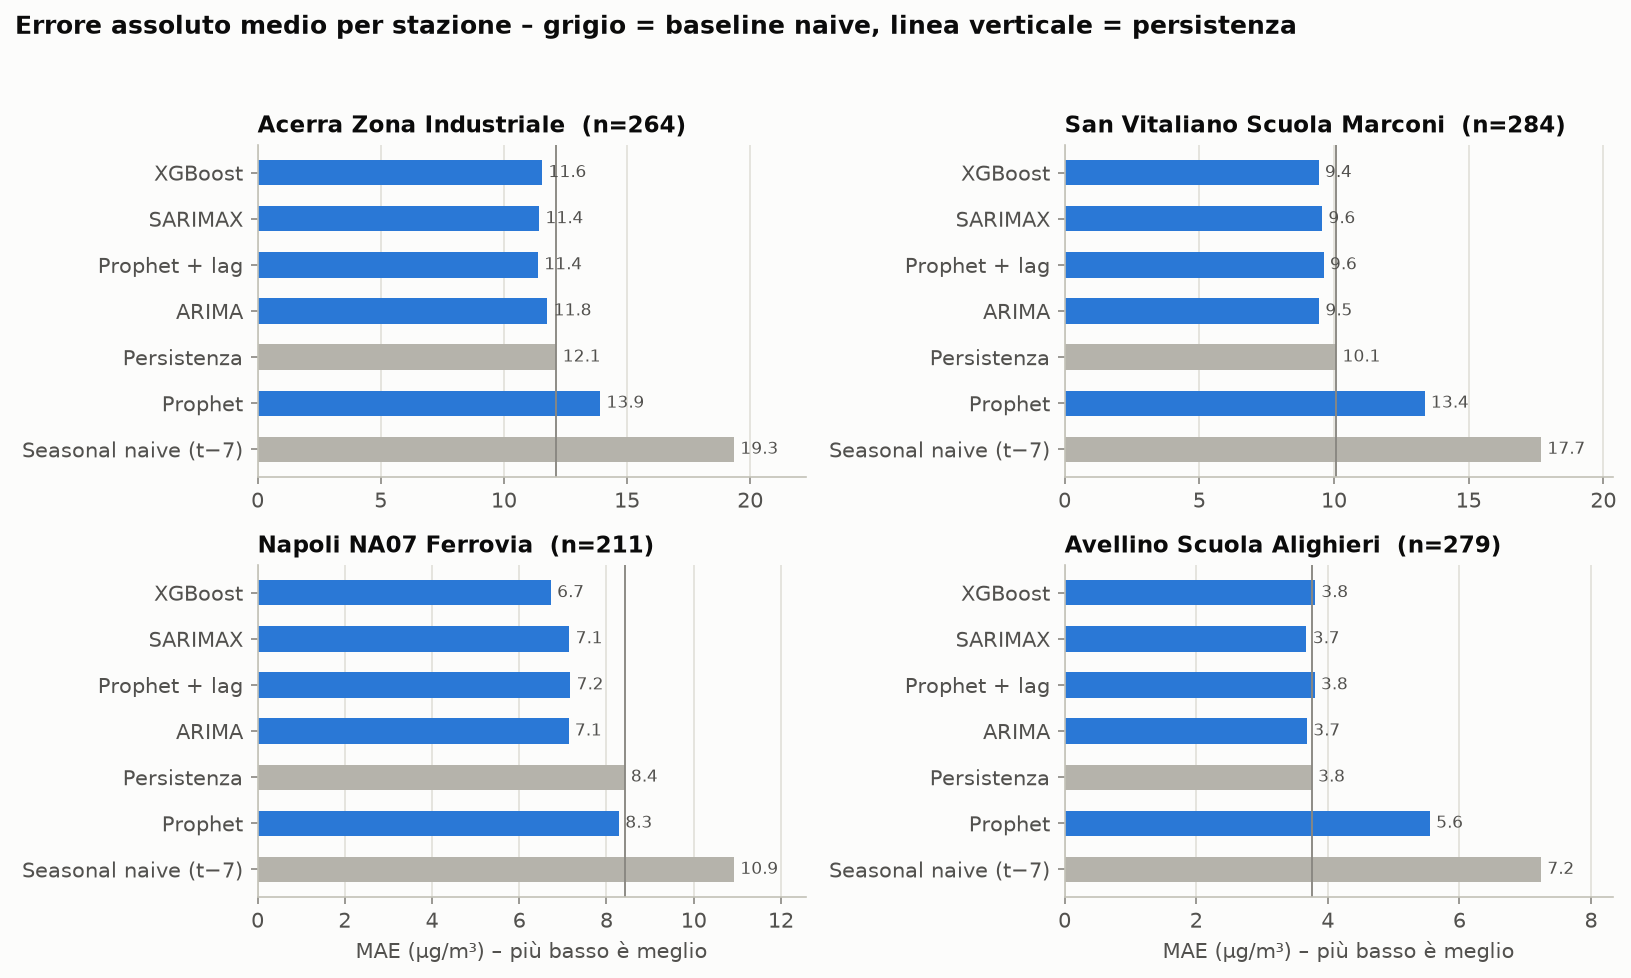
\includegraphics[width=0.9\textwidth]{06_mae_by_station.png}
  \caption{MAE per modello e stazione. Le barre grigie sono le baseline; la linea verticale indica la persistenza.}
  \label{fig:fc_mae_stazione}
\end{figure}

\begin{table}[H]
  \centering
  \caption{Risultati per stazione, PM10 (MAE in \ugm). Recall mod.: miglior recall tra i modelli ($^{a}$Prophet, gli altri modelli 0; $^{b}$SARIMAX e XGBoost; $^{c}$SARIMAX).}
  \label{tab:fc_stazioni_pm10}
  \footnotesize
  \setlength{\tabcolsep}{4pt}
  \begin{tabular}{l r r r l r r r}
    \toprule
    \textbf{Stazione} & \textbf{Giorni} & \textbf{$>50$} & \textbf{MAE pers.} & \textbf{Miglior modello} & \textbf{Skill} & \textbf{Recall pers.} & \textbf{Recall mod.} \\
    \midrule
    Napoli Ferrovia & 211 & 10 & 8,42 & XGBoost (6,73) & $+20{,}1$\% & 0,20 & 0,10$^{a}$ \\
    Acerra ZI & 264 & 62 & 12,13 & Prophet + lag (11,38) & $+6{,}2$\% & 0,63 & 0,24$^{b}$ \\
    San Vitaliano & 284 & 31 & 10,08 & XGBoost (9,43) & $+6{,}4$\% & 0,52 & 0,48$^{c}$ \\
    Avellino & 279 & 2 & 3,76 & SARIMAX (3,68) & $+2{,}1$\% & 0,50 & 0 \\
    \bottomrule
  \end{tabular}
\end{table}

Dalla Figura~\ref{fig:fc_mae_stazione} e dalla
Tabella~\ref{tab:fc_stazioni_pm10} emerge che:
\begin{itemize}
  \item gli errori crescono con il livello di inquinamento: il MAE è di circa
        11--\SI{12}{\micro\gram\per\cubic\metre} ad Acerra e di circa \num{3.7}
        ad Avellino;
  \item a \textbf{Napoli Ferrovia} XGBoost batte la persistenza del 20\%, il
        risultato migliore tra le quattro stazioni; tuttavia ARIMA, SARIMAX,
        XGBoost e Prophet + lag \textbf{non intercettano nessuno} dei 10
        superamenti;
  \item a \textbf{San Vitaliano} SARIMAX è l'unico caso in cui un modello batte la
        persistenza anche sui superamenti (F1 \num{0.57} contro \num{0.52});
  \item ad \textbf{Avellino}, sito pulito, nessun modello batte la persistenza in
        modo significativo, perché c'è poco segnale da un giorno all'altro da
        sfruttare; con soli 2 superamenti, precision e recall non sono
        significative;
  \item la \textbf{classifica tra ARIMA, SARIMAX, XGBoost e Prophet + lag cambia da
        stazione a stazione}: le loro differenze, di pochi decimi di \ugm,
        rientrano nella variabilità di un test di 10 mesi, e i quattro modelli
        vanno considerati \textbf{equivalenti}.
\end{itemize}

% ------------------------------------------------------------
\section{Perché i modelli sbagliano i giorni più inquinati}
\label{sec:fc_picchi}

È il risultato più importante per l'uso pratico della previsione. Vale per il PM10
e, come mostra la Sezione~\ref{sec:fc_altri_superamenti}, anche per gli altri
inquinanti con superamenti.

\subsection{Le evidenze}

\begin{figure}[H]
  \centering
  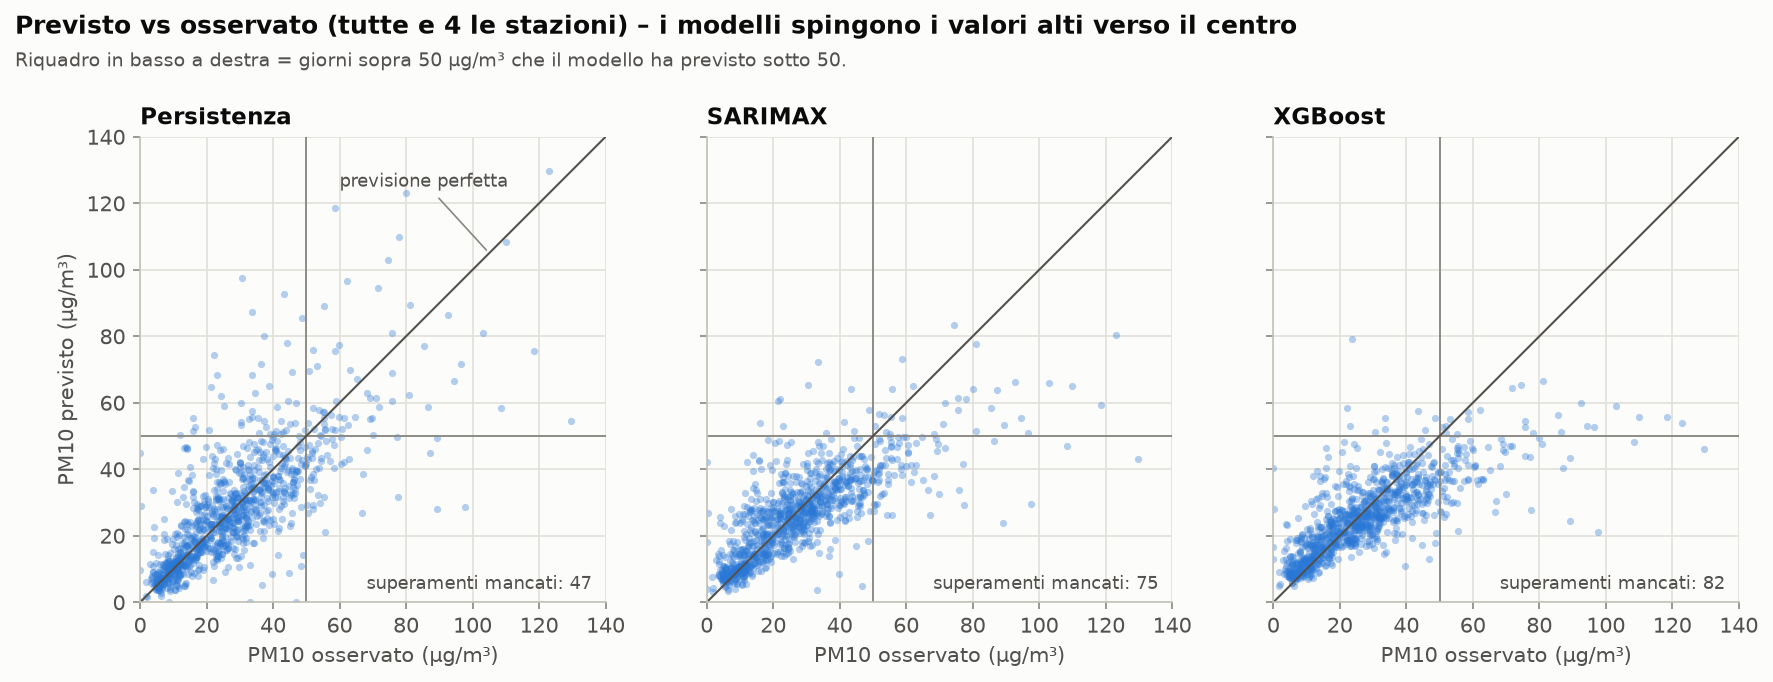
\includegraphics[width=0.9\textwidth]{07_scatter_forecast_vs_observed.png}
  \caption{Previsto contro osservato: ogni punto è un giorno-stazione e i punti sulla diagonale sono previsioni perfette. Il riquadro in basso a destra contiene i giorni sopra \SI{50}{\micro\gram\per\cubic\metre} previsti sotto tale soglia.}
  \label{fig:fc_scatter}
\end{figure}

Dei 105 giorni sopra \SI{50}{\micro\gram\per\cubic\metre} del periodo di test, la
persistenza ne manca 47, SARIMAX 75 e XGBoost 82. Le nuvole di punti dei modelli
nella Figura~\ref{fig:fc_scatter} sono visibilmente \textbf{più piatte della
diagonale}: ai valori osservati alti corrispondono previsioni tra 40 e
\SI{60}{\micro\gram\per\cubic\metre}.

\begin{figure}[H]
  \centering
  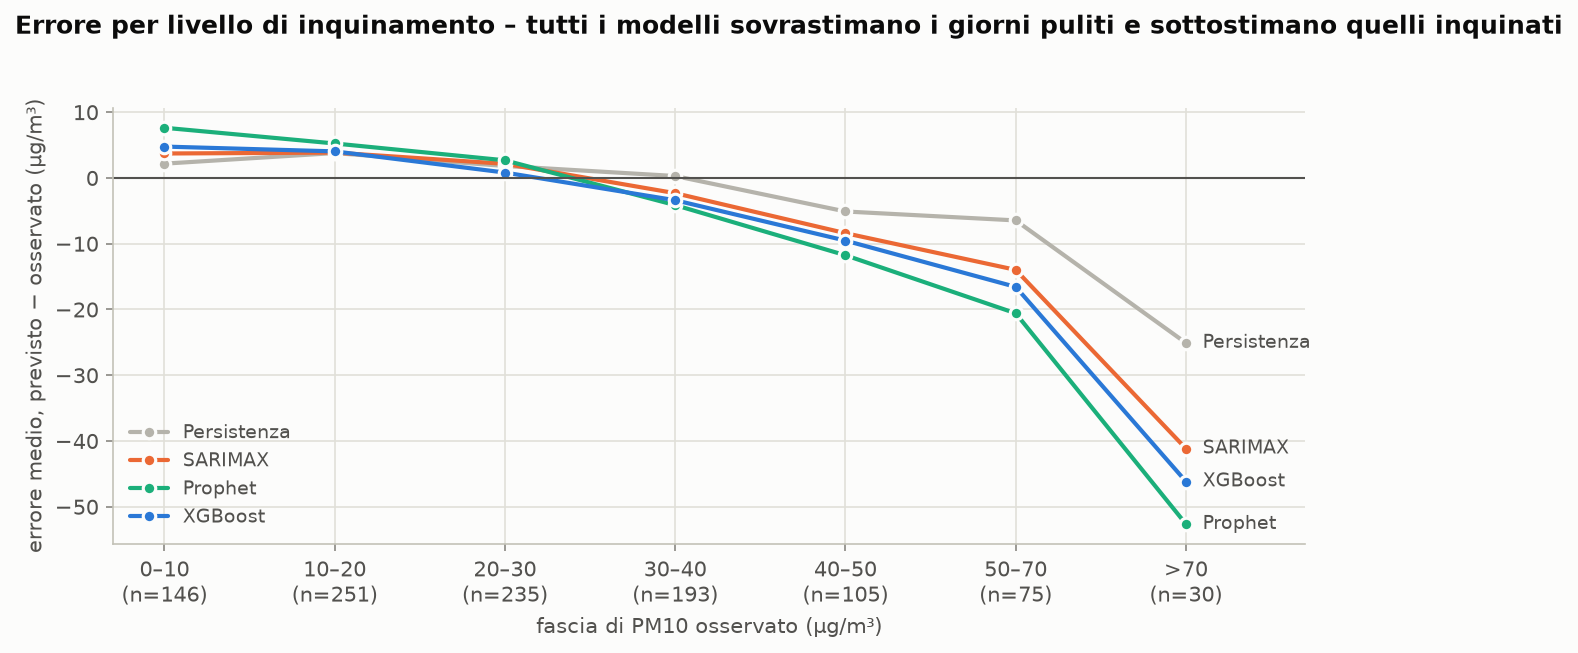
\includegraphics[width=0.9\textwidth]{08_bias_by_level.png}
  \caption{Errore medio per classe di PM10 osservato.}
  \label{fig:fc_bias_livello}
\end{figure}

La Figura~\ref{fig:fc_bias_livello} mostra che nei giorni puliti
(0--\SI{20}{\micro\gram\per\cubic\metre}) tutti i modelli prevedono valori
\textbf{troppo alti} (da $+2$ a $+7$~\ugm), mentre nei giorni sopra
\SI{70}{\micro\gram\per\cubic\metre} prevedono valori \textbf{molto più bassi}
dell'osservato: di circa 25~\ugm\ la persistenza, 41 SARIMAX, 46 XGBoost e 52
Prophet.

\begin{figure}[H]
  \centering
  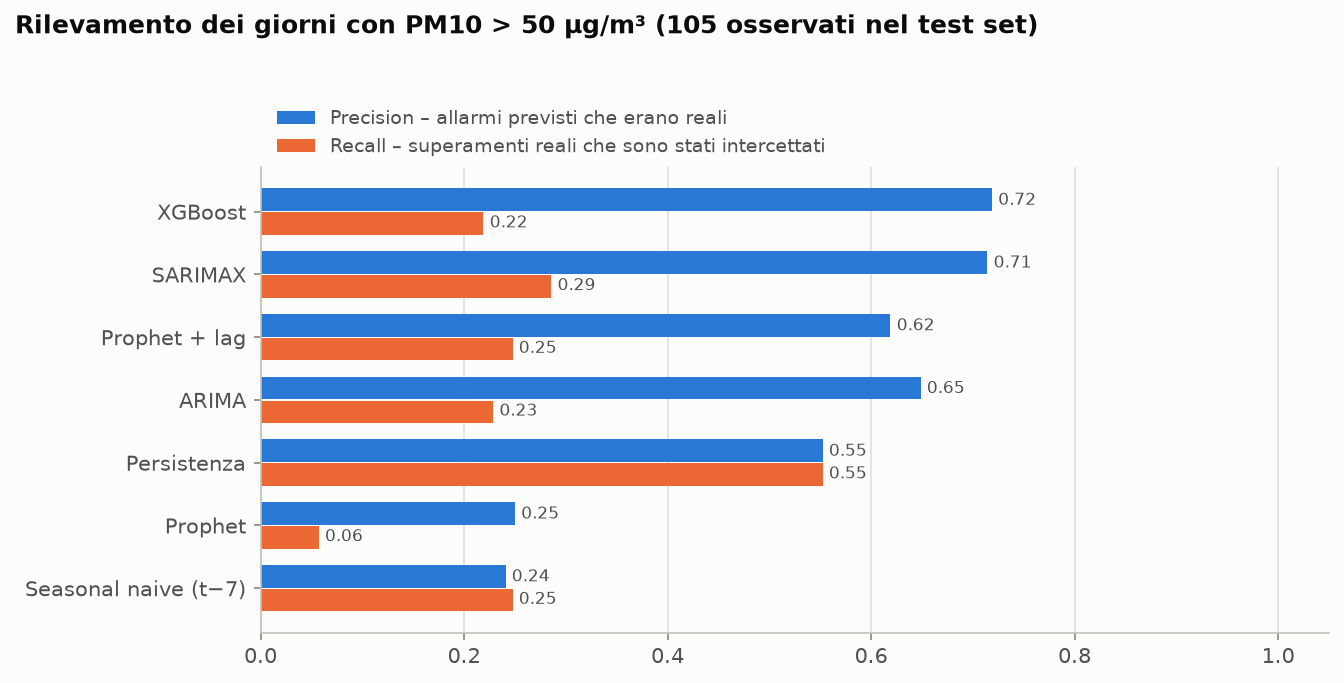
\includegraphics[width=0.9\textwidth]{09_exceedance_precision_recall.png}
  \caption{Precision e recall sui giorni con PM10 sopra \SI{50}{\micro\gram\per\cubic\metre}.}
  \label{fig:fc_prec_rec}
\end{figure}

Come mostra la Figura~\ref{fig:fc_prec_rec}, i modelli hanno una \textbf{precision
più alta} (quando prevedono un superamento, di solito è reale: 62--72\%), ma una
\textbf{recall molto più bassa}: intercettano solo il 22--29\% dei superamenti
reali, contro il 55\% della persistenza.

\subsection{Le cause}
\begin{enumerate}
  \item \textbf{Le previsioni che minimizzano l'errore vengono attirate verso la
        media} (\emph{regression to the mean}). I modelli sono addestrati a
        minimizzare l'errore quadratico e, quando il futuro è incerto, la stima
        che lo minimizza è il valore \emph{atteso}. Dopo un giorno con valori alti
        il PM10 a volte resta alto e a volte scende, quindi il valore atteso è
        inferiore a quello di oggi. Il modello si ``copre'' correttamente, ed è
        proprio questa prudenza a ridurre la recall sui superamenti. La
        persistenza non si copre: per questo ha il MAE peggiore ma la recall
        migliore.
  \item \textbf{La riconversione dalla scala logaritmica restituisce la mediana,
        non la media.} Se la previsione su scala logaritmica è $m$ con incertezza
        $\sigma$, allora $e^{m}$ è la previsione \emph{mediana} del PM10, mentre
        la \emph{media} è $e^{m+\sigma^2/2}$, più alta. Poiché il PM10 è
        asimmetrico a destra, ne deriva un errore sistematico verso il basso che
        cresce con il livello: è il bias negativo della
        Tabella~\ref{tab:fc_risultati_pm10}.
  \item \textbf{Manca l'informazione decisiva.} Gli episodi di inquinamento
        iniziano per cause \textbf{meteorologiche}: aria stagnante, strato limite
        basso, assenza di pioggia, trasporto di polveri sahariane, incendi.
        Nessuna di queste informazioni è presente nel dataset. Senza di esse un
        modello può accorgersi di un episodio solo dopo che è iniziato (il ritardo
        di un giorno della Figura~\ref{fig:fc_zoom}). È anche il motivo per cui i
        quattro metodi ottengono risultati così vicini: utilizzano tutti la stessa
        informazione limitata.
\end{enumerate}

% ------------------------------------------------------------
\section{Gli altri inquinanti}
\label{sec:fc_altri}

La procedura del PM10 è stata applicata, senza modifiche ai modelli, agli altri sei
inquinanti del dataset. Per ciascuno si utilizzano gli stessi modelli, le stesse
griglie di ordini ARIMA e SARIMAX, la stessa trasformazione logaritmica, lo stesso
protocollo di previsione a un passo e un modello XGBoost globale dedicato.

\subsection{Impostazione}
\label{sec:fc_altri_impostazione}

\begin{table}[H]
  \centering
  \caption{Target, soglia dei superamenti e stazioni di valutazione per inquinante.}
  \label{tab:fc_altri_impostazione}
  \small
  \begin{tabularx}{\textwidth}{@{}>{\raggedright\arraybackslash}p{1.6cm} >{\raggedright\arraybackslash}p{1.9cm} >{\raggedright\arraybackslash}p{1.7cm} >{\raggedright\arraybackslash}p{3.2cm} >{\raggedright\arraybackslash}X@{}}
    \toprule
    \textbf{Inquinante} & \textbf{Target} & \textbf{Soglia} & \textbf{Riferimento} & \textbf{Stazioni} \\
    \midrule
    PM2,5 & media giornaliera & 25 \ugm & limite giornaliero dal 2030~\cite{direttiva2024} & Acerra ZI, San Vitaliano, Napoli Ferrovia, Avellino \\
    \addlinespace
    NO\textsubscript{2} & media giornaliera & 50 \ugm & limite giornaliero dal 2030~\cite{direttiva2024} & Acerra ZI, San Vitaliano, Napoli Ferrovia, Avellino \\
    \addlinespace
    O\textsubscript{3} & MDA8 & 120 \ugm & valore obiettivo (D.Lgs.\ 155/2010)~\cite{direttiva} & Ariano Irpino, Napoli Parco Virgiliano, San Vitaliano, Volla \\
    \addlinespace
    SO\textsubscript{2} & media giornaliera & 50 \ugm & limite giornaliero dal 2030~\cite{direttiva2024} & Acerra ZI, San Vitaliano, Napoli Ferrovia, Polla \\
    \addlinespace
    CO & media giornaliera & 4 \mgm & limite giornaliero dal 2030~\cite{direttiva2024} & Acerra ZI, Napoli NA06 Museo, Napoli Ferrovia, Avellino \\
    \addlinespace
    C\textsubscript{6}H\textsubscript{6} & media giornaliera & -- & esiste solo un limite annuale (5 \ugm) & Acerra ZI, San Vitaliano, Napoli Ferrovia, Avellino \\
    \bottomrule
  \end{tabularx}
\end{table}

\paragraph{Le stazioni.} Dove possibile si utilizzano le stesse quattro stazioni del
PM10, così che i risultati siano confrontabili tra inquinanti. Quando una stazione
non misura l'inquinante, viene sostituita da una con lo stesso ruolo:
\begin{itemize}
  \item \textbf{O\textsubscript{3}}: delle quattro stazioni del PM10 solo San
        Vitaliano misura l'ozono. L'ozono è un inquinante secondario, che si forma
        con la radiazione solare a partire da altri inquinanti e raggiunge i valori
        più alti lontano dalle sorgenti, nelle aree suburbane e collinari. Le altre
        tre stazioni sono quindi le due più colpite nel 2024, \textbf{Ariano
        Irpino} (74 giorni sopra 120~\ugm) e \textbf{Napoli Parco Virgiliano}
        (43 giorni), e \textbf{Volla}, la stazione con l'ozono medio più basso, dove
        le emissioni locali di NO consumano l'ozono;
  \item \textbf{SO\textsubscript{2}}: Avellino non lo misura ed è sostituita da
        \textbf{Polla}, il sito più pulito;
  \item \textbf{CO}: San Vitaliano non lo misura ed è sostituita da \textbf{Napoli
        NA06 Museo}, una delle stazioni con il CO più alto.
\end{itemize}

\paragraph{Le soglie.} Per PM2,5 e NO\textsubscript{2} la normativa in vigore non
prevede un limite giornaliero (per il PM2,5 esiste solo quello annuale, per
l'NO\textsubscript{2} quelli orario e annuale): si utilizzano quindi i limiti
giornalieri che entreranno in vigore nel 2030~\cite{direttiva2024}. Per
SO\textsubscript{2} e CO le concentrazioni sono così basse che nel periodo di test
\textbf{non si verifica alcun superamento}, nemmeno delle soglie 2030; per questi
due inquinanti le metriche sui superamenti non sono calcolabili.

\paragraph{L'MDA8 per l'ozono.} L'ozono ha un ciclo giornaliero molto marcato, alto
nel pomeriggio e basso di notte (Sezione~\ref{sec:temporale}): la media giornaliera
diluirebbe proprio il picco rilevante per la salute e per la normativa.

\subsection{Quanto si riesce a prevedere}
\label{sec:fc_altri_skill}

\begin{figure}[H]
  \centering
  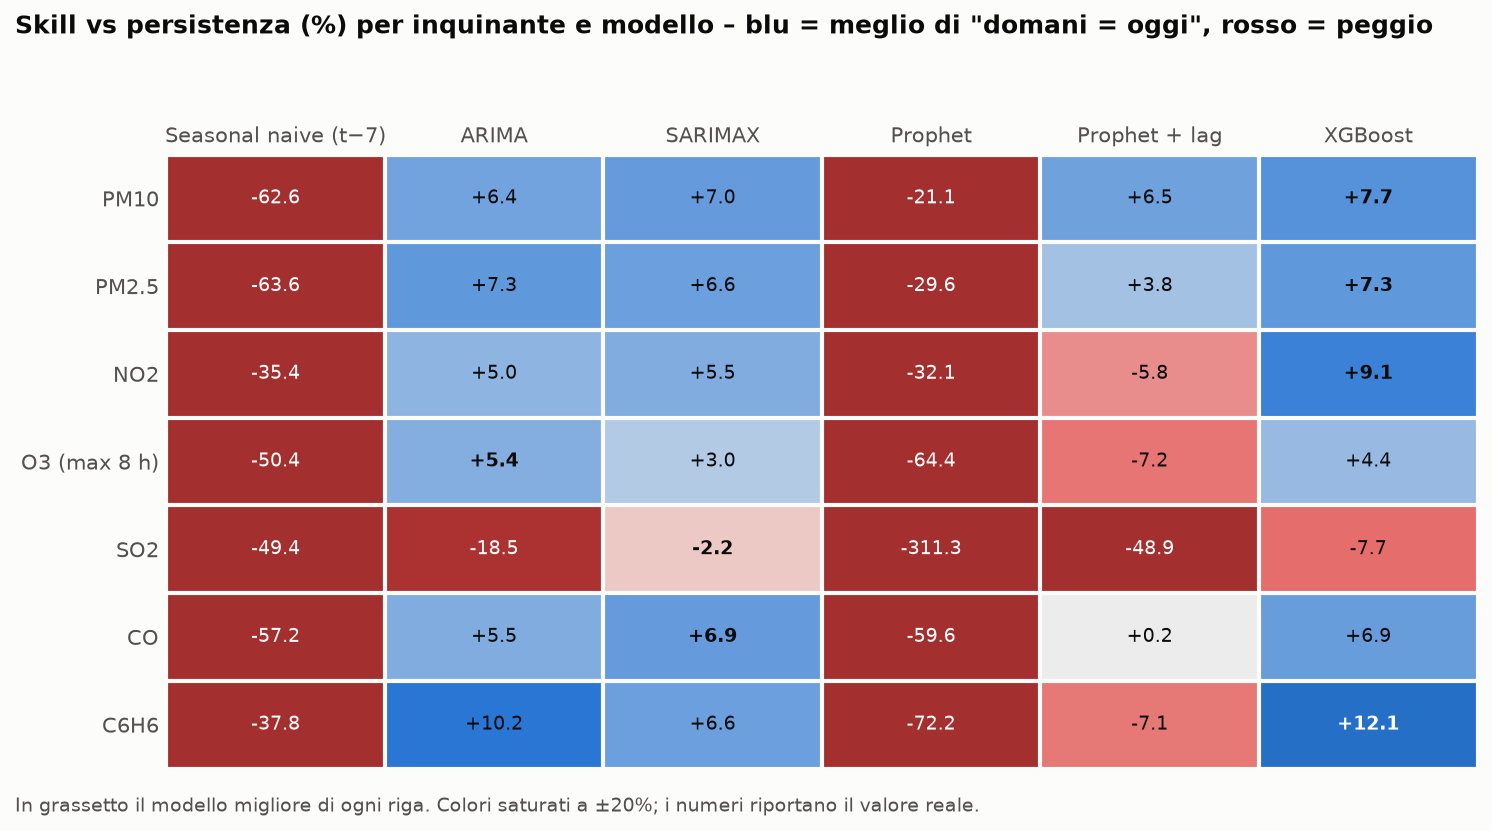
\includegraphics[width=0.9\textwidth]{11_skill_heatmap_pollutants.png}
  \caption{Skill rispetto alla persistenza per inquinante (4 stazioni aggregate) e modello. Blu: meglio di ``domani = oggi''; rosso: peggio. In grassetto il modello migliore di ogni riga.}
  \label{fig:fc_skill}
\end{figure}

\begin{table}[H]
  \centering
  \caption{Previsione a un giorno per inquinante (4 stazioni aggregate). MAE e media nell'unità dell'inquinante (\ugm; CO in \mgm).}
  \label{tab:fc_altri_skill}
  \small
  \begin{tabular}{l r r r l r r}
    \toprule
    \textbf{Inquinante} & \textbf{Giorni} & \textbf{Media} & \textbf{MAE pers.} & \textbf{Miglior modello} & \textbf{Skill} & \textbf{Prophet} \\
    \midrule
    PM10 & \num{1038} & 27,9 & 8,57 & XGBoost & $+7{,}7$\% & $-21{,}1$\% \\
    PM2,5 & \num{1025} & 13,8 & 4,55 & XGBoost / ARIMA & $+7{,}3$\% & $-29{,}6$\% \\
    NO\textsubscript{2} & \num{1087} & 34,2 & 7,70 & XGBoost & $+9{,}1$\% & $-32{,}1$\% \\
    O\textsubscript{3} (MDA8) & \num{1018} & 87,6 & 9,90 & ARIMA & $+5{,}4$\% & $-64{,}4$\% \\
    SO\textsubscript{2} & \num{1045} & 2,7 & 0,31 & nessuno$^{a}$ & -- & $-311{,}3$\% \\
    CO & \num{1064} & 0,57 & 0,122 & SARIMAX / XGBoost & $+6{,}9$\% & $-59{,}6$\% \\
    C\textsubscript{6}H\textsubscript{6} & 997 & 0,83 & 0,33 & XGBoost & $+12{,}1$\% & $-72{,}2$\% \\
    \bottomrule
    \multicolumn{7}{@{}l}{\footnotesize $^{a}$Nessun modello batte la persistenza (il migliore è SARIMAX, $-2{,}2$\%).}
  \end{tabular}
\end{table}

La Figura~\ref{fig:fc_skill} e la Tabella~\ref{tab:fc_altri_skill} mostrano che
il quadro del PM10 si ripete quasi identico per tutti gli inquinanti:
\begin{itemize}
  \item \textbf{la persistenza resta difficile da battere}: i modelli migliori
        fanno dal 5 al 12\% meglio di ``domani = oggi'', e per
        l'SO\textsubscript{2} nessun modello ci riesce;
  \item \textbf{ARIMA, SARIMAX e XGBoost sono vicini tra loro}: il migliore cambia
        da inquinante a inquinante e di solito lo scarto tra i primi tre è di 1--3
        punti di skill; fanno eccezione NO\textsubscript{2} e benzene, dove
        XGBoost si distacca un po' di più;
  \item \textbf{Prophet standard è sempre molto peggiore della persistenza} (da
        $-21$ a $-311$\%), e per O\textsubscript{3}, SO\textsubscript{2}, CO e
        benzene fa peggio anche della seasonal naive. Prophet + lag è competitivo
        solo per PM10 e PM2,5.
\end{itemize}

Le differenze tra inquinanti riflettono la loro natura.
\begin{itemize}
  \item \textbf{NO\textsubscript{2} e benzene: la skill più alta ($+9$ e $+12$\%).}
        Sono inquinanti legati al traffico, con un ciclo settimanale più marcato
        (Sezione~\ref{sec:temporale}): la seasonal naive è meno disastrosa che per
        gli altri inquinanti ($-35$ e $-38$\%, contro valori tra $-50$ e $-64$\%).
        XGBoost sfrutta il livello recente della stazione (medie a 7 e 30 giorni)
        e, in misura minore, il giorno della settimana, che ARIMA non utilizza.
  \item \textbf{O\textsubscript{3}: la skill più bassa tra gli inquinanti
        prevedibili ($+3$/$+5$\%).} L'MDA8 ha un ciclo stagionale fortissimo, ma le
        variazioni da un giorno all'altro dipendono da radiazione solare e
        temperatura, cioè dal meteo, che non è nel dataset. Prophet ottiene
        $-64$\%: la curva annuale sovradattata e il livello appreso negli anni di
        training non si ripetono nel 2026. Ad Ariano Irpino sovrastima (bias
        $+8{,}8$~\ugm), mentre a San Vitaliano e Volla sottostima (bias $-10$ e
        $-12$~\ugm); nella Figura~\ref{fig:fc_altri_test} Prophet resta sopra le
        osservazioni per tutto giugno e luglio ad Ariano.
  \item \textbf{SO\textsubscript{2}: nessun modello batte la persistenza.} Le
        concentrazioni, di 2--3~\ugm, sono vicine al limite di rilevabilità, e le
        serie sono dominate da cambi di livello irregolari, non stagionali. Ad
        Acerra, ad esempio, la media semestrale passa da \num{1.0}~\ugm\ (primo
        semestre 2023) a \num{5.1}~\ugm\ (secondo semestre 2026); è plausibile che
        si tratti in parte di derive strumentali. La persistenza segue questi
        gradini, mentre i modelli che tornano verso il livello del training (ARIMA
        con $d=0$, Prophet) li sbagliano. Prophet, inoltre, estrapola trend e
        stagionalità inesistenti ($-311$\%).
  \item \textbf{CO e benzene: buona skill, scarsa utilità pratica.} Le
        concentrazioni sono molto lontane dai limiti (il massimo giornaliero del CO
        nel test è circa la metà della soglia 2030 di 4~\mgm, e il benzene ha solo
        un limite annuale): la previsione è tecnicamente riuscita, ma non serve per
        le allerte.
\end{itemize}

\paragraph{Cambi di livello tra training e test.} Diverse serie hanno nel 2026 un
livello diverso da quello degli anni di training. A Napoli Ferrovia, ad esempio,
l'NO\textsubscript{2} è diminuito (media 2024 \num{52.8}~\ugm, media 2026
\num{42.6}~\ugm). I modelli che ricordano il livello del training lo sovrastimano
(bias $+3{,}2$~\ugm\ per ARIMA e SARIMAX, $+7{,}5$ per Prophet), mentre XGBoost, che
utilizza la media degli ultimi 30 giorni, ha un bias di $-0{,}75$ ed è il migliore
della stazione. È un ulteriore motivo per cui la persistenza e i modelli ancorati
ai valori recenti funzionano bene.

\begin{figure}[H]
  \centering
  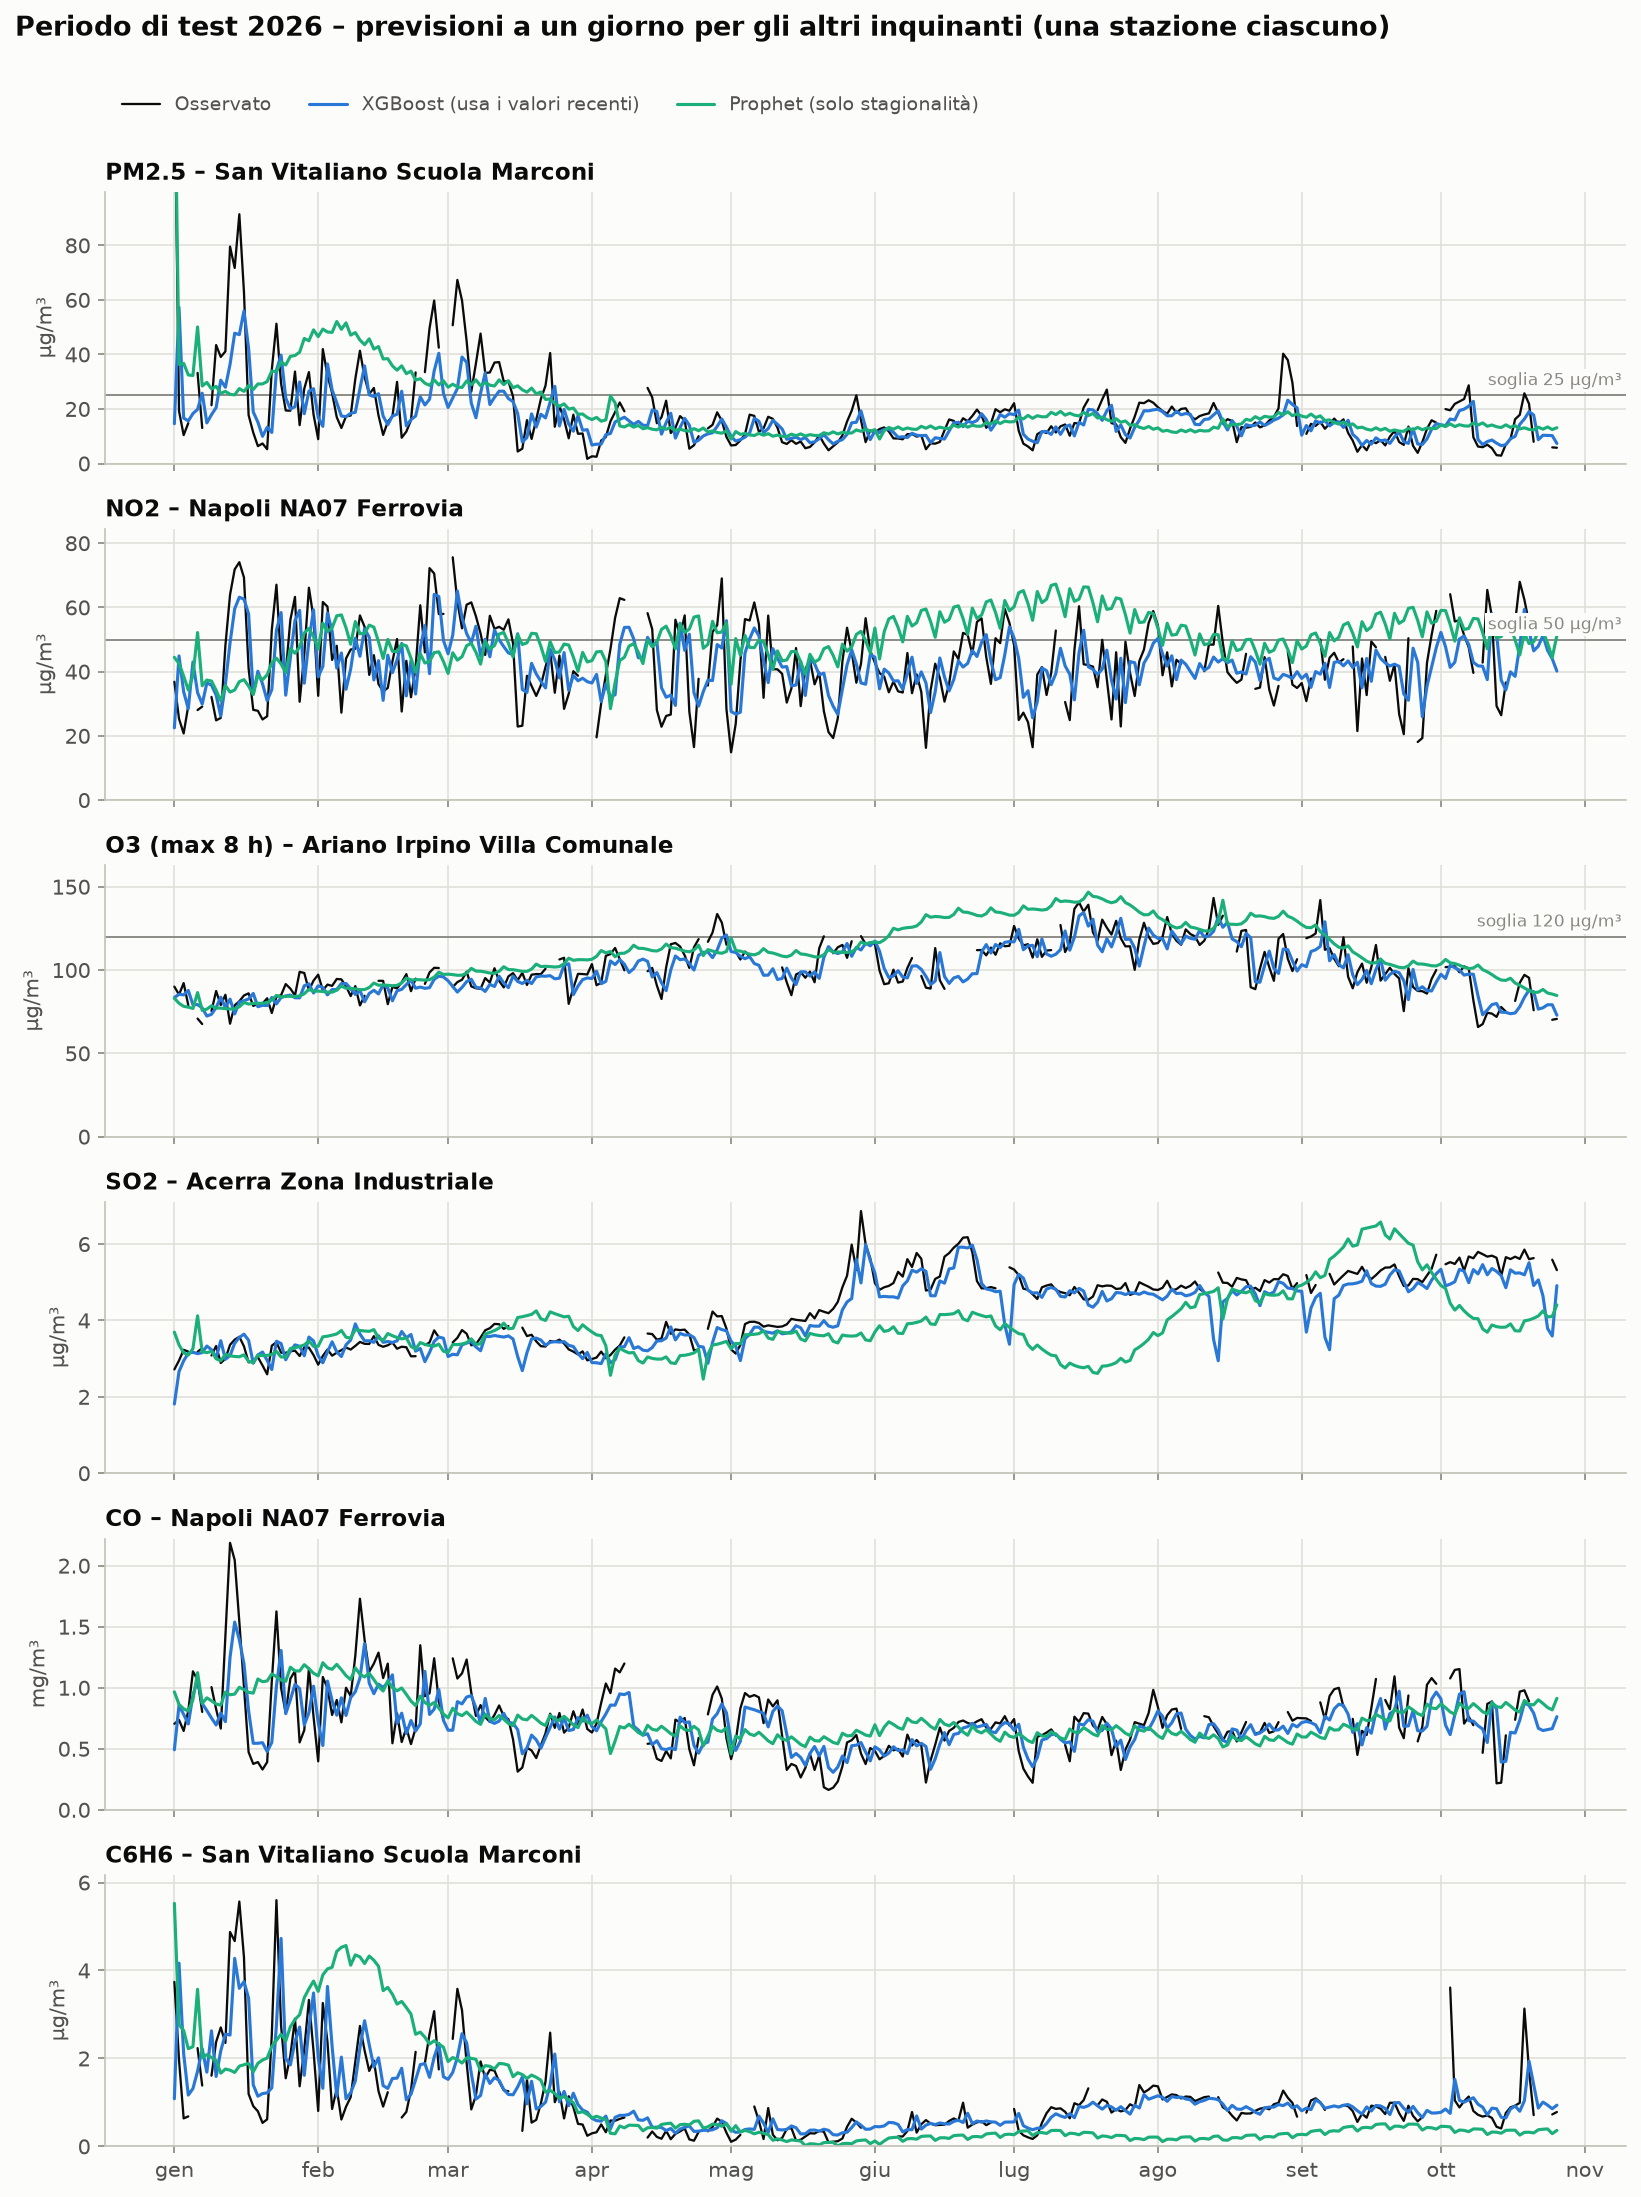
\includegraphics[width=0.9\textwidth]{12_forecast_other_pollutants.png}
  \caption{Periodo di test 2026: osservato (nero), XGBoost (blu) e Prophet standard (verde), una stazione per inquinante. La linea grigia indica la soglia dei superamenti, quando le concentrazioni le si avvicinano.}
  \label{fig:fc_altri_test}
\end{figure}

La Figura~\ref{fig:fc_altri_test} mostra gli stessi comportamenti osservati per il
PM10: XGBoost segue le osservazioni con un giorno di ritardo, mentre Prophet
disegna una curva stagionale. Sono visibili anche i problemi specifici: per
l'SO\textsubscript{2} ad Acerra Prophet scende a luglio mentre l'osservato resta
stabile intorno a 5~\ugm, e per il benzene a San Vitaliano Prophet sovrastima a
febbraio e sottostima per tutta l'estate, perché la curva annuale e il trend
appresi sul 2023--2025 non corrispondono al 2026.

Tra i risultati per stazione si segnalano:
\begin{itemize}
  \item Napoli Ferrovia, la stazione in cui i modelli guadagnano di più: PM10
        $+20$\% (XGBoost), PM2,5 $+18$\% (SARIMAX), benzene $+17$\% (XGBoost),
        NO\textsubscript{2} $+10$\% (XGBoost);
  \item NO\textsubscript{2} ad Avellino: SARIMAX $+16$\%;
  \item CO a Napoli NA06 Museo: SARIMAX $+15{,}5$\%;
  \item SO\textsubscript{2} ad Acerra e Polla, CO ad Acerra e PM2,5 ad Avellino:
        nessun modello batte davvero la persistenza.
\end{itemize}

\subsection{I superamenti}
\label{sec:fc_altri_superamenti}

\begin{figure}[H]
  \centering
  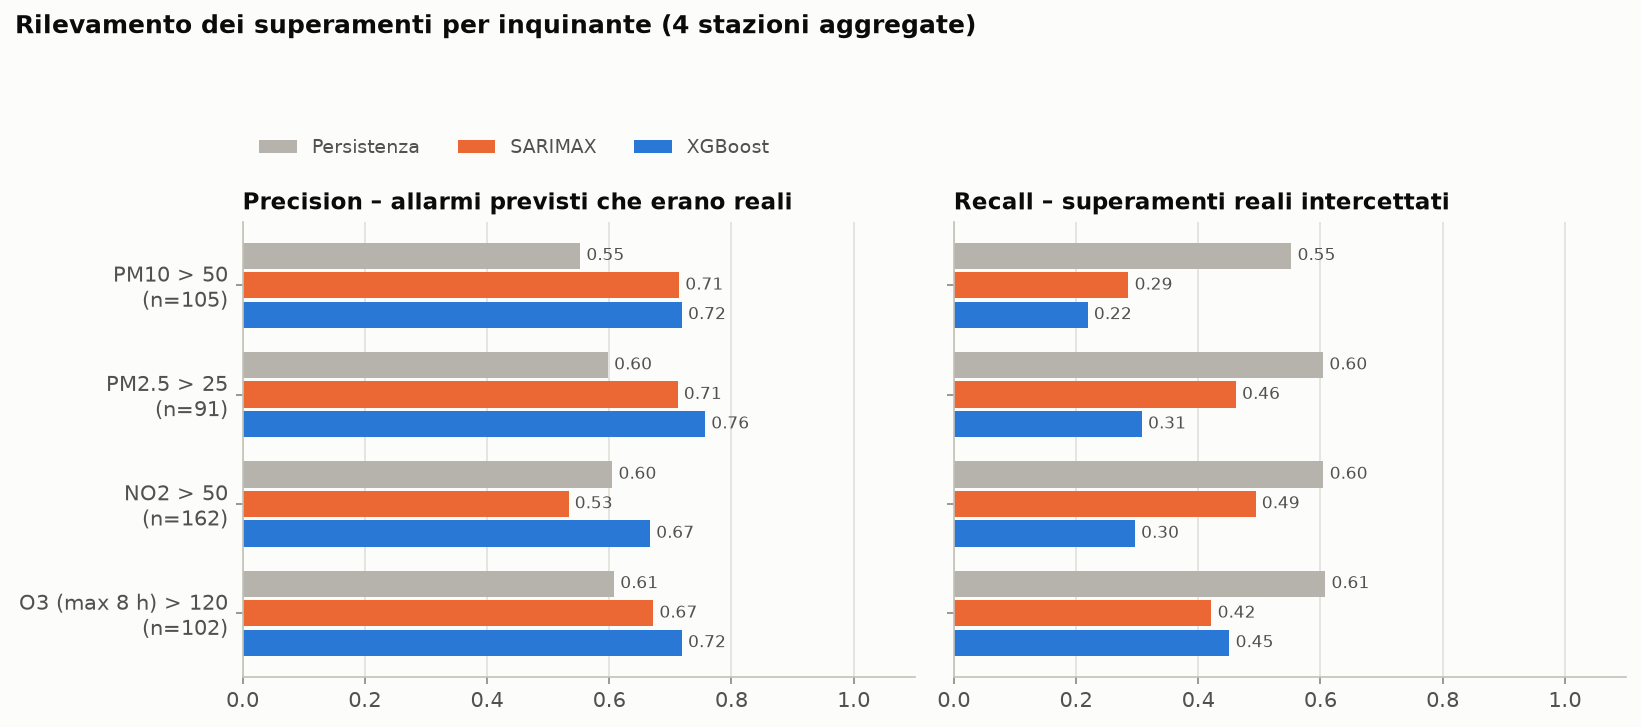
\includegraphics[width=0.9\textwidth]{14_exceedances_pollutants.png}
  \caption{Precision e recall sui superamenti per gli inquinanti con almeno 10 superamenti nel periodo di test (4 stazioni aggregate).}
  \label{fig:fc_superamenti}
\end{figure}

\begin{table}[H]
  \centering
  \caption{Superamenti nel periodo di test: persistenza e miglior F1 tra i modelli.}
  \label{tab:fc_superamenti}
  \small
  \begin{tabular}{l r c l}
    \toprule
    \textbf{Inquinante (soglia)} & \textbf{Superamenti} & \textbf{Persistenza: P / R / F1} & \textbf{Miglior F1 tra i modelli} \\
    \midrule
    PM10 ($>50$) & 105 & 0,55 / 0,55 / 0,55 & 0,41 (SARIMAX) \\
    PM2,5 ($>25$) & 91 & 0,60 / 0,60 / 0,60 & 0,56 (SARIMAX, Prophet + lag) \\
    NO\textsubscript{2} ($>50$) & 162 & 0,60 / 0,60 / 0,60 & 0,56 (ARIMA) \\
    O\textsubscript{3} MDA8 ($>120$) & 102 & 0,61 / 0,61 / 0,61 & 0,56 (ARIMA) \\
    \bottomrule
  \end{tabular}
\end{table}

La conclusione della Sezione~\ref{sec:fc_picchi} vale per tutti gli inquinanti
(Figura~\ref{fig:fc_superamenti} e Tabella~\ref{tab:fc_superamenti}): \textbf{i
modelli hanno precision più alta ma recall più bassa della persistenza}, e la
persistenza ha l'F1 migliore per ogni inquinante. Le cause sono le stesse: attrazione
verso la media, riconversione dalla scala logaritmica e assenza del meteo.

Per PM2,5, NO\textsubscript{2} e O\textsubscript{3} il divario è però più piccolo che
per il PM10: la recall di ARIMA e SARIMAX arriva a \num{0.42}--\num{0.49}, contro
\num{0.23}--\num{0.29} per il PM10, mentre XGBoost, più prudente, resta più basso
(\num{0.30}--\num{0.45}). Per questi inquinanti la soglia è più vicina ai livelli
tipici: a Napoli Ferrovia, ad esempio, l'NO\textsubscript{2} supera 50~\ugm\ in 78
giorni su 269, e ad Ariano Irpino l'O\textsubscript{3} supera 120~\ugm\ in 33 giorni
su 262. Molti superamenti sono quindi giorni ``ordinari'' e non picchi estremi, e un
modello che si mantiene vicino alla media li intercetta comunque.

Con le soglie 2030, il numero di superamenti di PM2,5 e NO\textsubscript{2}
costituirebbe già oggi un problema normativo: la nuova direttiva ne ammetterà al
massimo 18 all'anno per stazione~\cite{direttiva2024}.

\subsection{Cosa guida la previsione}
\label{sec:fc_altri_importanza}

\begin{figure}[H]
  \centering
  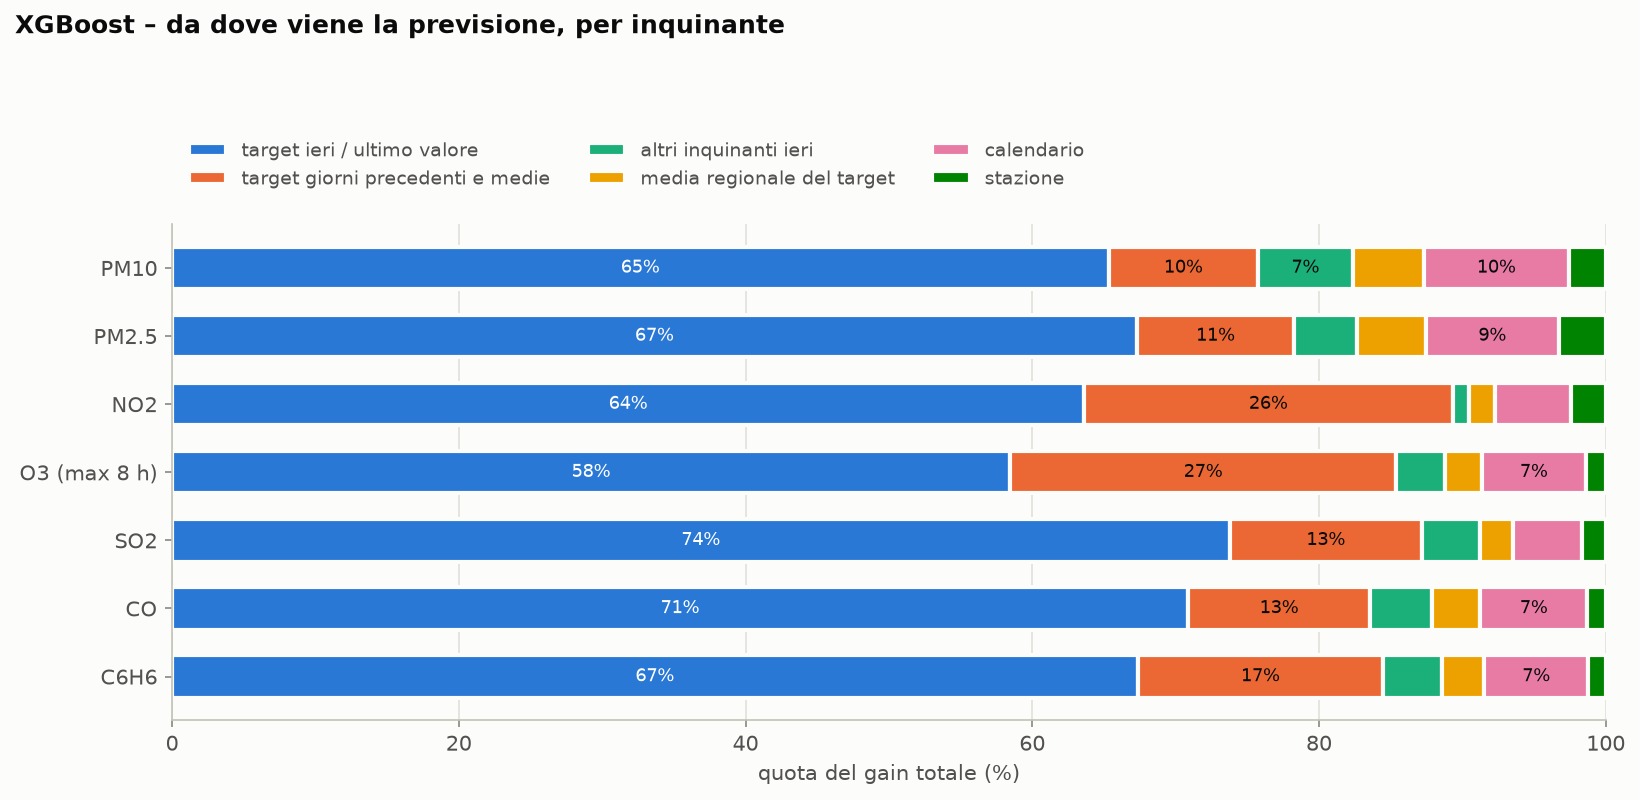
\includegraphics[width=0.9\textwidth]{13_xgb_importance_groups.png}
  \caption{Quota del \emph{gain} totale di XGBoost per gruppo di feature e inquinante.}
  \label{fig:fc_imp_gruppi}
\end{figure}

Per tutti gli inquinanti (Figura~\ref{fig:fc_imp_gruppi}) dal \textbf{75 al 90\%}
del potere predittivo proviene dai valori recenti del target stesso; il valore del
giorno precedente e l'ultimo valore osservato pesano da soli il 58--74\%. Gli altri
inquinanti, il segnale regionale, il calendario e la stazione contribuiscono per
pochi punti ciascuno.

Le differenze riguardano la \textbf{memoria} della serie:
\begin{itemize}
  \item per \textbf{NO\textsubscript{2} e O\textsubscript{3}} circa un quarto del
        gain (26--27\%) proviene dalle medie a 7 e 30 giorni e dai giorni
        precedenti: l'NO\textsubscript{2} dipende dal livello tipico della stazione
        e dal traffico della settimana, l'O\textsubscript{3} da un livello di fondo
        regionale che varia lentamente con la stagione;
  \item per gli altri inquinanti i giorni precedenti e le medie pesano solo il
        10--17\%, e quasi tutto dipende dal giorno precedente (65--74\%). Il caso
        estremo è l'SO\textsubscript{2} (74\%): con serie che cambiano livello a
        gradini, il valore di ieri è la migliore stima del livello attuale.
\end{itemize}

Il messaggio è lo stesso del PM10: \textbf{senza dati meteorologici, la previsione
di qualunque inquinante è ``il valore di ieri, corretto''}.

% ------------------------------------------------------------
\section{Previsione a sette giorni}
\label{sec:fc_7giorni}

Finora la domanda era ``quanto sarà domani?''. In questa sezione si valuta quanto
si riesce a prevedere \textbf{fino a una settimana prima}, in due parti:
\begin{enumerate}
  \item una valutazione su tutto il 2026 a orizzonti da 1 a 7 giorni;
  \item una previsione vera e propria per i 7 giorni successivi all'ultimo dato del
        dataset (27 ottobre -- 2 novembre 2026).
\end{enumerate}

\subsection{Previsione a $h$ giorni}
L'\textbf{orizzonte $h$} è il numero di giorni tra l'ultimo dato utilizzato e il
giorno previsto: prevedere il giorno $t$ con $h=7$ significa utilizzare solo i dati
fino a $t-7$, come se la previsione fosse emessa una settimana prima; $h=1$ è la
previsione a un giorno delle sezioni precedenti. Valutazione, periodi e parametri
restano quelli della Sezione~\ref{sec:fc_valutazione}: ogni modello è stimato una
sola volta sul training e non viene ristimato durante il test. La
Tabella~\ref{tab:fc_h} descrive come ciascun modello produce la previsione a $h$
giorni.

\begin{table}[H]
  \centering
  \caption{Previsione a $h$ giorni nei diversi modelli.}
  \label{tab:fc_h}
  \small
  \begin{tabularx}{\textwidth}{@{}>{\raggedright\arraybackslash}p{3cm} X@{}}
    \toprule
    \textbf{Modello} & \textbf{Previsione a $h$ giorni} \\
    \midrule
    Persistenza & Ultimo valore noto al giorno $t-h$ \\
    \addlinespace
    Seasonal naive ($t-7$) & Valore del giorno $t-7$, noto per ogni $h \le 7$; a $h=7$ coincide quindi con la persistenza \\
    \addlinespace
    ARIMA / SARIMAX & \textbf{Ricorsiva}: dal giorno di origine il modello prevede il giorno successivo, utilizza quella previsione come se fosse un dato osservato, e così via per 7 passi, con gli stessi parametri della previsione a un giorno \\
    \addlinespace
    Prophet & Nessuna modifica: non utilizza i dati recenti, quindi prevede lo stesso valore a qualunque orizzonte \\
    \addlinespace
    Prophet + lag, XGBoost & \textbf{Diretta}: un modello separato per ogni $h$, con tutte le feature spostate di $h$ giorni. Per $h=7$ XGBoost utilizza i valori di $t-7$, $t-8$, $t-9$ e $t-14$, le medie a 7 e 30 giorni che terminano a $t-7$ e gli altri inquinanti di $t-7$. Le feature di calendario si riferiscono al giorno previsto, noto in anticipo \\
    \bottomrule
  \end{tabularx}
\end{table}

Per confrontare gli orizzonti in modo equo, le metriche sono calcolate su un
\textbf{campione comune}: i giorni-stazione con osservazione valida e previsione a
tutti e 7 gli orizzonti (per il PM10, gli stessi \num{1038} giorni-stazione della
Sezione~\ref{sec:fc_risultati}). La \textbf{skill} è sempre calcolata rispetto alla
persistenza \textbf{allo stesso orizzonte}: la skill a 7 giorni indica quindi quanto
un modello batte ``fra una settimana = oggi''.

\subsection{Come cresce l'errore}
\label{sec:fc_errore_h}

\begin{figure}[H]
  \centering
  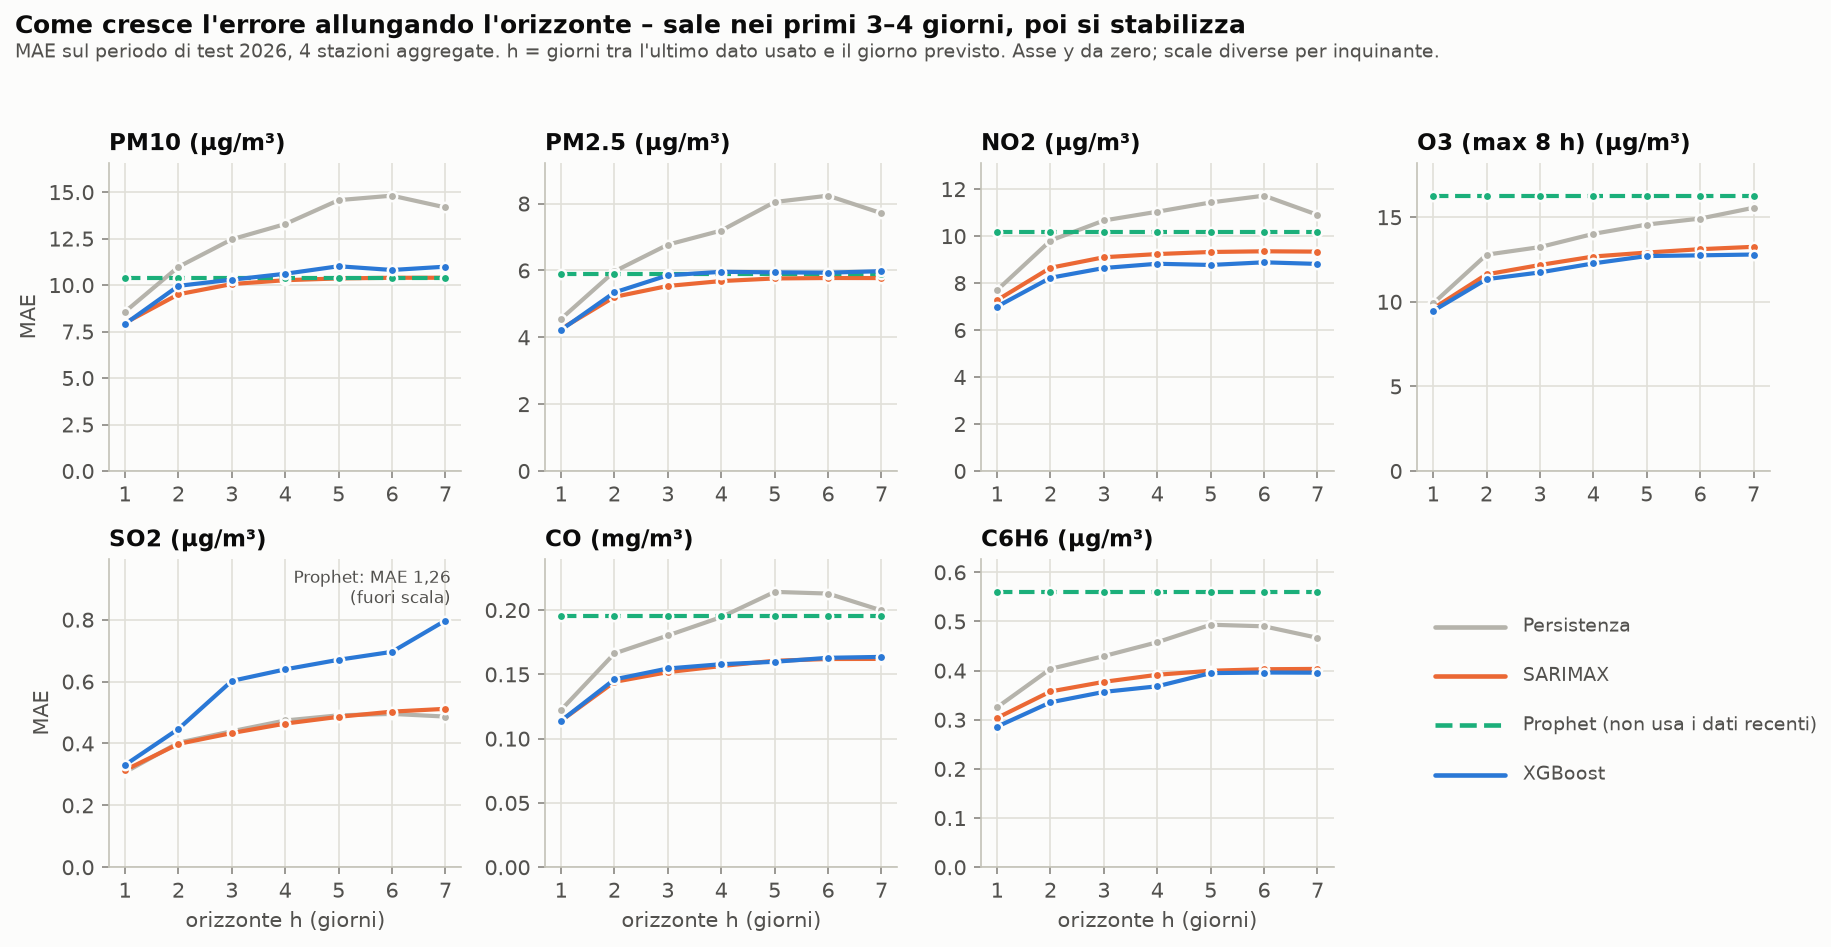
\includegraphics[width=0.9\textwidth]{15_mae_by_horizon.png}
  \caption{MAE sul periodo di test 2026 (4 stazioni aggregate) in funzione dell'orizzonte, per persistenza, SARIMAX, Prophet (tratteggiato) e XGBoost.}
  \label{fig:fc_mae_h}
\end{figure}

\begin{table}[H]
  \centering
  \caption{MAE della persistenza a $h=1$ e $h=7$ e miglior modello a $h=7$ (\ugm; CO in \mgm).}
  \label{tab:fc_mae_h}
  \footnotesize
  \setlength{\tabcolsep}{4pt}
  \begin{tabular}{l r r l r r r}
    \toprule
    \textbf{Inquinante} & \textbf{Pers. $h$=1} & \textbf{Pers. $h$=7} & \textbf{Miglior a $h$=7} & \textbf{MAE} & \textbf{Skill} & \textbf{Prophet} \\
    \midrule
    PM10 & 8,57 & 14,18 & Prophet / SARIMAX & 10,37 / 10,40 & $+26{,}8$ / $+26{,}7$\% & 10,37 \\
    PM2,5 & 4,55 & 7,71 & ARIMA & 5,70 & $+26{,}1$\% & 5,90 \\
    NO\textsubscript{2} & 7,70 & 10,91 & XGBoost & 8,82 & $+19{,}2$\% & 10,17 \\
    O\textsubscript{3} & 9,90 & 15,56 & XGBoost & 12,80 & $+17{,}8$\% & 16,27 \\
    SO\textsubscript{2} & 0,31 & 0,49 & Persistenza & 0,49 & -- & 1,26 \\
    CO & 0,122 & 0,200 & SARIMAX & 0,162 & $+18{,}9$\% & 0,195 \\
    C\textsubscript{6}H\textsubscript{6} & 0,33 & 0,47 & ARIMA & 0,36 & $+23{,}1$\% & 0,56 \\
    \bottomrule
  \end{tabular}
\end{table}

Dalla Figura~\ref{fig:fc_mae_h} e dalla Tabella~\ref{tab:fc_mae_h} emerge che:
\begin{itemize}
  \item \textbf{l'errore cresce soprattutto nei primi 2--3 giorni, poi si
        stabilizza}. Per il PM10 il MAE di SARIMAX passa da \num{7.97} a
        \num{10.06} a $h=3$ e arriva a \num{10.40} a $h=7$: l'86\% dell'aumento
        avviene entro il terzo giorno. Per PM2,5 e NO\textsubscript{2} il quadro è
        lo stesso (88--90\%). L'O\textsubscript{3} fa eccezione: il MAE continua a
        crescere fino al settimo giorno (XGBoost: \num{9.46}, \num{11.74},
        \num{12.80} a $h=1$, 3 e 7);
  \item \textbf{la persistenza peggiora molto di più}: per il PM10 il suo MAE
        cresce del 65\% (da \num{8.57} a \num{14.18}), quello di SARIMAX del 30\%.
        Per questo la skill dei modelli \textbf{cresce} con l'orizzonte, da
        $+6$/$+8$\% a un giorno a $+22$/$+27$\% a sette giorni. Ciò non significa
        che i modelli migliorino, ma che ``fra una settimana = oggi'' è una
        previsione pessima;
  \item \textbf{per PM10 e PM2,5, dopo 3--4 giorni i modelli non fanno meglio della
        stagionalità}: da $h=4$ in poi ARIMA, SARIMAX e XGBoost hanno un errore
        entro il 5\% di quello di Prophet standard, che non utilizza alcun dato
        recente. A $h=7$ per il PM10 il migliore è proprio Prophet (\num{10.37}),
        con SARIMAX praticamente pari (\num{10.40}). A una settimana, i dati
        recenti non dicono quasi più nulla sul particolato: resta la media
        stagionale della stazione;
  \item \textbf{per NO\textsubscript{2}, O\textsubscript{3}, CO e benzene i dati
        recenti servono anche a sette giorni}: a $h=7$ il miglior modello ha un MAE
        inferiore a quello di Prophet del 13\% per l'NO\textsubscript{2}, del 17\%
        per il CO, del 21\% per l'O\textsubscript{3} e del 36\% per il benzene.
        Prophet sbaglia infatti il \emph{livello} di questi inquinanti nel 2026
        (il calo dell'NO\textsubscript{2} a Napoli e l'estrapolazione della curva
        annuale per O\textsubscript{3} e benzene,
        Sezione~\ref{sec:fc_altri_skill}), mentre i modelli che conoscono la media
        degli ultimi 30 giorni si correggono. XGBoost lo conferma: a $h=7$ la
        feature più importante è la media a 30 giorni per 5 inquinanti su 7 (per
        l'NO\textsubscript{2} è la seconda, dopo la stazione), seguita da stazione
        e calendario, mentre il valore del giorno precedente, dominante a un
        giorno, scompare. A una settimana contano \textbf{il livello recente e la
        stagione}, non la dinamica del giorno prima;
  \item \textbf{SARIMAX non ripaga a orizzonti lunghi}: contrariamente a quanto ci
        si poteva aspettare (Sezione~\ref{sec:fc_sarimax}), a $h=7$ SARIMAX e
        ARIMA sono quasi equivalenti per PM10 (\num{10.40} contro \num{10.43}),
        PM2,5 e O\textsubscript{3}; SARIMAX è leggermente migliore per il CO
        (\num{0.162} contro \num{0.169}) e peggiore per il benzene. Un ciclo
        settimanale debole e una stagionalità annuale lenta non bastano a ridurre
        l'errore;
  \item \textbf{per l'SO\textsubscript{2} la persistenza resta il miglior modello a
        ogni orizzonte}: SARIMAX la eguaglia (entro $\pm5$\%), mentre ARIMA e
        XGBoost peggiorano rapidamente (a $h=7$ XGBoost ha un MAE di \num{0.80}
        contro \num{0.49}). Con serie a gradini, l'ultimo livello osservato è la
        stima migliore anche una settimana dopo.
\end{itemize}

\subsection{L'effetto dell'orizzonte sulla previsione}

\begin{figure}[H]
  \centering
  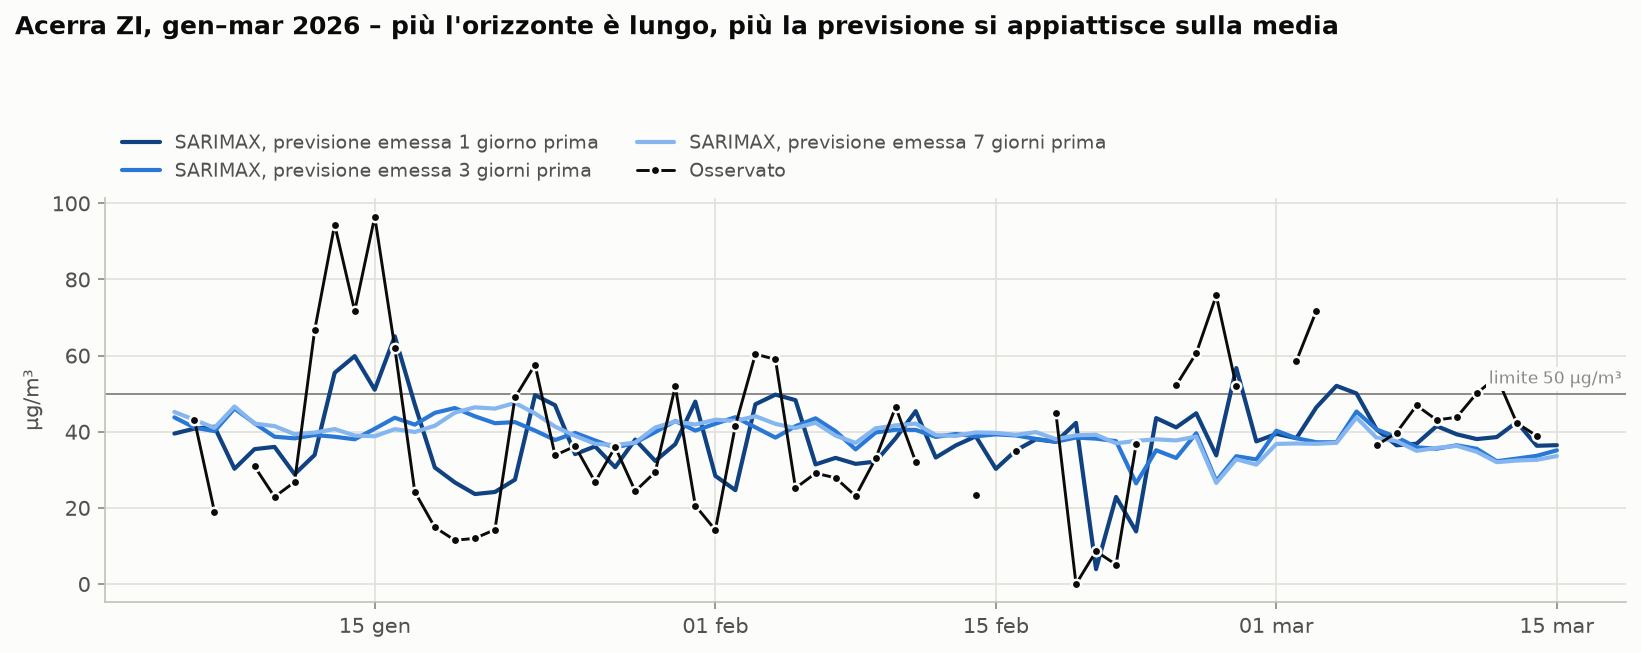
\includegraphics[width=0.9\textwidth]{16_zoom_horizons_acerra.png}
  \caption{PM10 ad Acerra, gennaio--marzo 2026: osservato (punti neri) e previsione SARIMAX emessa 1 giorno (blu scuro), 3 giorni (blu) e 7 giorni prima (azzurro).}
  \label{fig:fc_zoom_h}
\end{figure}

Nella Figura~\ref{fig:fc_zoom_h} la previsione a un giorno segue le osservazioni con
il ritardo di un giorno già visto nella Sezione~\ref{sec:fc_risultati}. Le
previsioni a 3 e 7 giorni sono quasi sovrapposte e quasi piatte, intorno a
35--\SI{45}{\micro\gram\per\cubic\metre}, il livello invernale tipico di Acerra.
L'episodio di metà gennaio (oltre \SI{90}{\micro\gram\per\cubic\metre}) e quello di
fine febbraio \textbf{non lasciano traccia} nelle previsioni a più giorni, e anche
il crollo di metà febbraio (sotto \SI{10}{\micro\gram\per\cubic\metre}) passa
inosservato. È la stessa attrazione verso la media della
Sezione~\ref{sec:fc_picchi}, ma molto più forte: senza informazioni sul meteo dei
giorni futuri, l'unica previsione ``sicura'' a una settimana è la media.

\subsection{I superamenti con anticipo}

\begin{figure}[H]
  \centering
  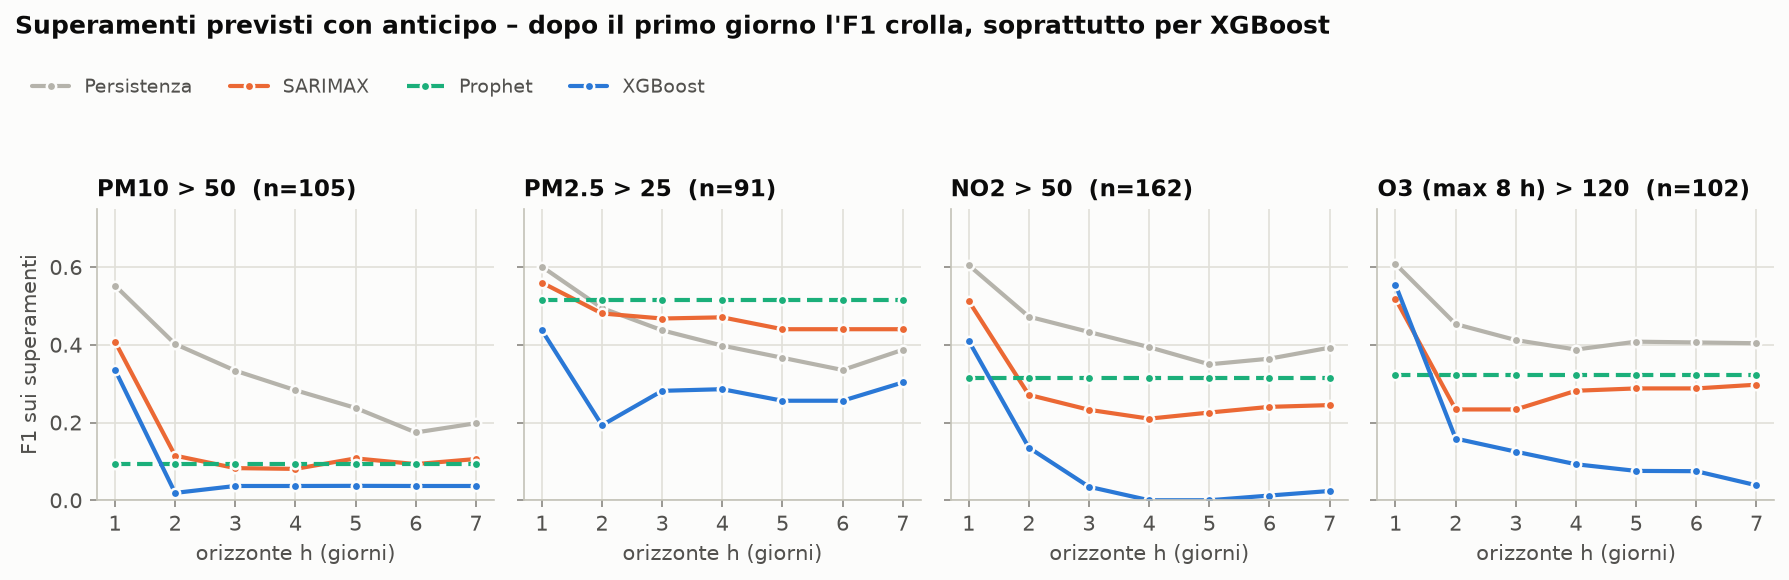
\includegraphics[width=0.9\textwidth]{17_exceedance_f1_by_horizon.png}
  \caption{F1 sui superamenti in funzione dell'orizzonte, per i quattro inquinanti con superamenti nel periodo di test (4 stazioni aggregate).}
  \label{fig:fc_f1_h}
\end{figure}

Già a un giorno i modelli intercettano pochi superamenti
(Sezione~\ref{sec:fc_picchi}); a più giorni la situazione peggiora rapidamente
(Figura~\ref{fig:fc_f1_h}):
\begin{itemize}
  \item \textbf{XGBoost e ARIMA non prevedono quasi più superamenti dopo il primo
        giorno}: per PM10 e NO\textsubscript{2} l'F1 di XGBoost scende sotto
        \num{0.05} da $h=2$ o 3 in poi; quello di ARIMA è già vicino a zero da $h=2$
        per il PM10 e scende fino a \num{0.01} a $h=7$ per l'NO\textsubscript{2}.
        Prevedere sempre valori vicini alla media minimizza l'errore assoluto, ma
        porta a non superare mai la soglia;
  \item \textbf{per PM10, NO\textsubscript{2} e O\textsubscript{3} le baseline
        restano le migliori a ogni orizzonte}: vince la persistenza o, in alcuni
        casi, la seasonal naive. Anche le baseline, però, perdono valore: per il
        PM10 l'F1 della persistenza scende da \num{0.55} a \num{0.20} in una
        settimana;
  \item \textbf{il PM2,5 fa eccezione}: Prophet (\num{0.51}) e Prophet + lag
        (\num{0.49}--\num{0.53}) battono la persistenza da $h=2$, SARIMAX
        (\num{0.44}--\num{0.47}) da $h=3$, mentre la persistenza scende a
        \num{0.34}--\num{0.49}. I superamenti di PM2,5 sopra 25~\ugm\ sono
        concentrati nei mesi invernali (Sezione~\ref{sec:temporale}), e una
        previsione stagionale che resta sopra la soglia per tutto l'inverno ne
        intercetta una buona parte. Si tratta di un'``allerta di stagione'', non di
        episodio.
\end{itemize}

Con questi dati, quindi, \textbf{non è possibile costruire un'allerta di
superamento con alcuni giorni di anticipo}: servono le previsioni meteorologiche
(Sezione~\ref{sec:fc_conclusioni}).

\subsection{Previsione per il periodo 27 ottobre -- 2 novembre 2026}
La previsione è emessa con i dati fino al \textbf{26 ottobre 2026}, ultimo giorno
del dataset. Per ogni inquinante si utilizza il modello con il MAE medio più basso
sui 7 orizzonti nel periodo di test: SARIMAX per PM10 e CO, ARIMA per PM2,5 e
benzene, XGBoost per NO\textsubscript{2} e O\textsubscript{3} e la persistenza per
l'SO\textsubscript{2}.

L'\textbf{intervallo all'80\%} è empirico: per ogni orizzonte si prendono il 10° e il
90° percentile degli errori commessi dal modello nel 2026 (in scala logaritmica,
sulle 4 stazioni insieme) e si applicano alla previsione. L'intervallo è quindi più
ampio a $h=7$ che a $h=1$, e asimmetrico verso l'alto.

\begin{figure}[H]
  \centering
  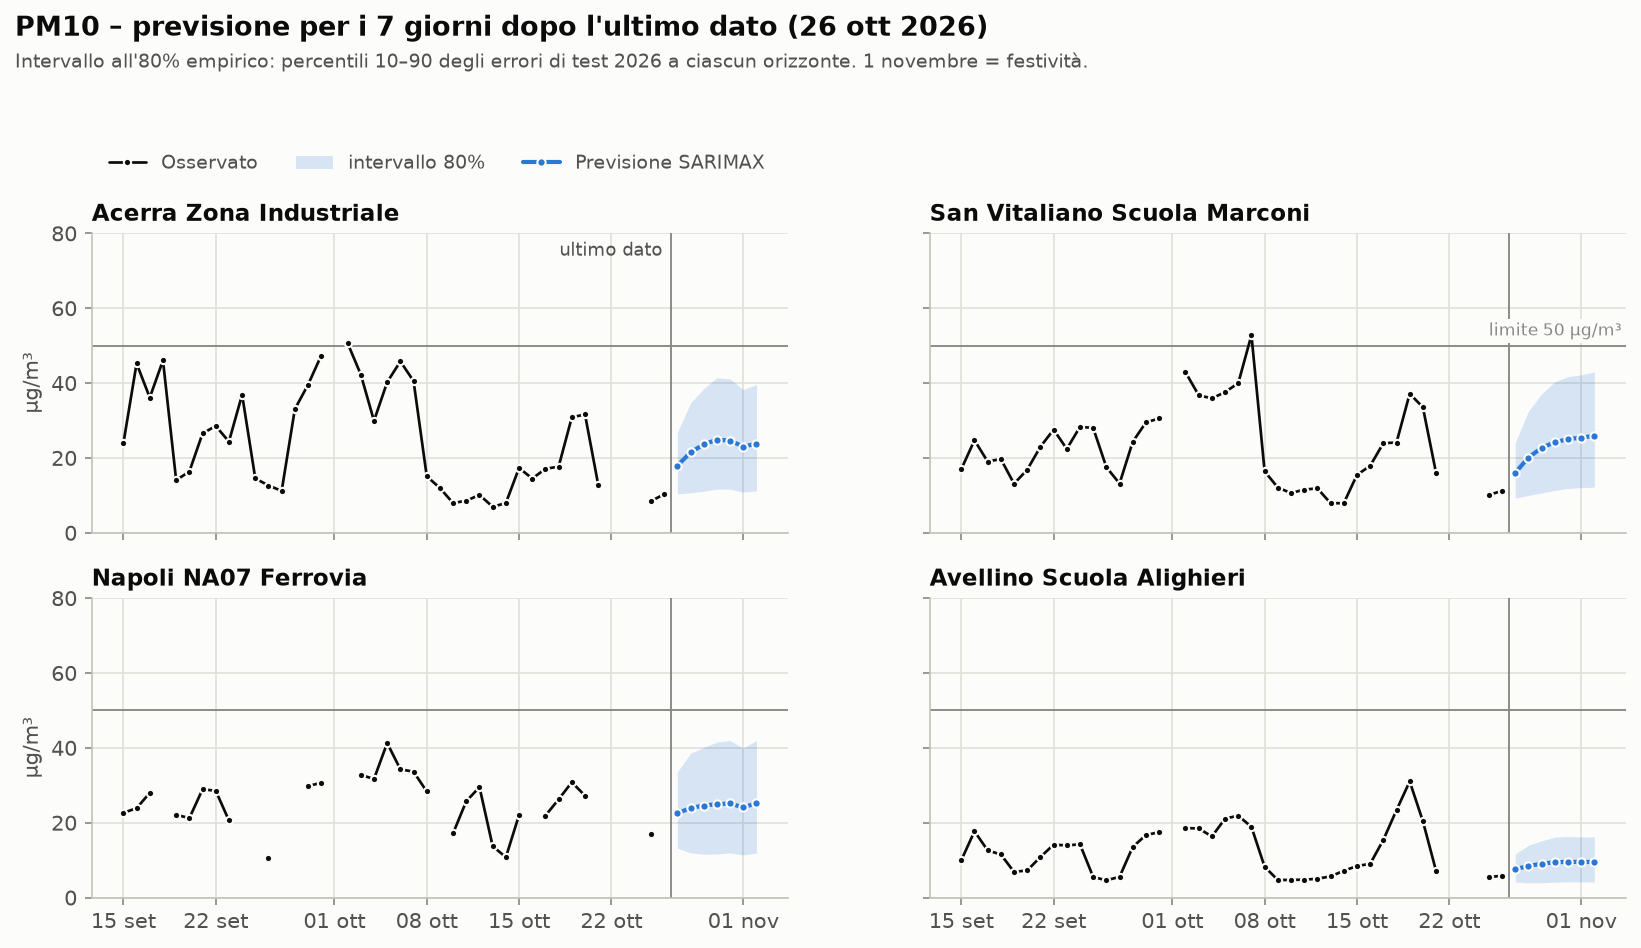
\includegraphics[width=0.9\textwidth]{18_next7_pm10.png}
  \caption{PM10: ultime sei settimane osservate (nero) e previsione SARIMAX per i 7 giorni successivi (blu), con intervallo all'80\% (banda azzurra).}
  \label{fig:fc_next7}
\end{figure}

\begin{table}[H]
  \centering
  \caption{Previsione SARIMAX del PM10 (\ugm) per i 7 giorni successivi all'ultimo dato; tra parentesi l'intervallo all'80\%.}
  \label{tab:fc_next7}
  \small
  \begin{tabular}{l c c c c}
    \toprule
    \textbf{Giorno} & \textbf{Acerra ZI} & \textbf{San Vitaliano} & \textbf{Napoli Ferrovia} & \textbf{Avellino} \\
    \midrule
    Ultimo dato & 10 (26/10) & 11 (26/10) & 17 (25/10) & 6 (26/10) \\
    \midrule
    mar 27 ott & 18 (10--27) & 16 (9--24) & 23 (13--34) & 8 (4--12) \\
    mer 28 ott & 21 (11--35) & 20 (10--32) & 24 (12--39) & 8 (4--14) \\
    gio 29 ott & 24 (11--39) & 23 (11--37) & 25 (12--40) & 9 (4--15) \\
    ven 30 ott & 25 (12--41) & 24 (11--40) & 25 (12--42) & 9 (4--16) \\
    sab 31 ott & 25 (12--41) & 25 (12--42) & 25 (12--42) & 10 (4--16) \\
    dom 1 nov & 23 (11--38) & 25 (12--42) & 24 (11--40) & 10 (4--16) \\
    lun 2 nov & 24 (11--40) & 26 (12--43) & 25 (12--42) & 10 (4--16) \\
    \bottomrule
  \end{tabular}
\end{table}

\paragraph{PM10.} Il 25 e 26 ottobre i valori erano bassi
(6--\SI{17}{\micro\gram\per\cubic\metre}). La previsione
(Figura~\ref{fig:fc_next7} e Tabella~\ref{tab:fc_next7}) risale in 3--4 giorni
verso il livello tipico di fine ottobre: circa
\SI{25}{\micro\gram\per\cubic\metre} nelle tre stazioni dell'area napoletana e circa
10 ad Avellino. Non è previsto alcun superamento: anche l'estremo superiore
dell'intervallo (40--\SI{43}{\micro\gram\per\cubic\metre}) resta sotto 50. La
risalita verso la media è quella già osservata nella Figura~\ref{fig:fc_zoom_h}: il
modello non ``sa'' se l'aria pulita durerà e torna quindi verso il valore
stagionale. Il 1° novembre (festivo) si osserva un piccolo calo ad Acerra.

\paragraph{Gli altri inquinanti.} Le previsioni sono riassunte nella
Tabella~\ref{tab:fc_next7_altri}.

\begin{table}[H]
  \centering
  \caption{Previsione per gli altri inquinanti, 27 ottobre -- 2 novembre 2026.}
  \label{tab:fc_next7_altri}
  \small
  \begin{tabularx}{\textwidth}{@{}l X >{\raggedright\arraybackslash}p{4cm}@{}}
    \toprule
    \textbf{Inquinante} & \textbf{Previsione} & \textbf{Soglia} \\
    \midrule
    NO\textsubscript{2} & Napoli Ferrovia 42--49~\ugm\ (intervallo fino a 71); Acerra 35--42~\ugm & 50~\ugm: superamento possibile in entrambe \\
    \addlinespace
    PM2,5 & Napoli 15~\ugm; altre stazioni 6--11~\ugm & 25~\ugm: sotto la soglia \\
    \addlinespace
    O\textsubscript{3} & 61--77~\ugm & 120~\ugm: molto sotto (autunno) \\
    \addlinespace
    SO\textsubscript{2}, CO, benzene & Valori bassi e stabili & -- \\
    \bottomrule
  \end{tabularx}
\end{table}

Al momento della stesura questi sette giorni sono già trascorsi, ma i dati validati
non sono ancora disponibili nel dataset: il confronto con le osservazioni sarà la
prima verifica da effettuare quando lo saranno.

% ------------------------------------------------------------
\section{Conclusioni}
\label{sec:fc_conclusioni}

L'analisi di forecasting ha evidenziato i seguenti risultati principali:
\begin{itemize}
  \item \textbf{la scelta dell'algoritmo conta meno dell'informazione
        disponibile}: per il PM10, ARIMA, SARIMAX, Prophet + lag e XGBoost
        raggiungono quasi la stessa accuratezza (MAE di circa
        \SI{8}{\micro\gram\per\cubic\metre}) e battono ``domani = oggi'' solo del
        6--8\%; per gli altri inquinanti il guadagno è tra il 5 e il 12\%, e i
        modelli migliori sono di nuovo vicini tra loro;
  \item \textbf{la persistenza è il segnale dominante} per il giorno successivo,
        per tutti gli inquinanti: un modello che ignora i valori recenti, come
        Prophet standard, a un giorno è sempre peggiore della persistenza. A più
        giorni la persistenza perde valore, e per PM10, PM2,5 e NO\textsubscript{2}
        Prophet la supera già a 2--3 giorni di anticipo;
  \item \textbf{la stagionalità e il ciclo settimanale sono reali ma secondari} a
        un orizzonte di un giorno; il ciclo settimanale conta un po' di più per gli
        inquinanti da traffico (NO\textsubscript{2}, benzene);
  \item \textbf{così come sono, i modelli non sono adatti alle allerte per
        superamento}: hanno una buona precision ma mancano da metà a tre quarti dei
        superamenti, e per ogni inquinante la persistenza ha un F1 migliore;
  \item \textbf{a più giorni l'errore cresce soprattutto nei primi 2--3 giorni,
        poi si stabilizza}. La skill rispetto alla persistenza aumenta (da $+15$ a
        $+27$\% a sette giorni), ma solo perché la persistenza peggiora molto più
        rapidamente. Per PM10 e PM2,5, oltre il terzo o quarto giorno i modelli non
        battono più la sola stagionalità di Prophet; per NO\textsubscript{2},
        O\textsubscript{3}, CO e benzene il livello recente (media a 30 giorni)
        resta invece utile anche a una settimana;
  \item \textbf{con questi dati non è possibile emettere allerte con alcuni giorni
        di anticipo}: dopo il primo giorno l'F1 sui superamenti crolla,
        soprattutto per XGBoost e ARIMA; l'unica eccezione parziale è il PM2,5, i
        cui superamenti invernali sono in buona parte stagionali;
  \item \textbf{la previsione ha senso pratico} per PM10, PM2,5,
        NO\textsubscript{2} e O\textsubscript{3}, che presentano superamenti
        frequenti; per SO\textsubscript{2} e CO, con valori molto sotto i limiti, e
        per il benzene, che ha solo un limite annuale, la previsione giornaliera ha
        scarsa utilità operativa.
\end{itemize}

\subsection{Sviluppi futuri}
La Tabella~\ref{tab:fc_sviluppi} riporta i possibili sviluppi, in ordine di impatto
atteso.

\begin{table}[H]
  \centering
  \caption{Sviluppi futuri, in ordine di impatto atteso.}
  \label{tab:fc_sviluppi}
  \small
  \begin{tabularx}{\textwidth}{@{}r >{\raggedright\arraybackslash}X >{\raggedright\arraybackslash}X@{}}
    \toprule
    \textbf{\#} & \textbf{Sviluppo} & \textbf{Effetto atteso} \\
    \midrule
    1 & \textbf{Aggiungere dati meteorologici} (velocità del vento, altezza dello strato limite, pioggia, temperatura, umidità, radiazione solare) da Open-Meteo o ERA5, utilizzando i valori osservati per il training e quelli previsti in esercizio & Il miglioramento più grande disponibile: aiuta a intercettare gli episodi prima che inizino; per l'O\textsubscript{3} temperatura e radiazione sono essenziali. È l'unico modo per rendere utile la previsione oltre i 2--3 giorni, perché le previsioni meteo a una settimana contengono l'informazione che i dati di qualità dell'aria non hanno \\
    \addlinespace
    2 & \textbf{Aggiungere le previsioni di polveri sahariane} (Copernicus CAMS) & Intercettare i principali episodi primaverili ed estivi di PM10 e PM2,5 \\
    \addlinespace
    3 & \textbf{Correggere le previsioni basse nei giorni alti}: riconvertire con $e^{m+\sigma^2/2}$, abbassare la soglia di allerta (ad esempio sopra 42~\ugm\ per il PM10) oppure addestrare XGBoost come classificatore ``superamento domani'' & Recall più alta sui superamenti, al prezzo di più falsi allarmi (scelta da concordare con gli utenti della previsione) \\
    \addlinespace
    4 & \textbf{Ridurre la flessibilità annuale di Prophet} (ad esempio con un numero minore di termini di Fourier) e limitarne il trend & Meno overfitting degli episodi isolati e meno estrapolazioni errate (O\textsubscript{3}, SO\textsubscript{2}, benzene) \\
    \addlinespace
    5 & \textbf{Valutazione con ristima periodica} (ad esempio mensile) e ottimizzazione più ampia di XGBoost & Confronto più affidabile e migliore gestione dei cambi di livello tra un anno e l'altro \\
    \addlinespace
    6 & \textbf{Verificare la qualità delle serie di SO\textsubscript{2}} (cambi di livello, valori vicini al limite di rilevabilità) prima di qualunque uso modellistico & Capire se i gradini sono reali o strumentali \\
    \bottomrule
  \end{tabularx}
\end{table}

% ------------------------------------------------------------
\section{Riproducibilità}
\label{sec:fc_riproducibilita}

Lo script va eseguito dalla cartella \texttt{4\_FORECASTING}, con il file CSV grezzo
in \texttt{data/raw}. Il gestore di pacchetti \texttt{uv} crea un ambiente
temporaneo Python 3.12 con le librerie necessarie (Prophet non supporta ancora
Python 3.14). Le tre fasi possono essere eseguite in sequenza o singolarmente:
\begin{itemize}
  \item \texttt{prep}: pulizia dei dati orari e calcolo delle medie giornaliere e
        dell'MDA8 (circa 1 minuto);
  \item \texttt{forecast}: stima e valutazione di tutti i modelli; le 28 serie
        (inquinante $\times$ stazione) e i 49 modelli XGBoost (inquinante $\times$
        orizzonte) sono stimati in parallelo;
  \item \texttt{plots}: realizzazione dei 18 grafici del capitolo.
\end{itemize}

\begin{lstlisting}[basicstyle=\ttfamily\footnotesize]
uv run --python 3.12 --with pandas --with pyarrow --with statsmodels \
       --with prophet --with xgboost --with scikit-learn --with tabulate \
       --with matplotlib python codice/air_quality_forecast.py [prep|forecast|plots]
\end{lstlisting}

L'intera procedura richiede circa 4--5 minuti su un processore a 20 core e
riproduce esattamente i risultati riportati in questo capitolo.


\chapter{CONCLUSIONI}

% -------------------- Bibliografia --------------------
\bibliographystyle{ieeetr}
\bibliography{bibl}
\end{document}
